\chapter{INSTALLATION}
\section{Prerequisite}
\tocless\subsection{Node.js}
\begin{enumerate}
	\item Download Node.js installer from its official download page (\href{https://nodejs.org/en/download/}{https://nodejs.org/en/download/})
	      \begin{center}
	      	\begin{figure}[H]
	      		\centering
	      		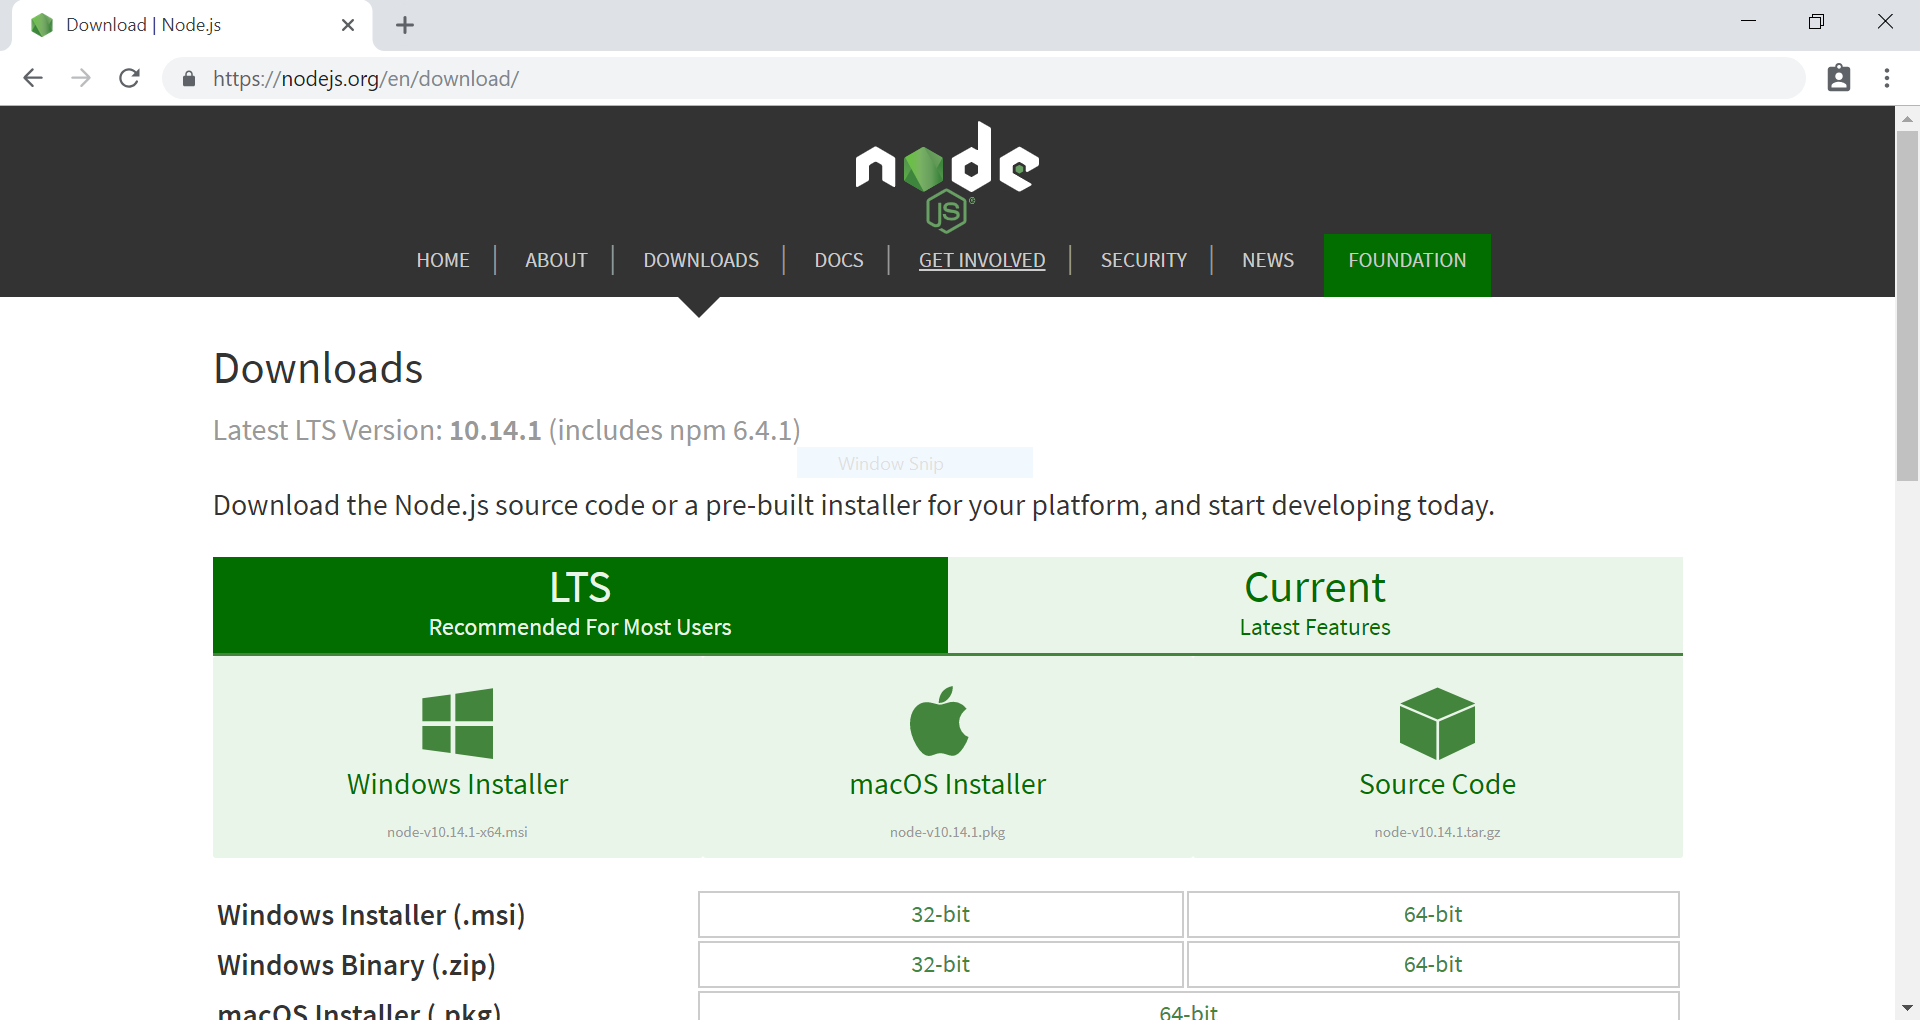
\includegraphics[width=0.6\columnwidth]{images/appendixA/Nodejs-download-page.PNG}
	      		\footcaption{Node.js official download page}
	      	\end{figure}
	      \end{center}
	      \footnotetext{Source: \url{https://nodejs.org/en/download/}} 
	\item Follow the instruction of setup wizard and install Node.js
	      \begin{center}
	      	\begin{figure}[H]
	      		\centering
	      		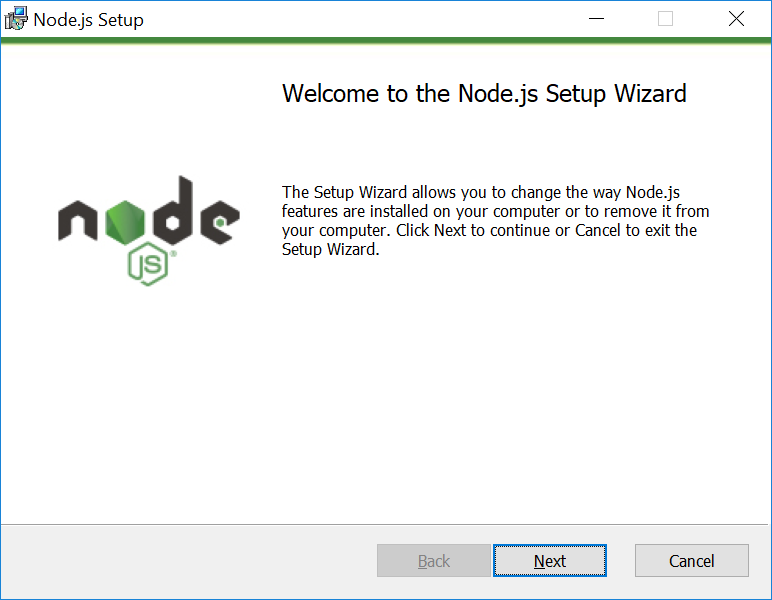
\includegraphics[width=0.6\columnwidth]{images/appendixA/Nodejs-setup.PNG}
	      		\footcaption{Node.js Setup Wizard}
	      	\end{figure}
	      \end{center}
	      \footnotetext{Source: Node.js Setup Wizard} 
	\item To verify installation, open \textit{Window Command Prompt} and enter following command: \verb+node -v+
	      \begin{center}
	      	\begin{figure}[H]
	      		\centering
	      		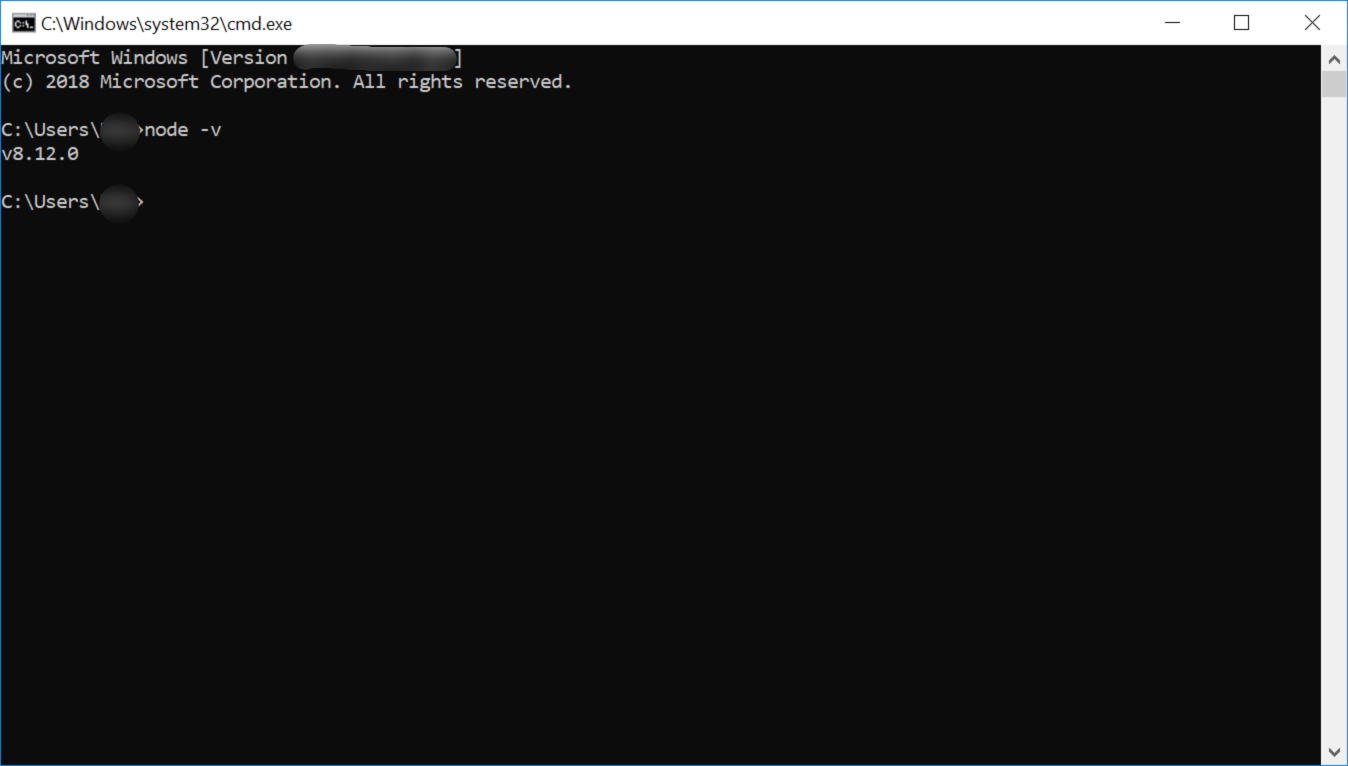
\includegraphics[width=0.6\columnwidth]{images/appendixA/Nodejs-verify-install.PNG}
	      		\footcaption{Node.js installation verification}
	      	\end{figure}
	      \end{center}
	      \footnotetext{Source: Window Command Prompt} 
\end{enumerate}
\tocless\subsection{Google Cloud Platform}
\begin{enumerate}
	\item Create an account and a new project on \textit{Google Cloud Platform} from \href{https://cloud.google.com/}{https://cloud.google.com/}
	      \begin{center}
	      	\begin{figure}[H]
	      		\centering
	      		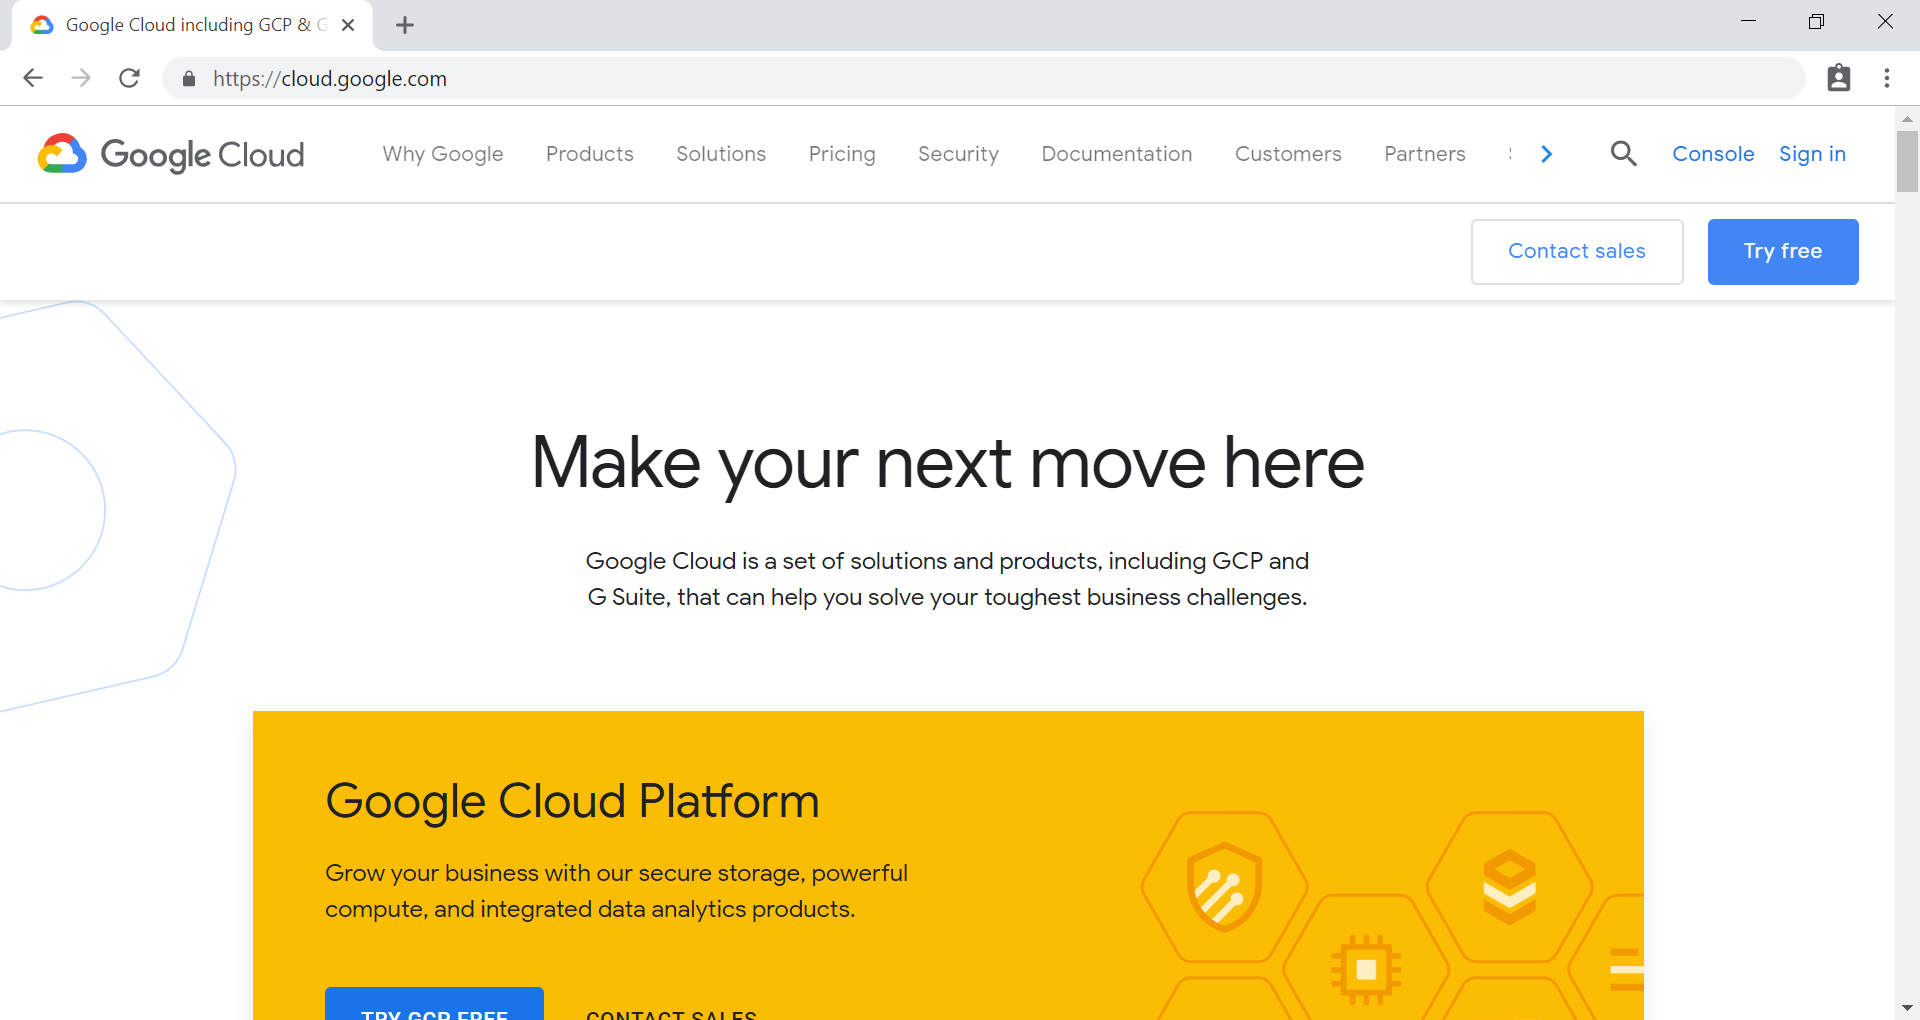
\includegraphics[width=0.6\columnwidth]{images/appendixA/GCP-homepage.PNG}
	      		\footcaption{Google Cloud Platform homepage}
	      	\end{figure}
	      \end{center}
	      \begin{center}
	      	\begin{figure}[H]
	      		\centering
	      		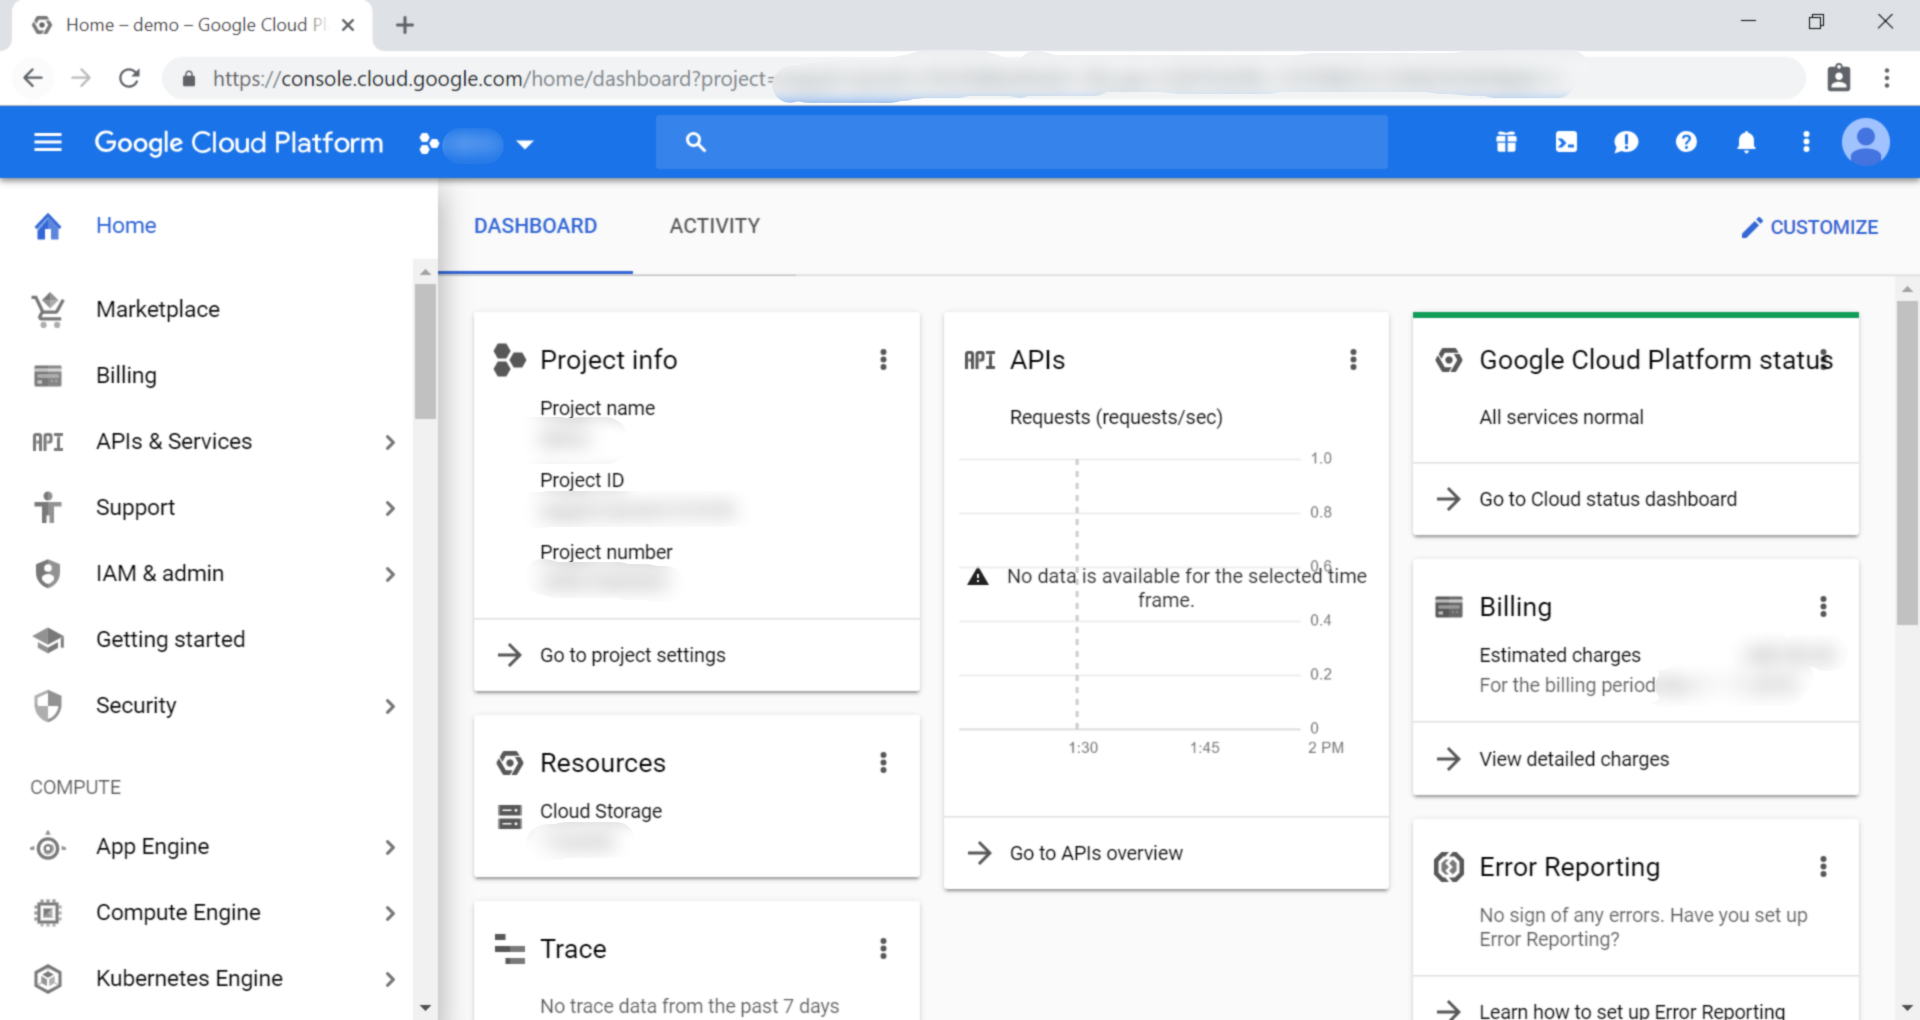
\includegraphics[width=0.6\columnwidth]{images/appendixA/GCP-console.PNG}
	      		\footcaption{Google Cloud Platform console}
	      	\end{figure}
	      \end{center}
	      \footnotetext{Source: \url{https://cloud.google.com/}} 
	\item Create \textit{Google Cloud Storage Bucket}. From the console, open navigation menu, and select \textit{Storage}
	      \begin{center}
	      	\begin{figure}[H]
	      		\centering
	      		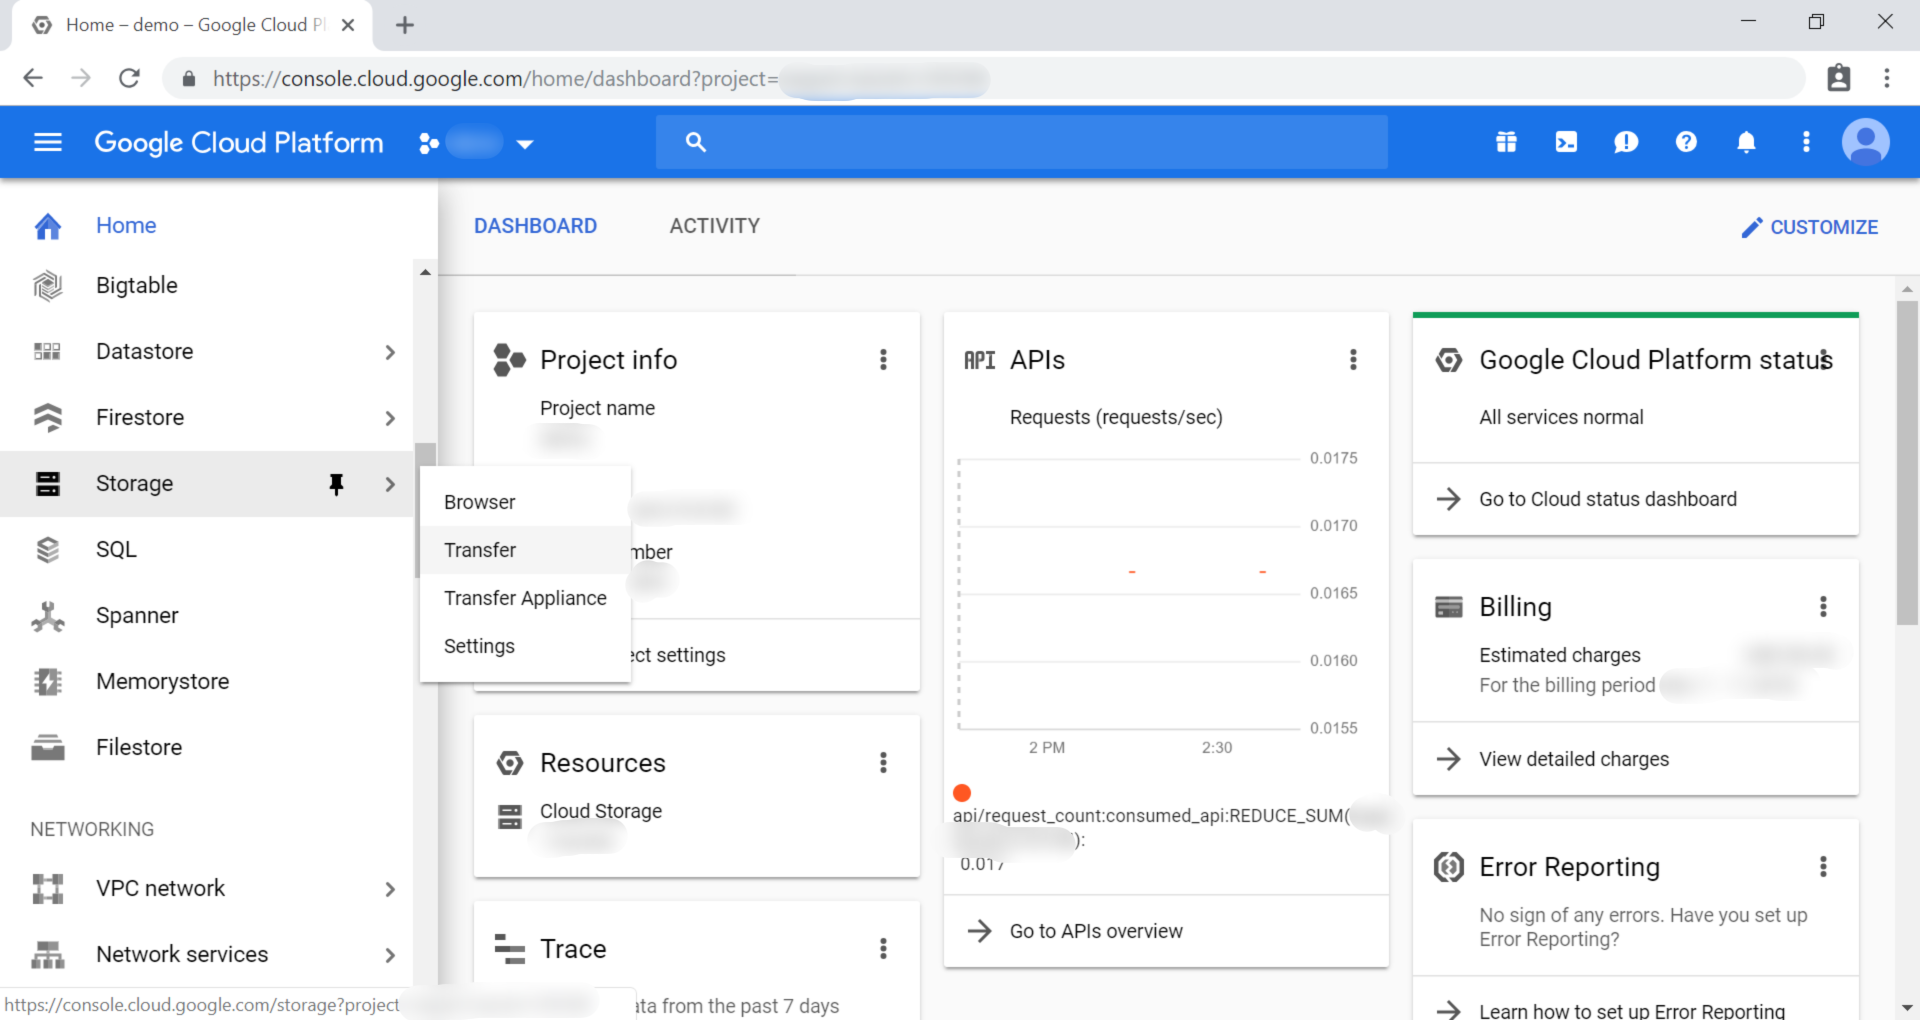
\includegraphics[width=0.6\columnwidth]{images/appendixA/GCP-navigate-Storage.PNG}
	      		\footcaption{Google Cloud Platform: Navigation Menu > Storage}
	      	\end{figure}
	      \end{center}
	      \footnotetext{Source: \url{https://cloud.google.com/}} 
	\item Click \textit{Create bucket} button and provide required information
	      \begin{center}
	      	\begin{figure}[H]
	      		\centering
	      		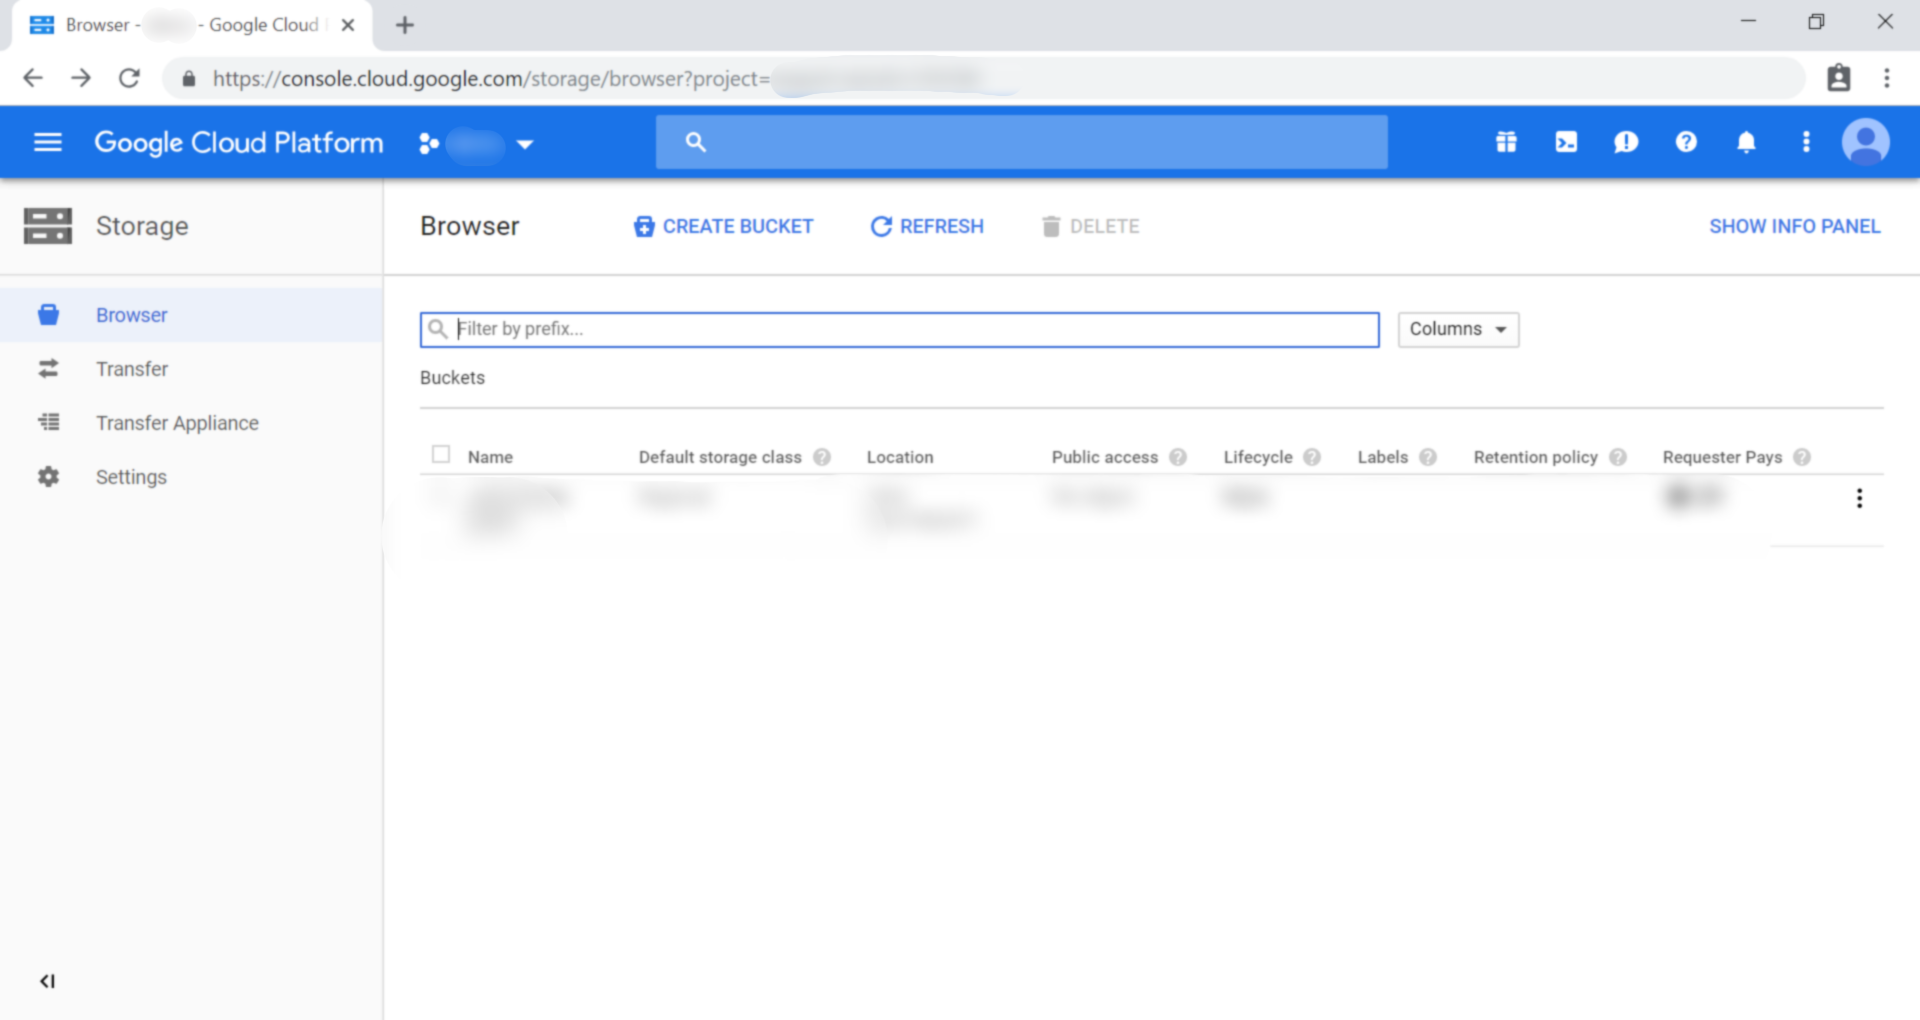
\includegraphics[width=0.6\columnwidth]{images/appendixA/GCP-Storage.PNG}
	      		\footcaption{Google Cloud Storage Management}
	      	\end{figure}
	      	\begin{figure}[H]
	      		\centering
	      		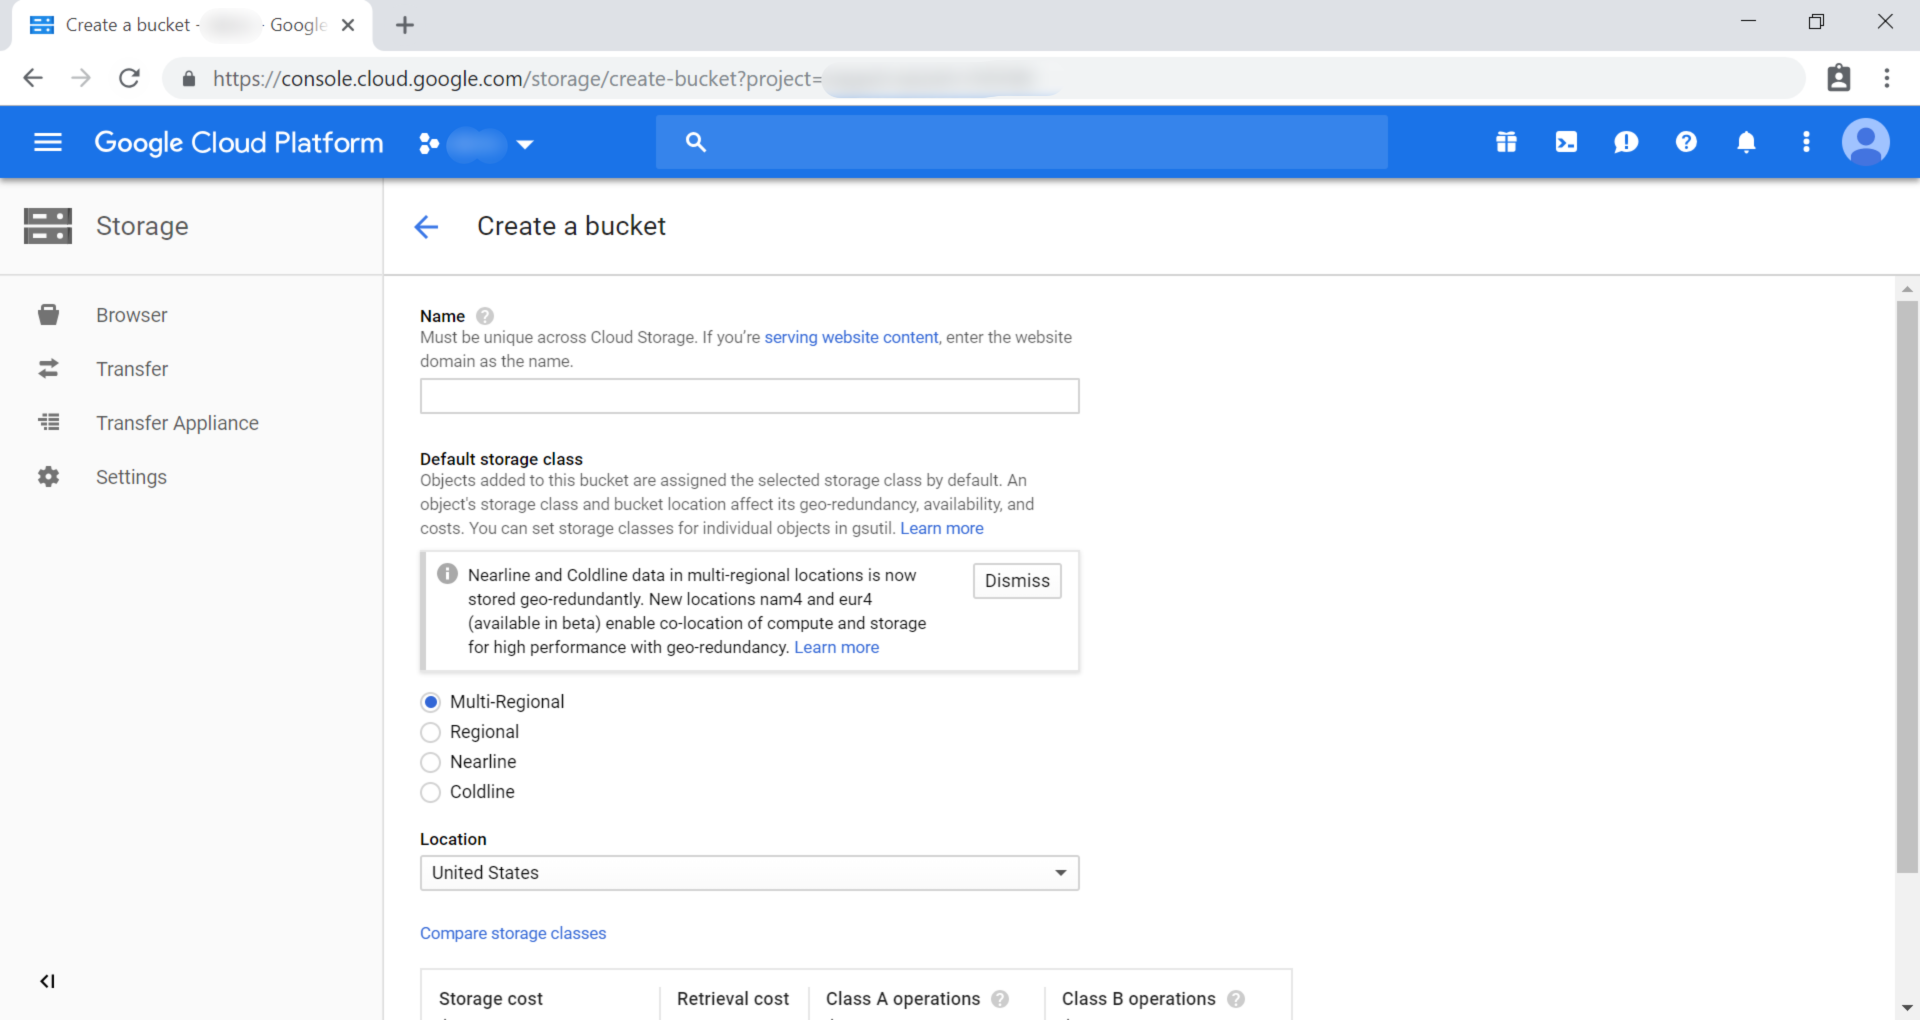
\includegraphics[width=0.6\columnwidth]{images/appendixA/GCP-Storage-create-bucket.PNG}
	      		\footcaption{Google Cloud Storage: Create Bucket}
	      	\end{figure}
	      \end{center}
	      \footnotetext{Source: \url{https://cloud.google.com/}}
	\item Following instruction in \href{https://cloud.google.com/iam/docs/creating-managing-service-accounts#creating_a_service_account}{https://cloud.google.com/iam/docs/creating-managing-service-accounts\#creating\_a\_service\_account} to create a \textit{Service Account} 
	\item Following instruction in \href{https://cloud.google.com/iam/docs/granting-roles-to-service-accounts#granting_access_to_a_service_account_for_a_resource}{https://cloud.google.com/iam/docs/granting-roles-to-service-accounts\#granting\_access\_to\_a\_service\_account\_for\_a\_resource} to grant role \textit{Storage Admin} for created \textit{Service Account}
	\item Following instruction in \href{https://cloud.google.com/iam/docs/creating-managing-service-account-keys#creating_service_account_keys}{https://cloud.google.com/iam/docs/creating-managing-service-account-keys\#creating\_service\_account\_keys} to create a \textit{Service Account key}. Download and keep it locally.
\end{enumerate}

\tocless\subsection{mLab}
\begin{enumerate}
	\item Access \href{https://mlab.com/signup/}{https://mlab.com/signup/} and sign up an account
	      \begin{center}
	      	\begin{figure}[H]
	      		\centering
	      		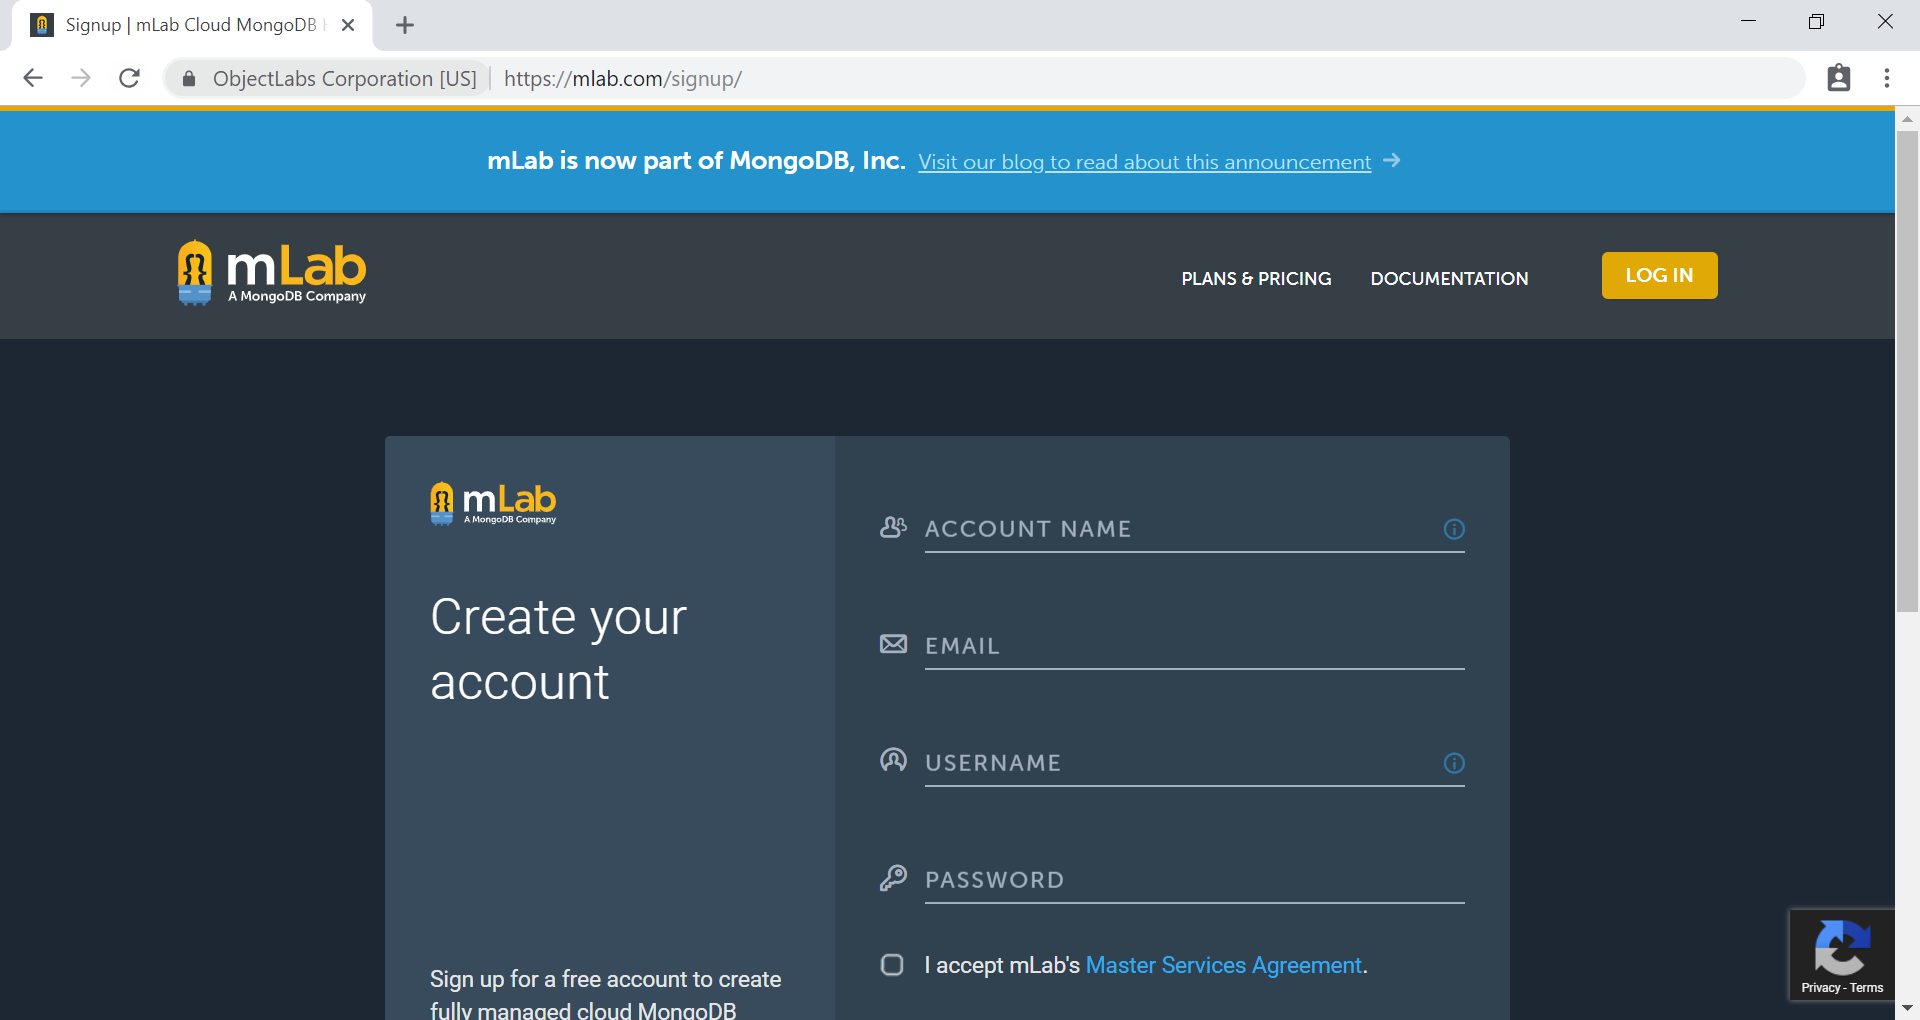
\includegraphics[width=0.6\columnwidth]{images/appendixA/mLab-sign-up.PNG}
	      		\footcaption{mLab Sign up page}
	      	\end{figure}
	      \end{center}
	      \footnotetext{Source: \url{https://mlab.com/}} 
	\item Click \textit{Create new} to create a new deployment
	      \begin{center}
	      	\begin{figure}[H]
	      		\centering
	      		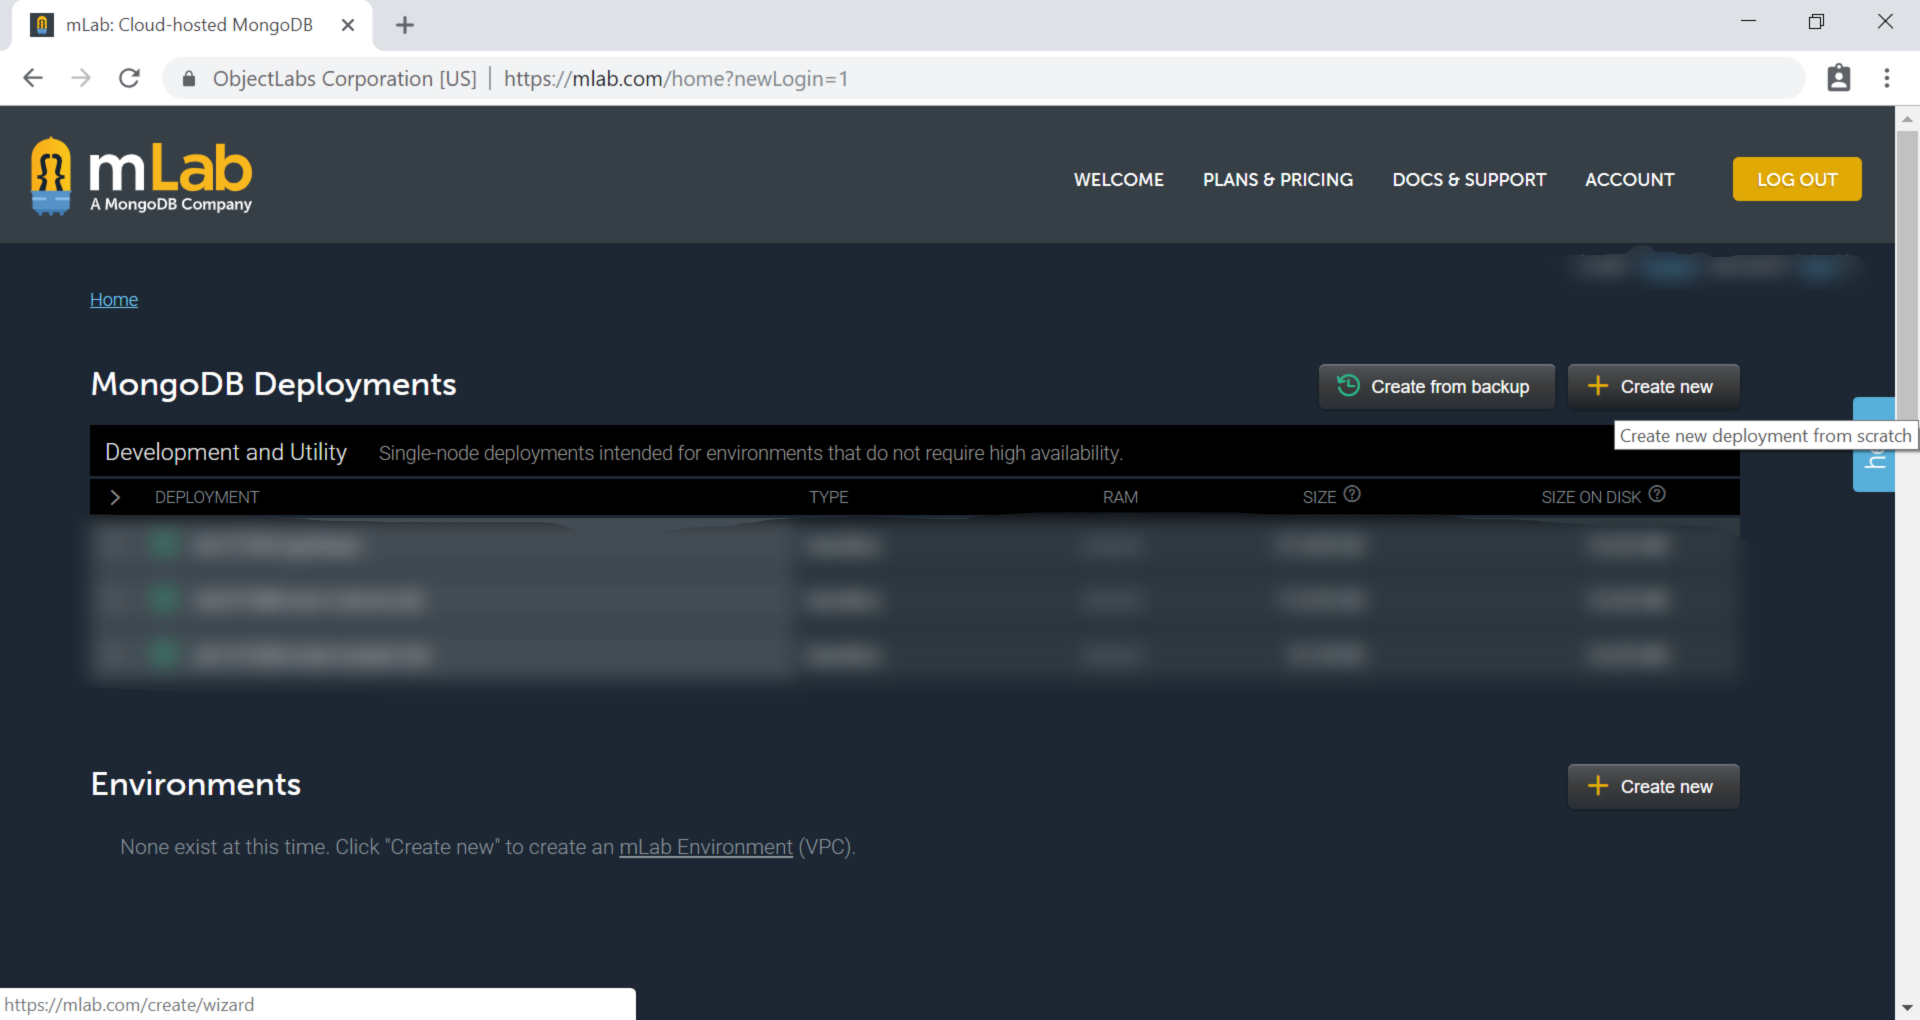
\includegraphics[width=0.6\columnwidth]{images/appendixA/mLab-create-deployment.png}
	      		\caption{mLab Control Panel}
	      	\end{figure}
	      \end{center}
	      \begin{center}
	      	\begin{figure}[H]
	      		\centering
	      		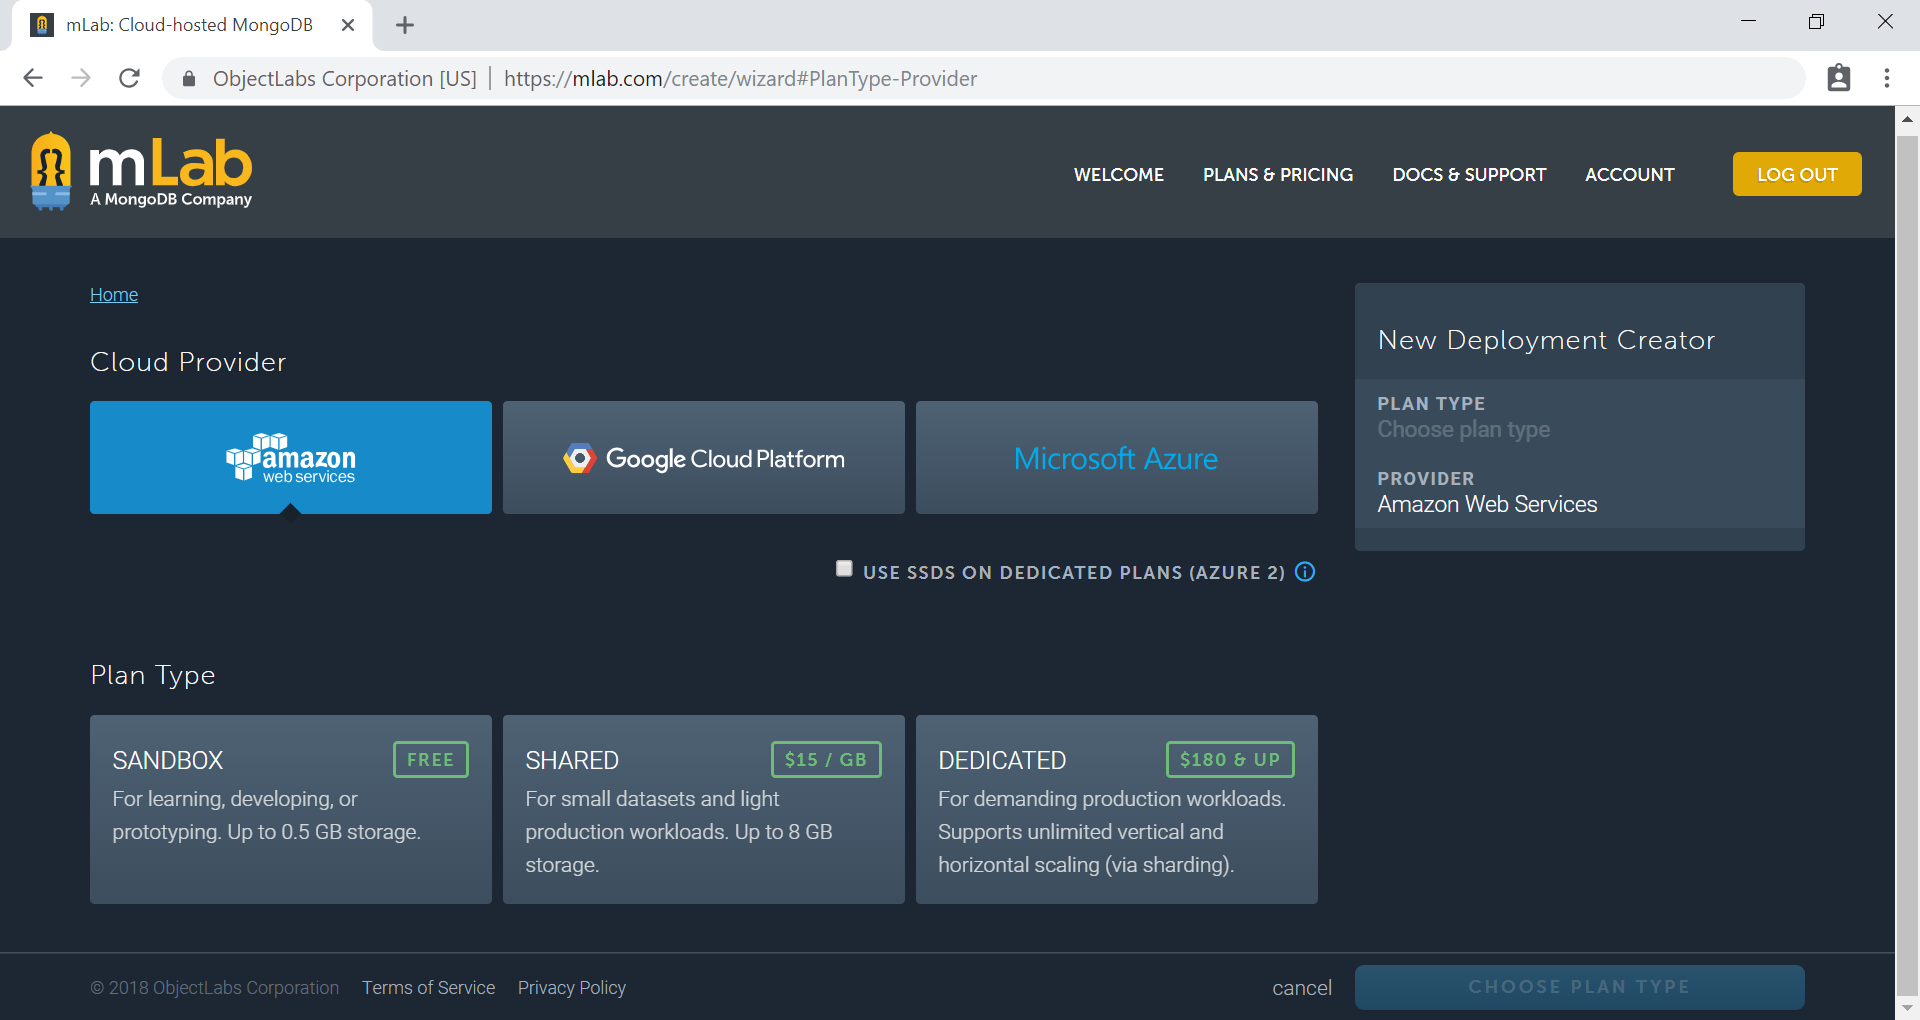
\includegraphics[width=0.6\columnwidth]{images/appendixA/mLab-create-deployment-2.PNG}
	      		\caption{mLab Create new deployment page}
	      	\end{figure}
	      \end{center}
	\item Click \textit{Users} and select \textit{Add database user}
	      \begin{center}
	      	\begin{figure}[H]
	      		\centering
	      		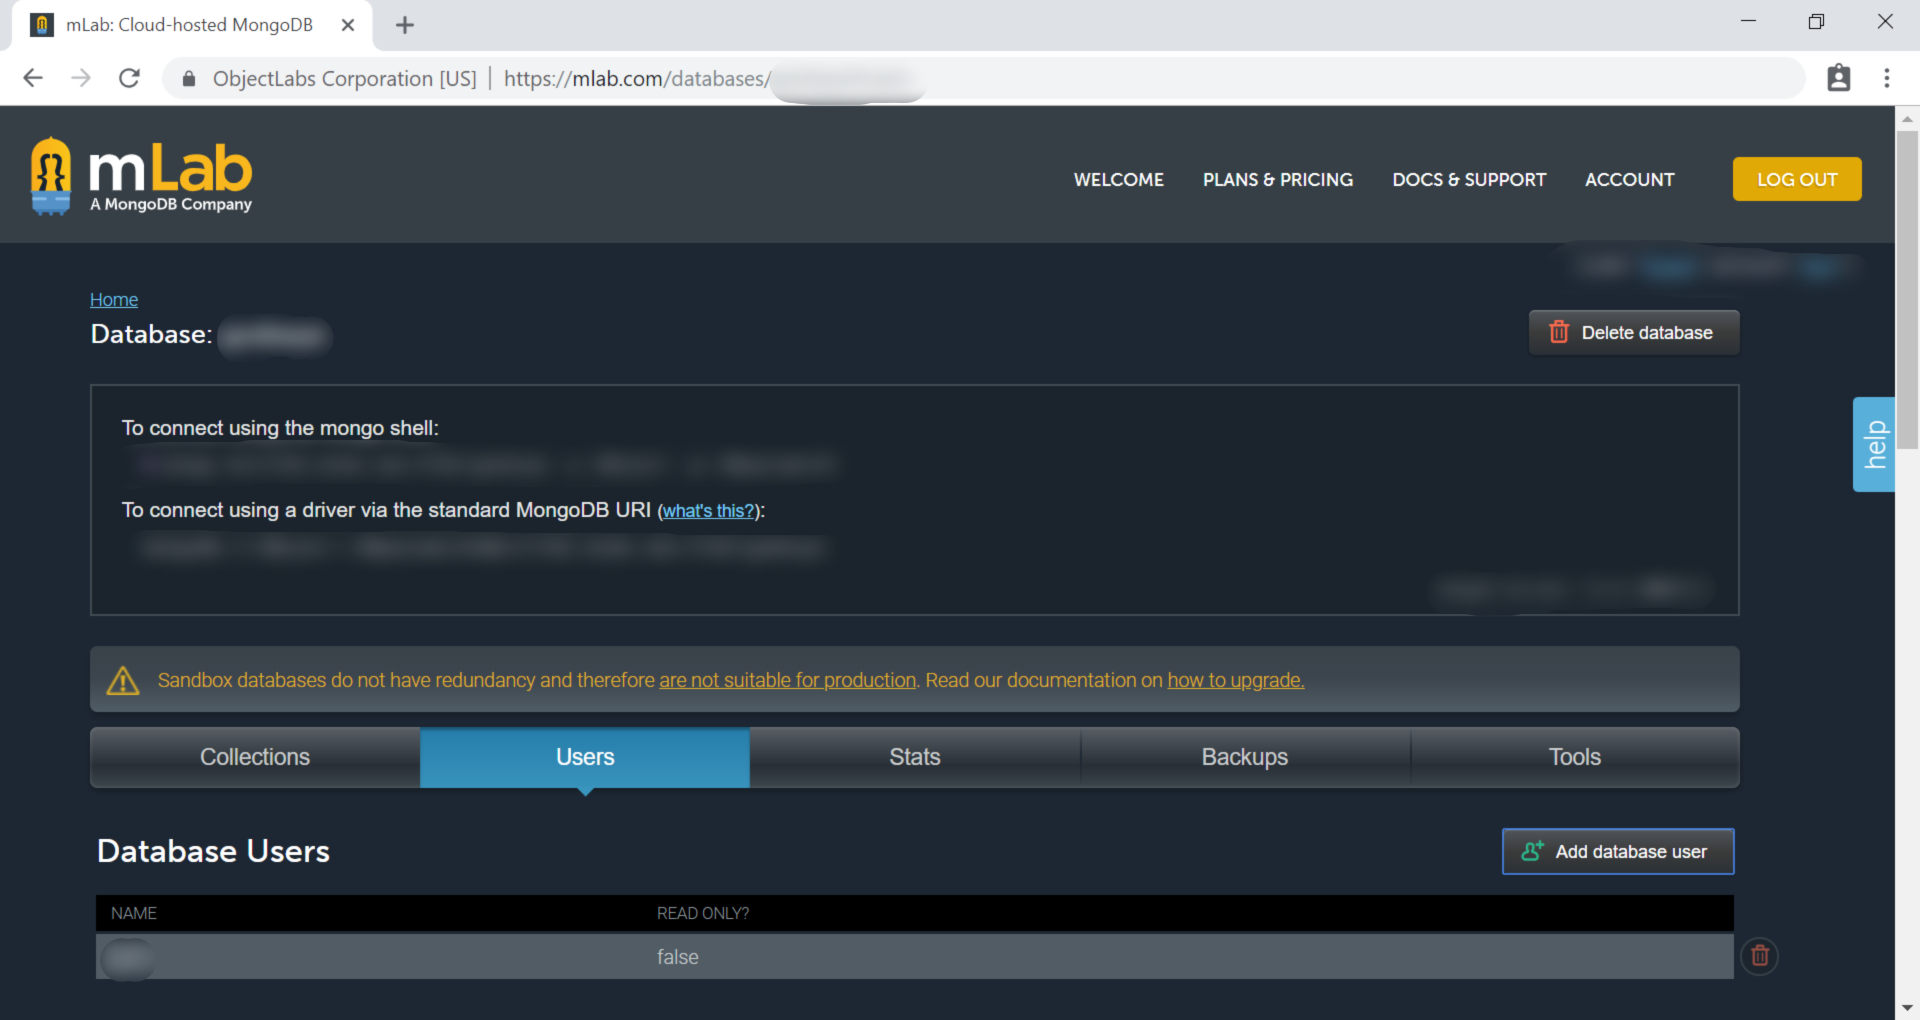
\includegraphics[width=0.6\columnwidth]{images/appendixA/mLab-create-user.png}
	      		\caption{mLab Users tab}
	      	\end{figure}
	      \end{center}
	      \begin{center}
	      	\begin{figure}[H]
	      		\centering
	      		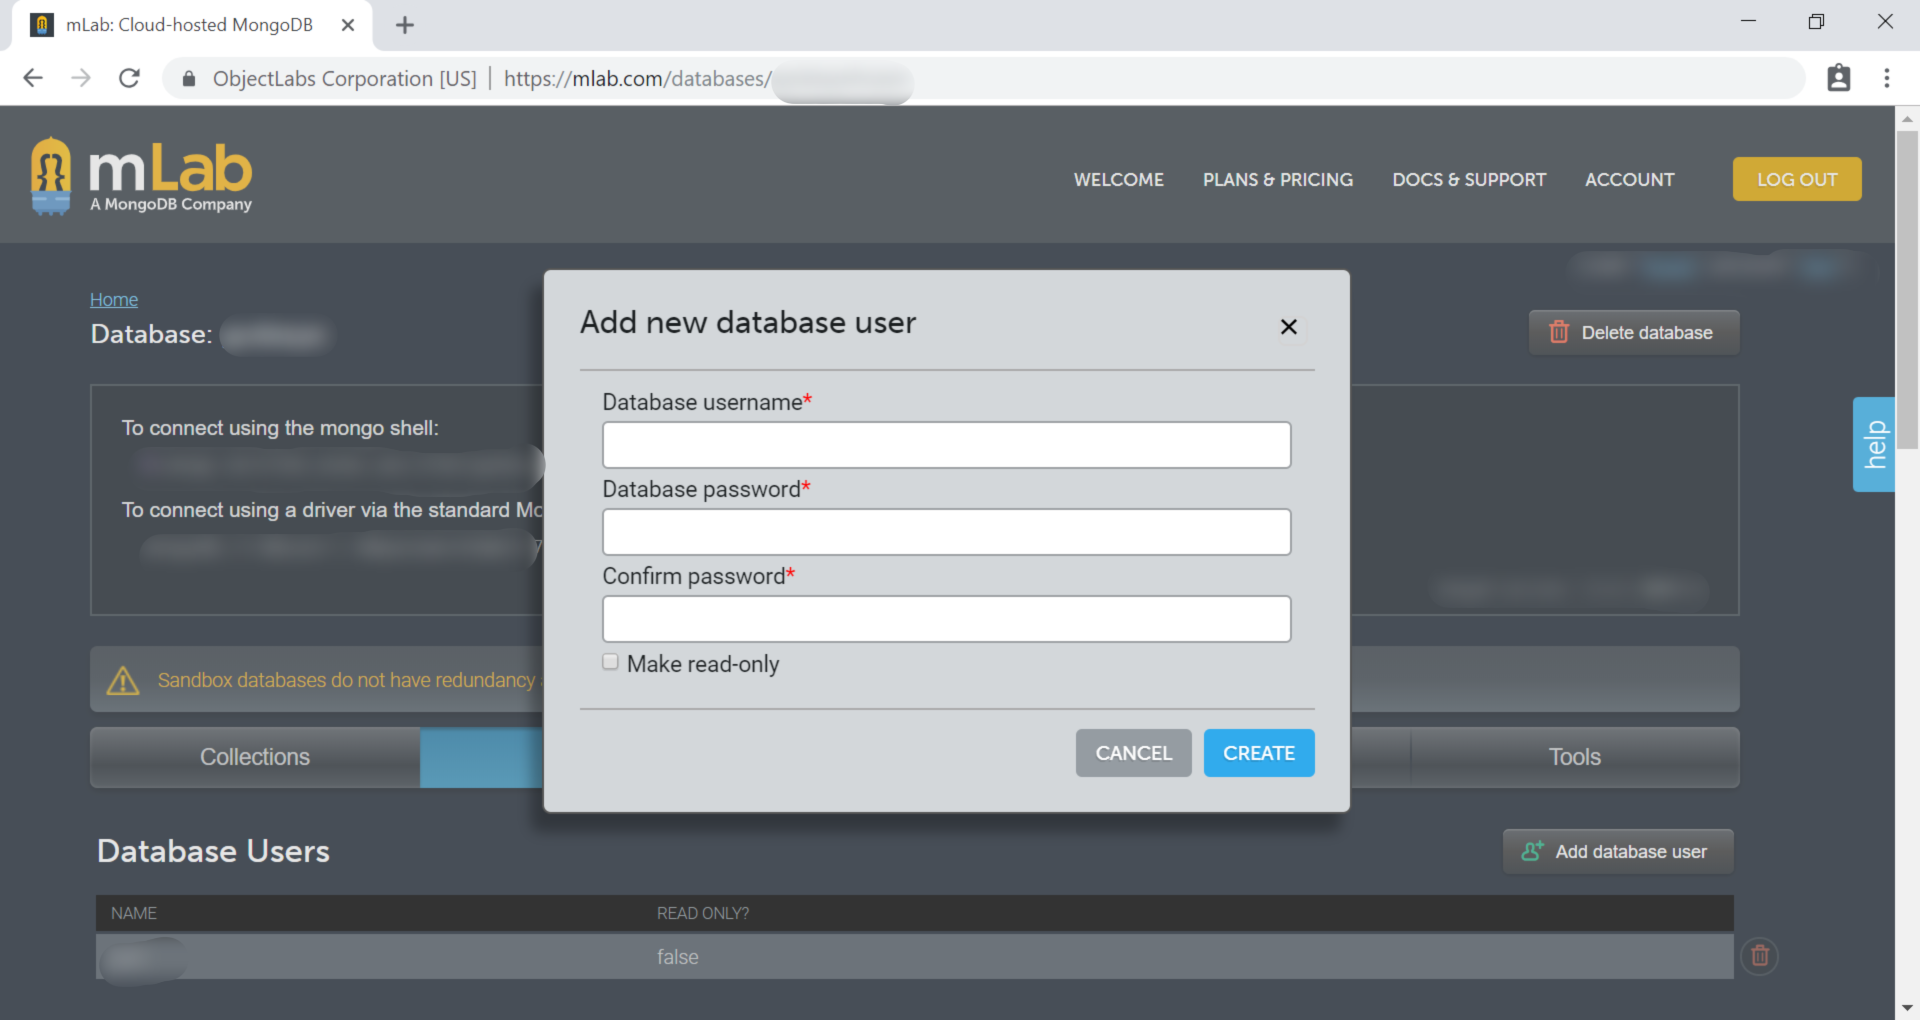
\includegraphics[width=0.6\columnwidth]{images/appendixA/mLab-create-user-2.png}
	      		\caption{mLab Add new database user pop-up}
	      	\end{figure}
	      \end{center}
\end{enumerate}

\tocless\subsection{Microsoft Cognitive Services}
\begin{enumerate}
	\item Access \href{https://azure.microsoft.com/en-us/free}{https://azure.microsoft.com/en-us/free} and create an Azure account. For more detail, please follow this instruction \href{https://docs.microsoft.com/en-us/azure/cognitive-services/cognitive-services-apis-create-account}{https://docs.microsoft.com/en-us/azure/cognitive-services/cognitive-services-apis-create-account}
	      \begin{center}
	      	\begin{figure}[H]
	      		\centering
	      		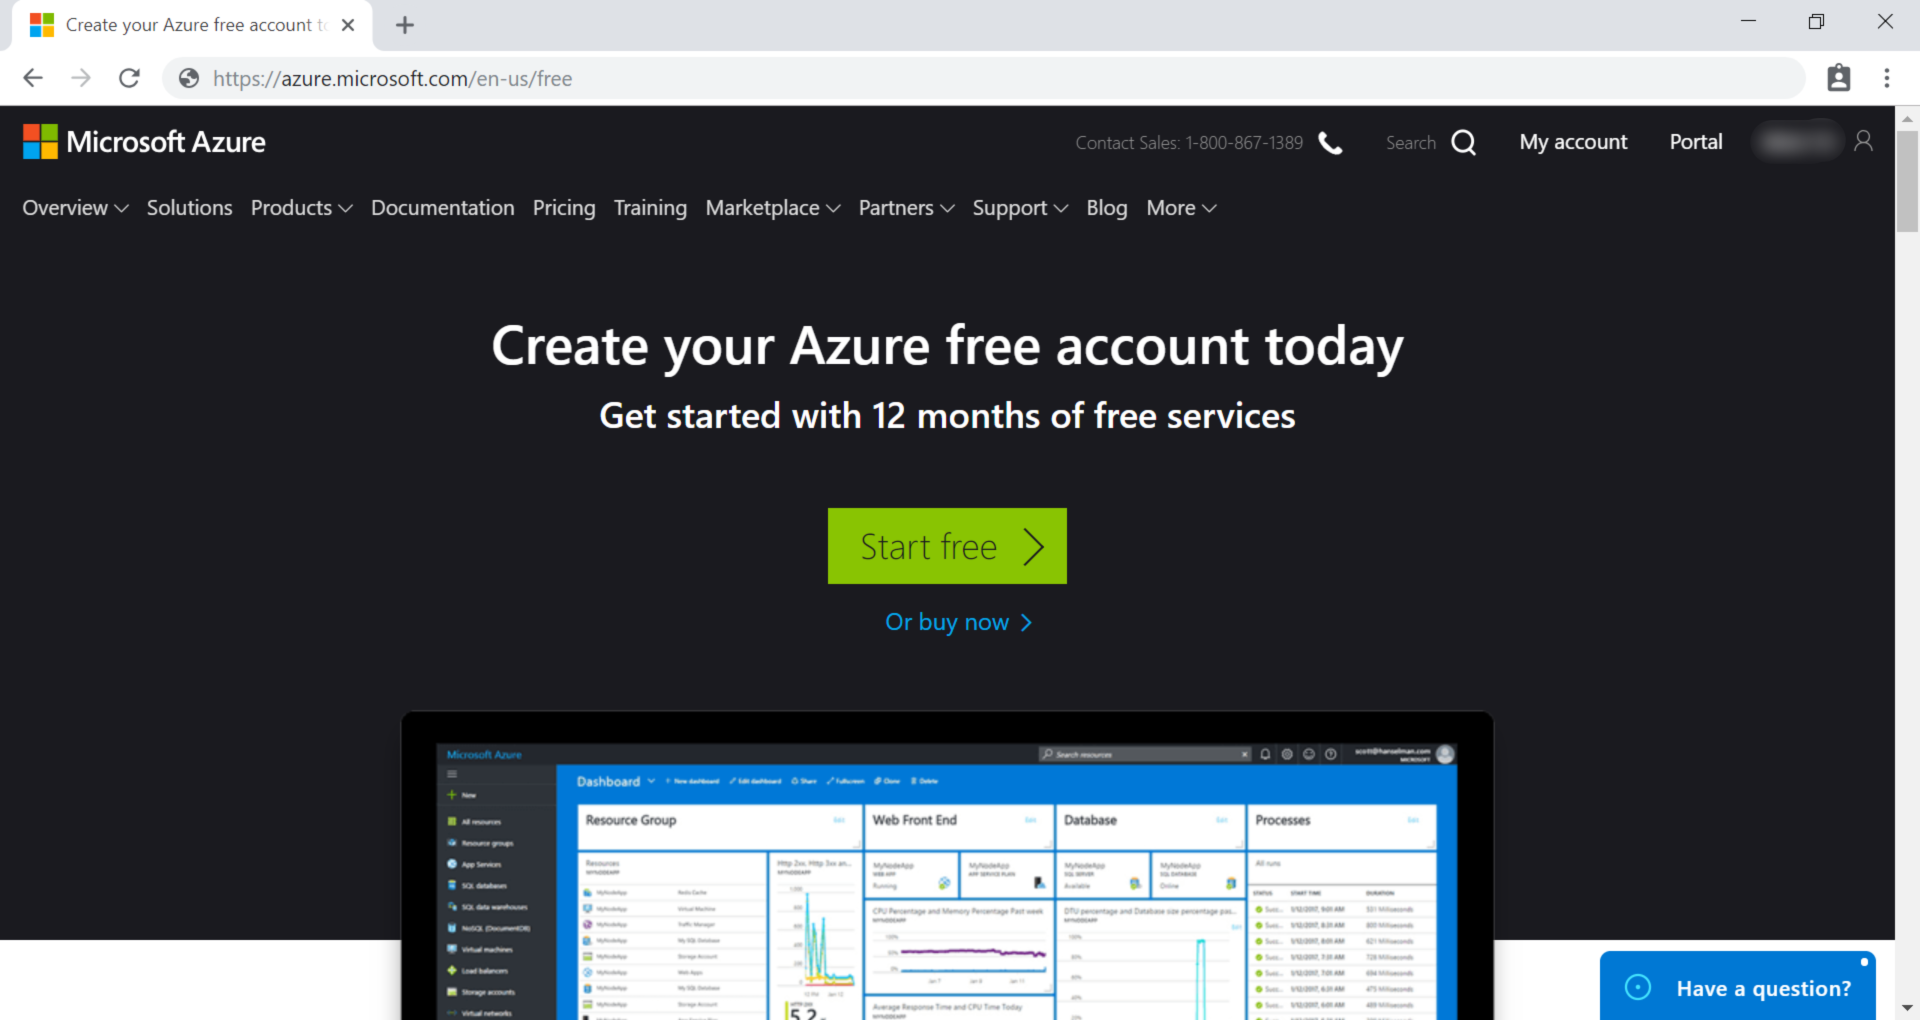
\includegraphics[width=0.6\columnwidth]{images/appendixA/Azure-homepage.png}
	      		\caption{Microsoft Azure homepage}
	      	\end{figure}
	      \end{center}
	\item Create and subscribe to  Azure Cognitive Services: Face
	      \begin{center}
	      	\begin{figure}[H]
	      		\centering
	      		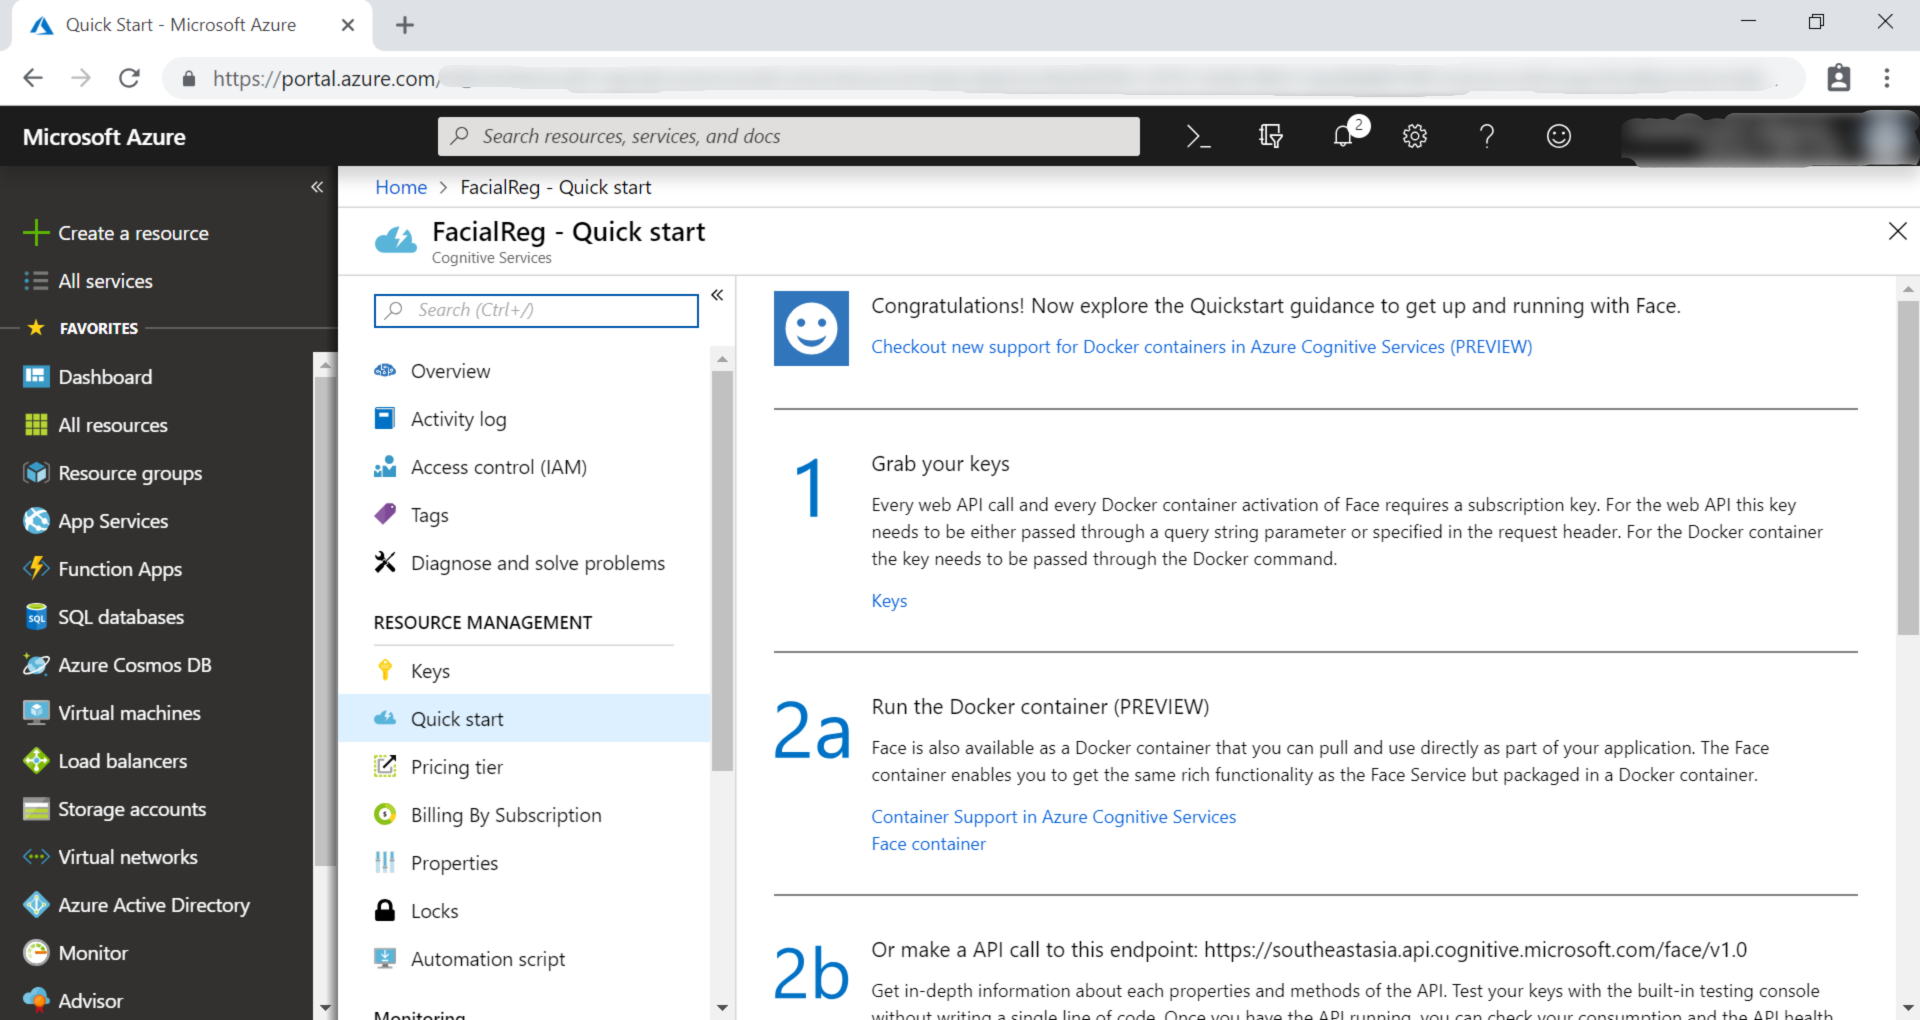
\includegraphics[width=0.6\columnwidth]{images/appendixA/Azure-subscribe-facial-reg.png}
	      		\caption{Azure Face Recognition}
	      	\end{figure}
	      \end{center}
	\item Grab API keys
\end{enumerate}

\tocless\subsection{Facebook Account Kit}
\begin{enumerate}
	\item Follow this documentation from \href{https://developers.facebook.com/docs/accountkit/webjs}{https://developers.facebook.com/docs/accountkit/webjs} to integrate Facebook Account Kit for Web. A Facebook Developer account is required.
	      \begin{center}
	      	\begin{figure}[H]
	      		\centering
	      		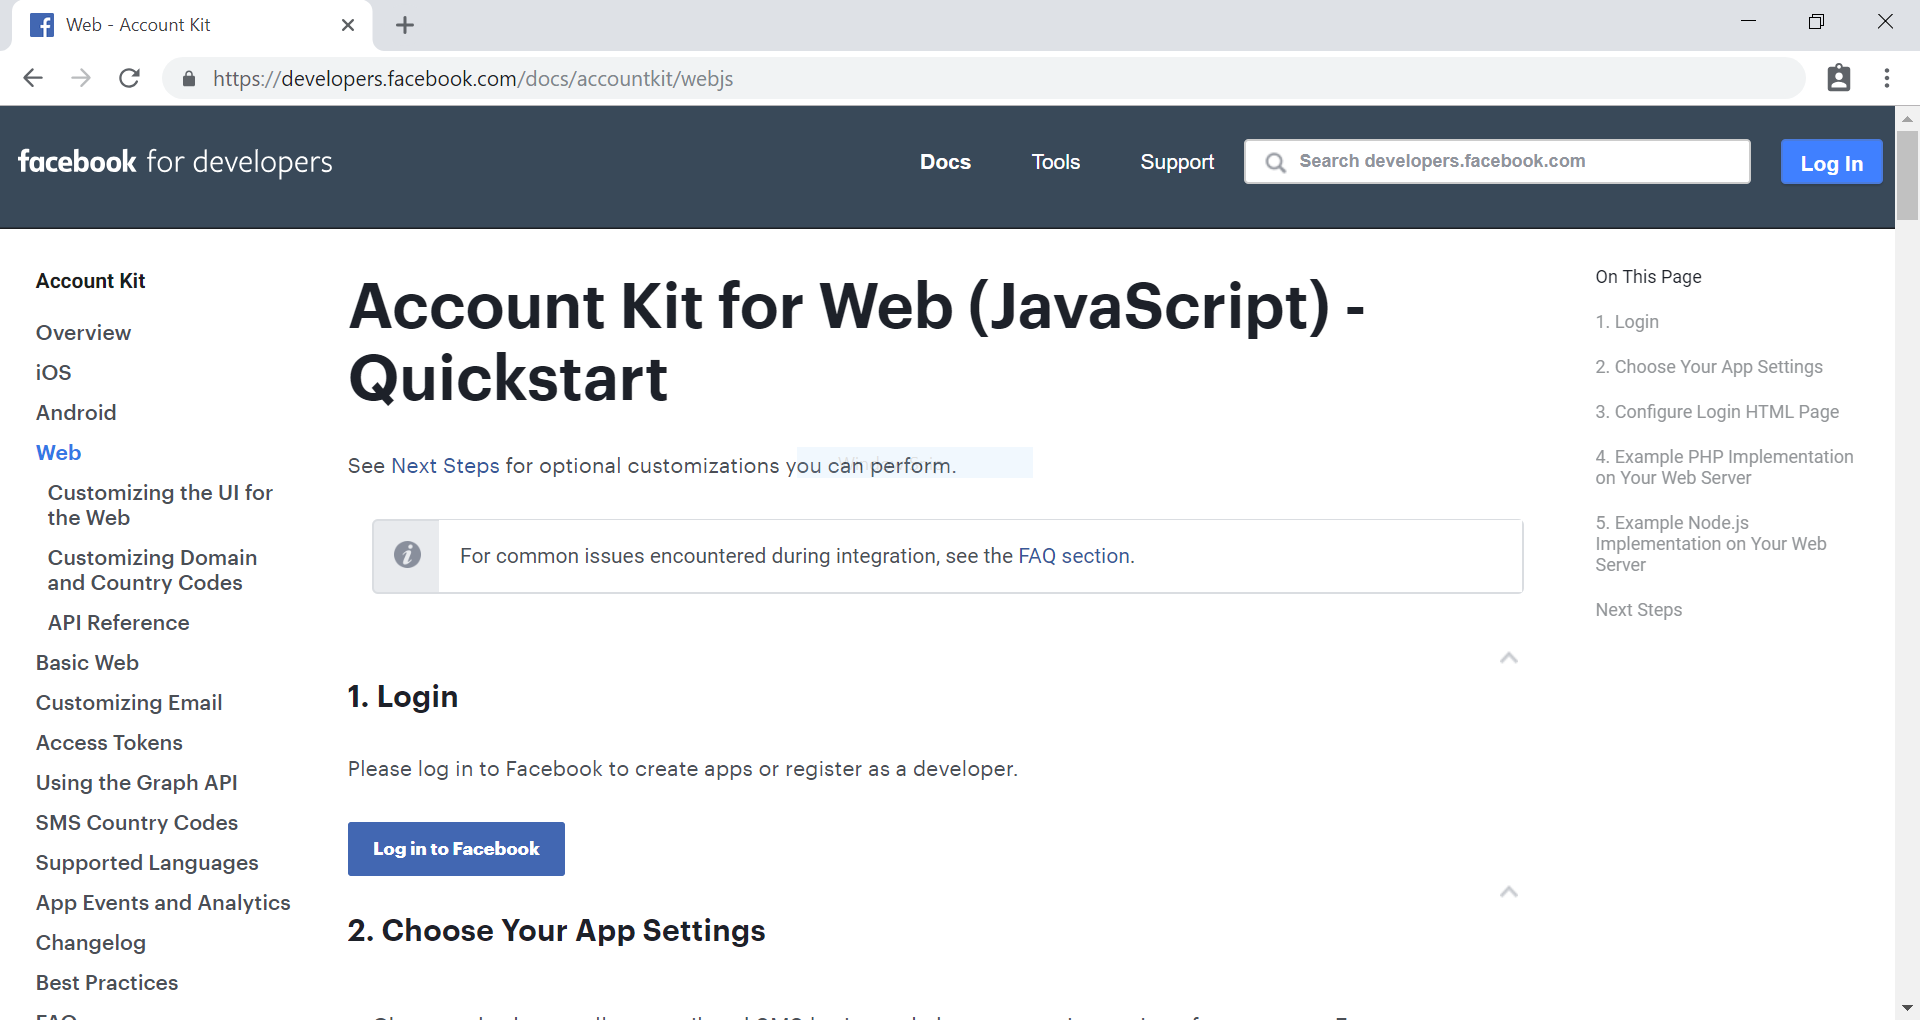
\includegraphics[width=0.6\columnwidth]{images/appendixA/Facebook-AccountKit-Docs.PNG}
	      		\caption{Facebook Account Kit for Web}
	      	\end{figure}
	      \end{center}
	\item After successfully integrated, Account Kit will appear below application name with a check mark.
	      \begin{center}
	      	\begin{figure}[H]
	      		\centering
	      		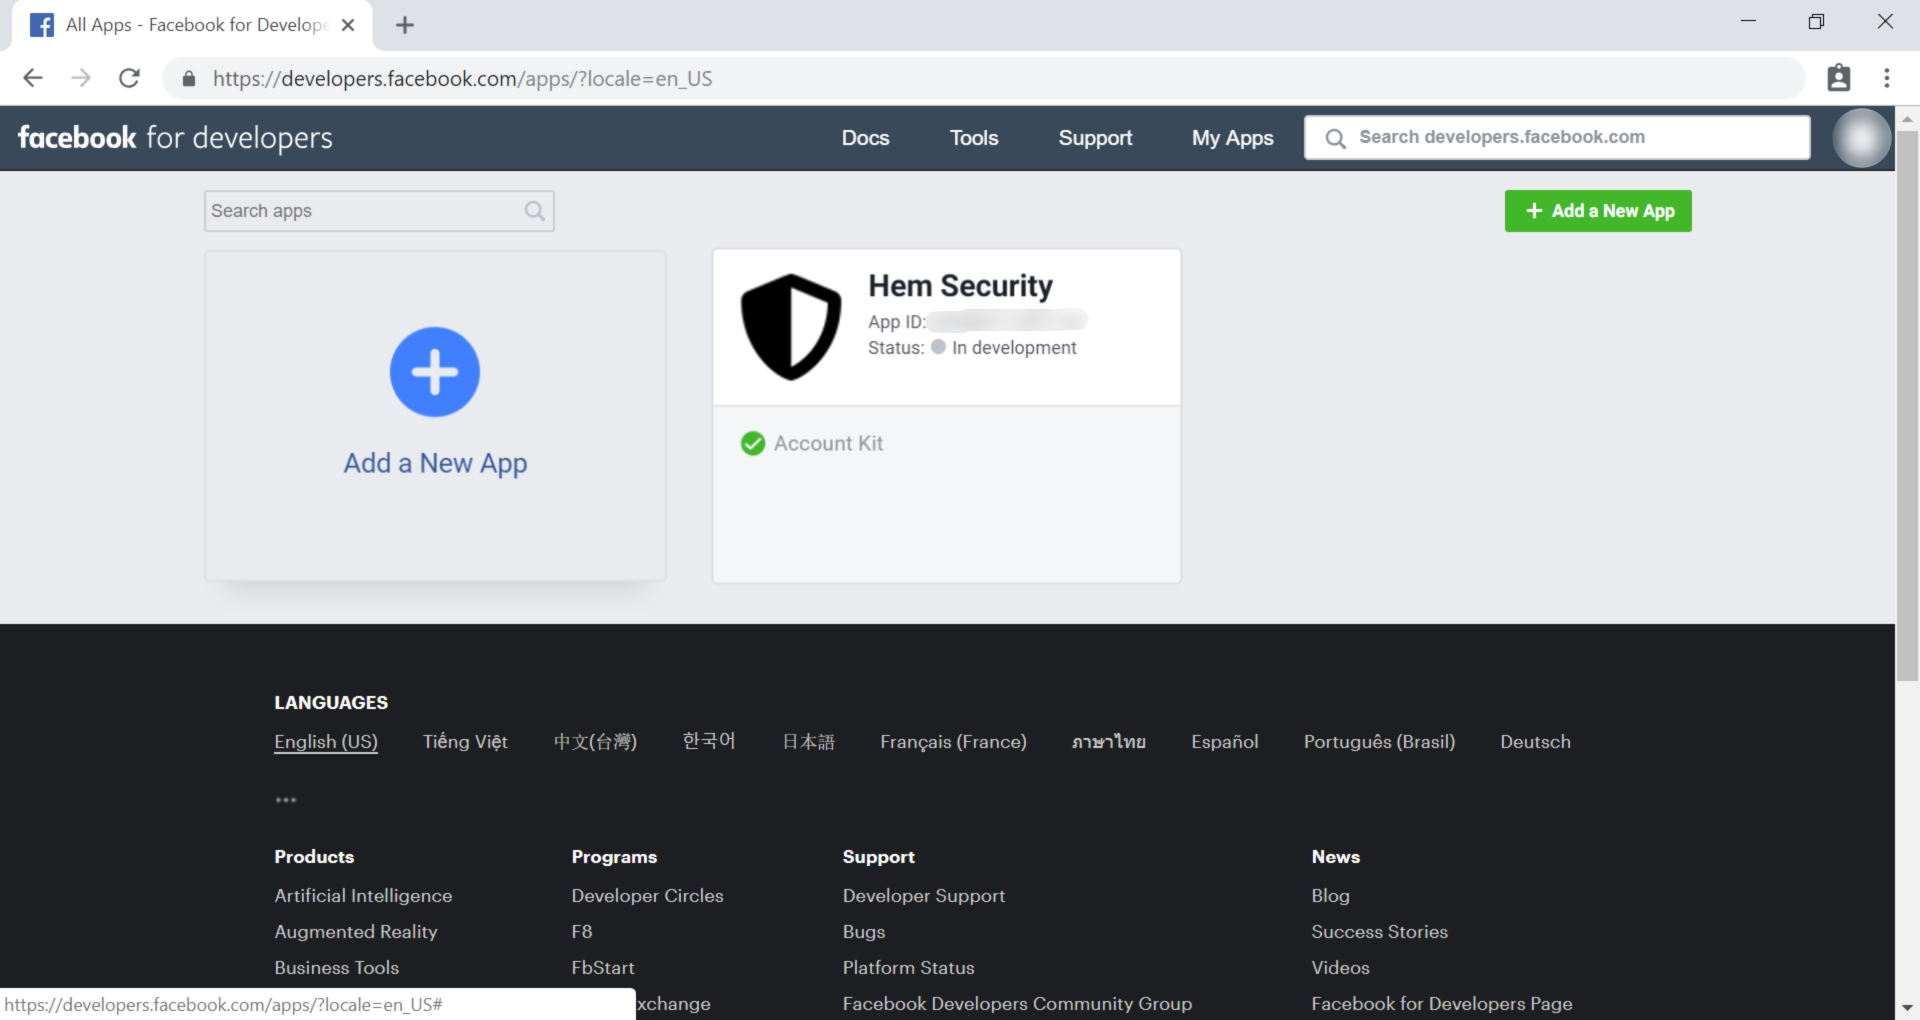
\includegraphics[width=0.6\columnwidth]{images/appendixA/Facebook-AccountKit-Integrated.png}
	      		\caption{Facebook Account Kit integrated}
	      	\end{figure}
	      \end{center}
	\item Access Account Kit Settings in application dashboard for more advanced configuration
	      \begin{center}
	      	\begin{figure}[H]
	      		\centering
	      		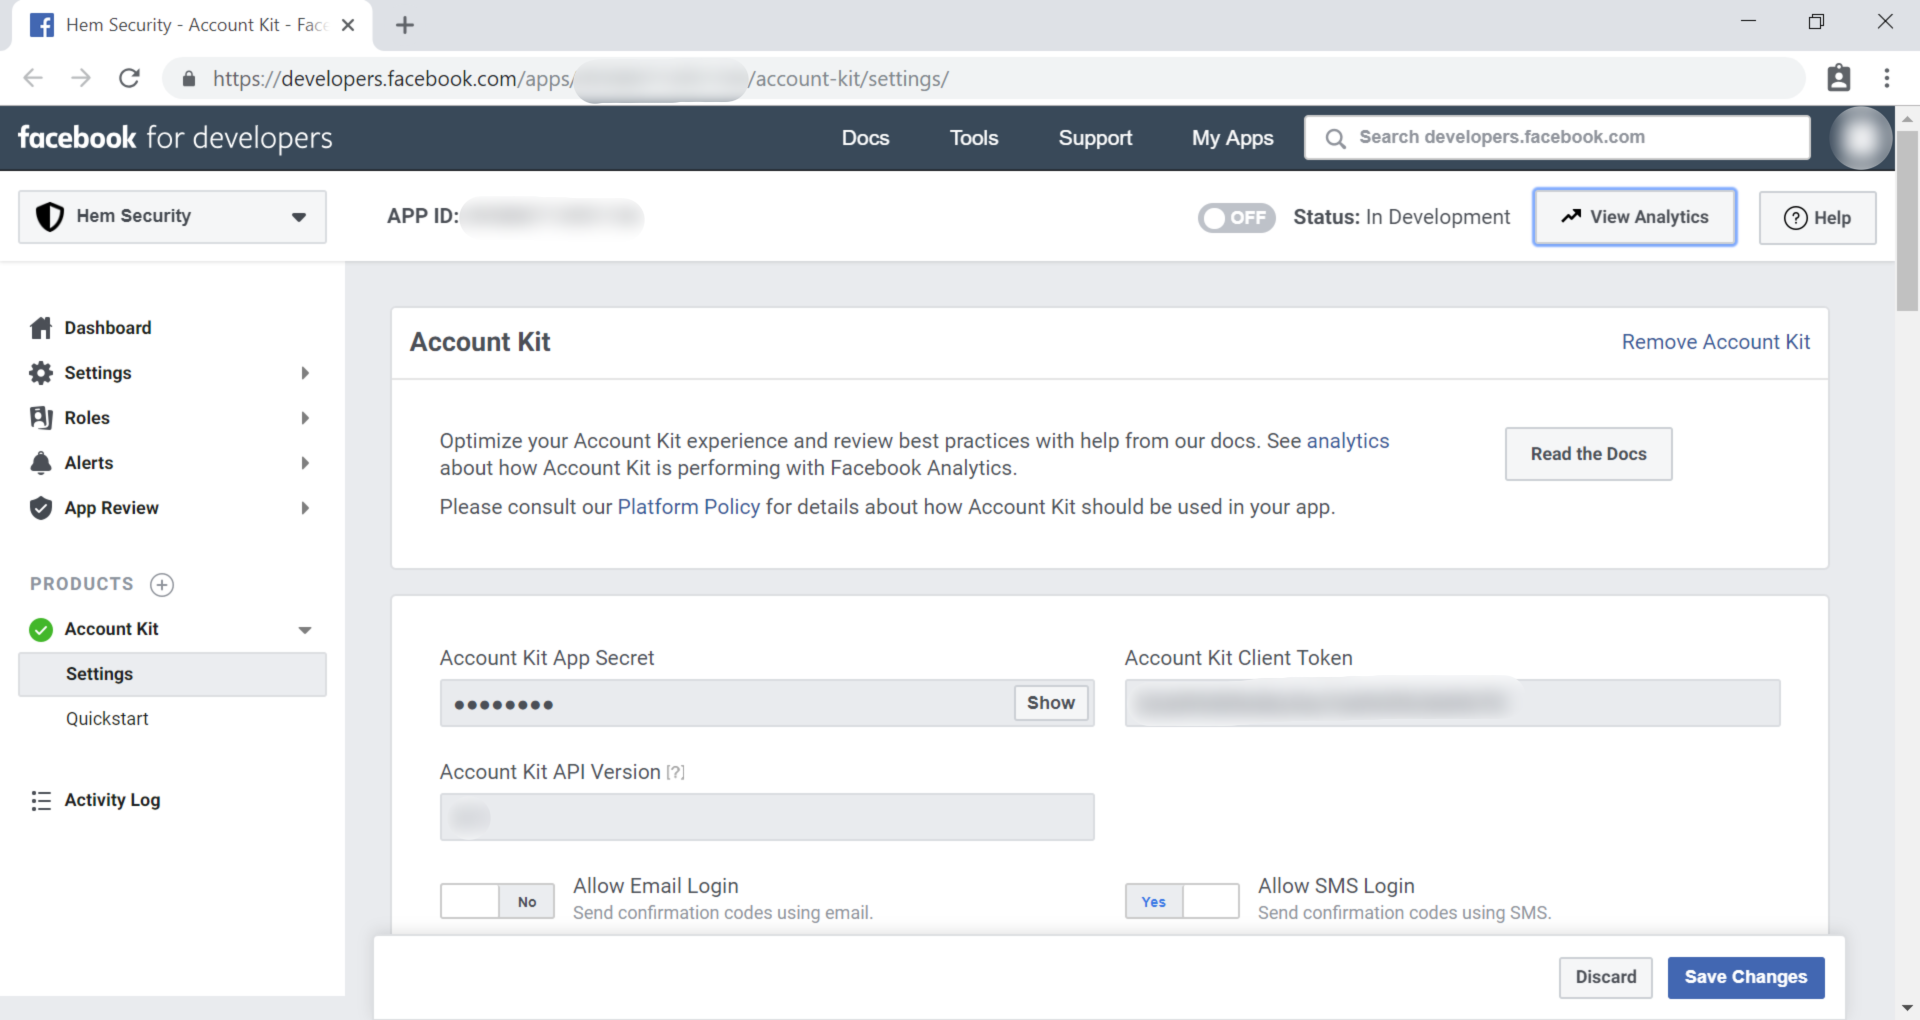
\includegraphics[width=0.6\columnwidth]{images/appendixA/Facebook-AccountKit-Settings.png}
	      		\caption{Facebook Account Kit settings}
	      	\end{figure}
	      \end{center}
\end{enumerate}

\tocless\subsection{SendGrid}
\begin{enumerate}
	\item Access SendGrid’s homepage at \href{https://sendgrid.com/}{https://sendgrid.com/} and sign up an account
	      \begin{center}
	      	\begin{figure}[H]
	      		\centering
	      		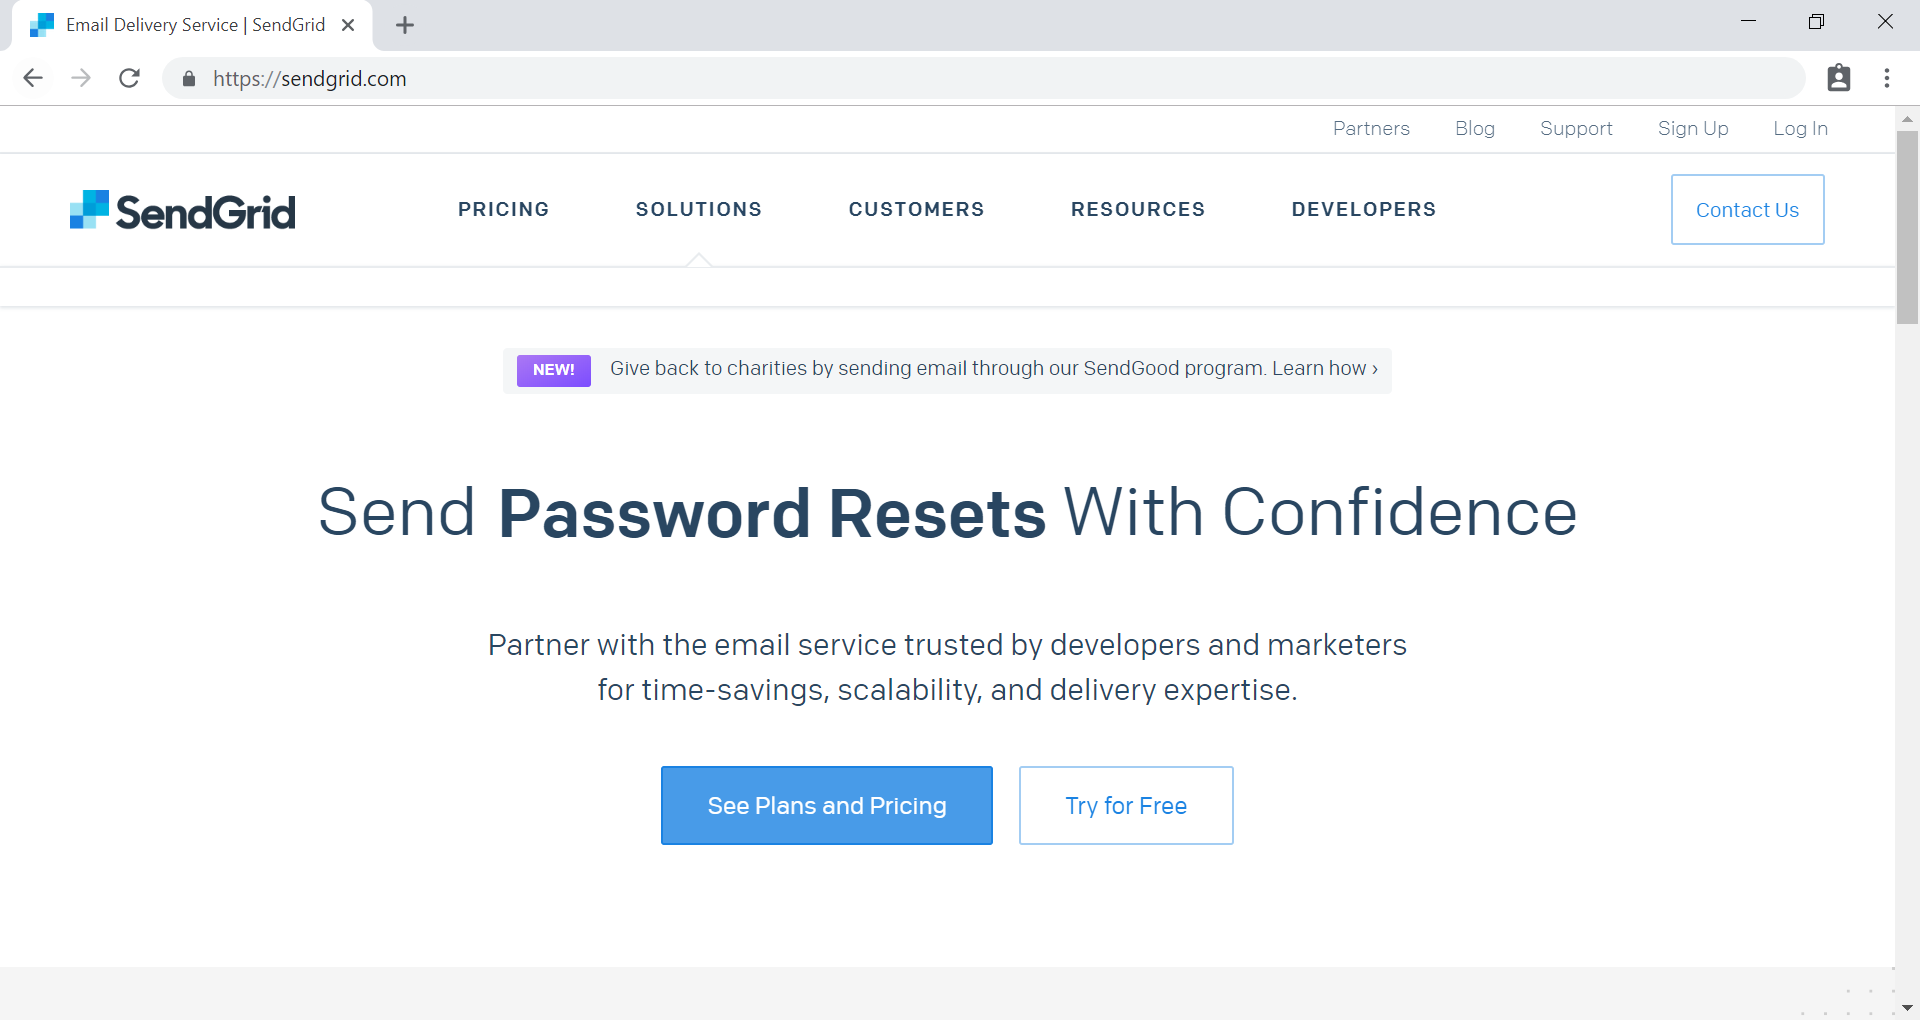
\includegraphics[width=0.6\columnwidth]{images/appendixA/SendGrid-Homepage.PNG}
	      		\caption{SendGrid homepage}
	      	\end{figure}
	      \end{center}
	      \begin{center}
	      	\begin{figure}[H]
	      		\centering
	      		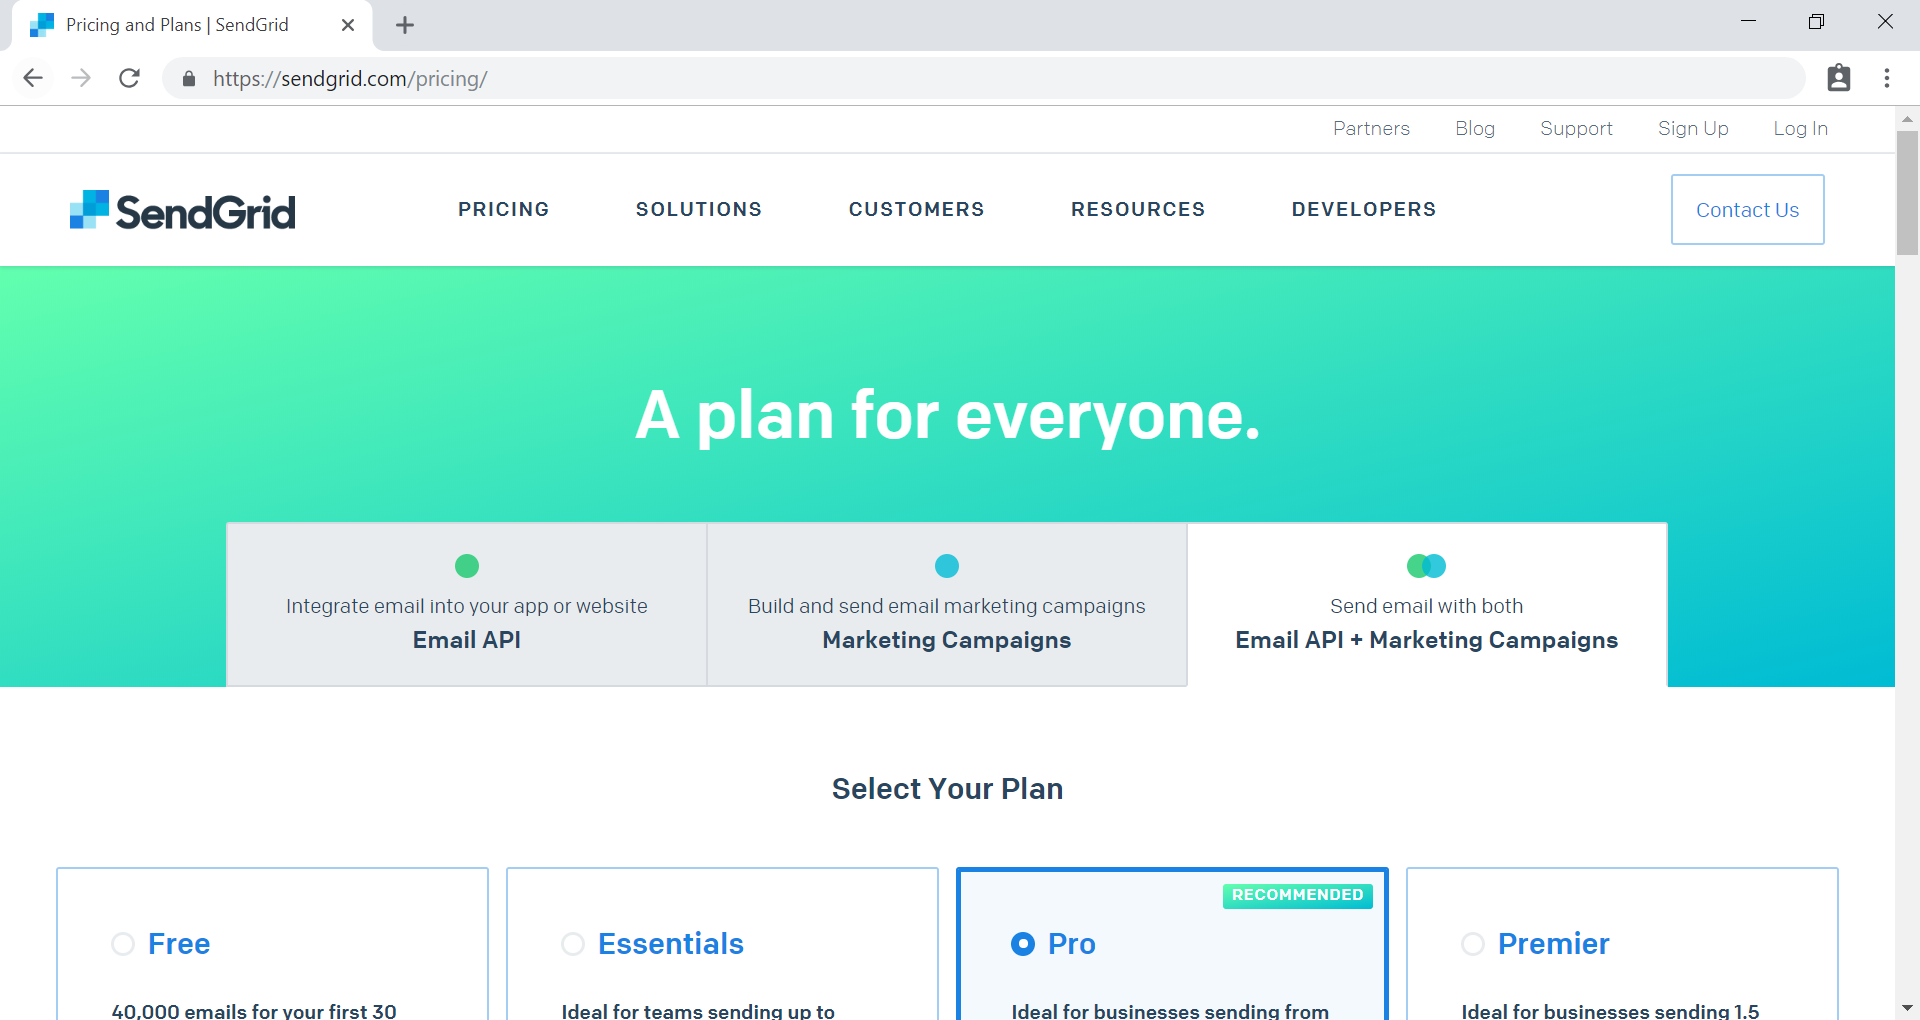
\includegraphics[width=0.6\columnwidth]{images/appendixA/SendGrid-Pricing.PNG}
	      		\caption{SendGrid Pricing and Plans page}
	      	\end{figure}
	      \end{center}
	\item Get a SendGrid API key from \href{https://app.sendgrid.com/settings/api_keys}{https://app.sendgrid.com/settings/api\_keys}
	      \begin{center}
	      	\begin{figure}[H]
	      		\centering
	      		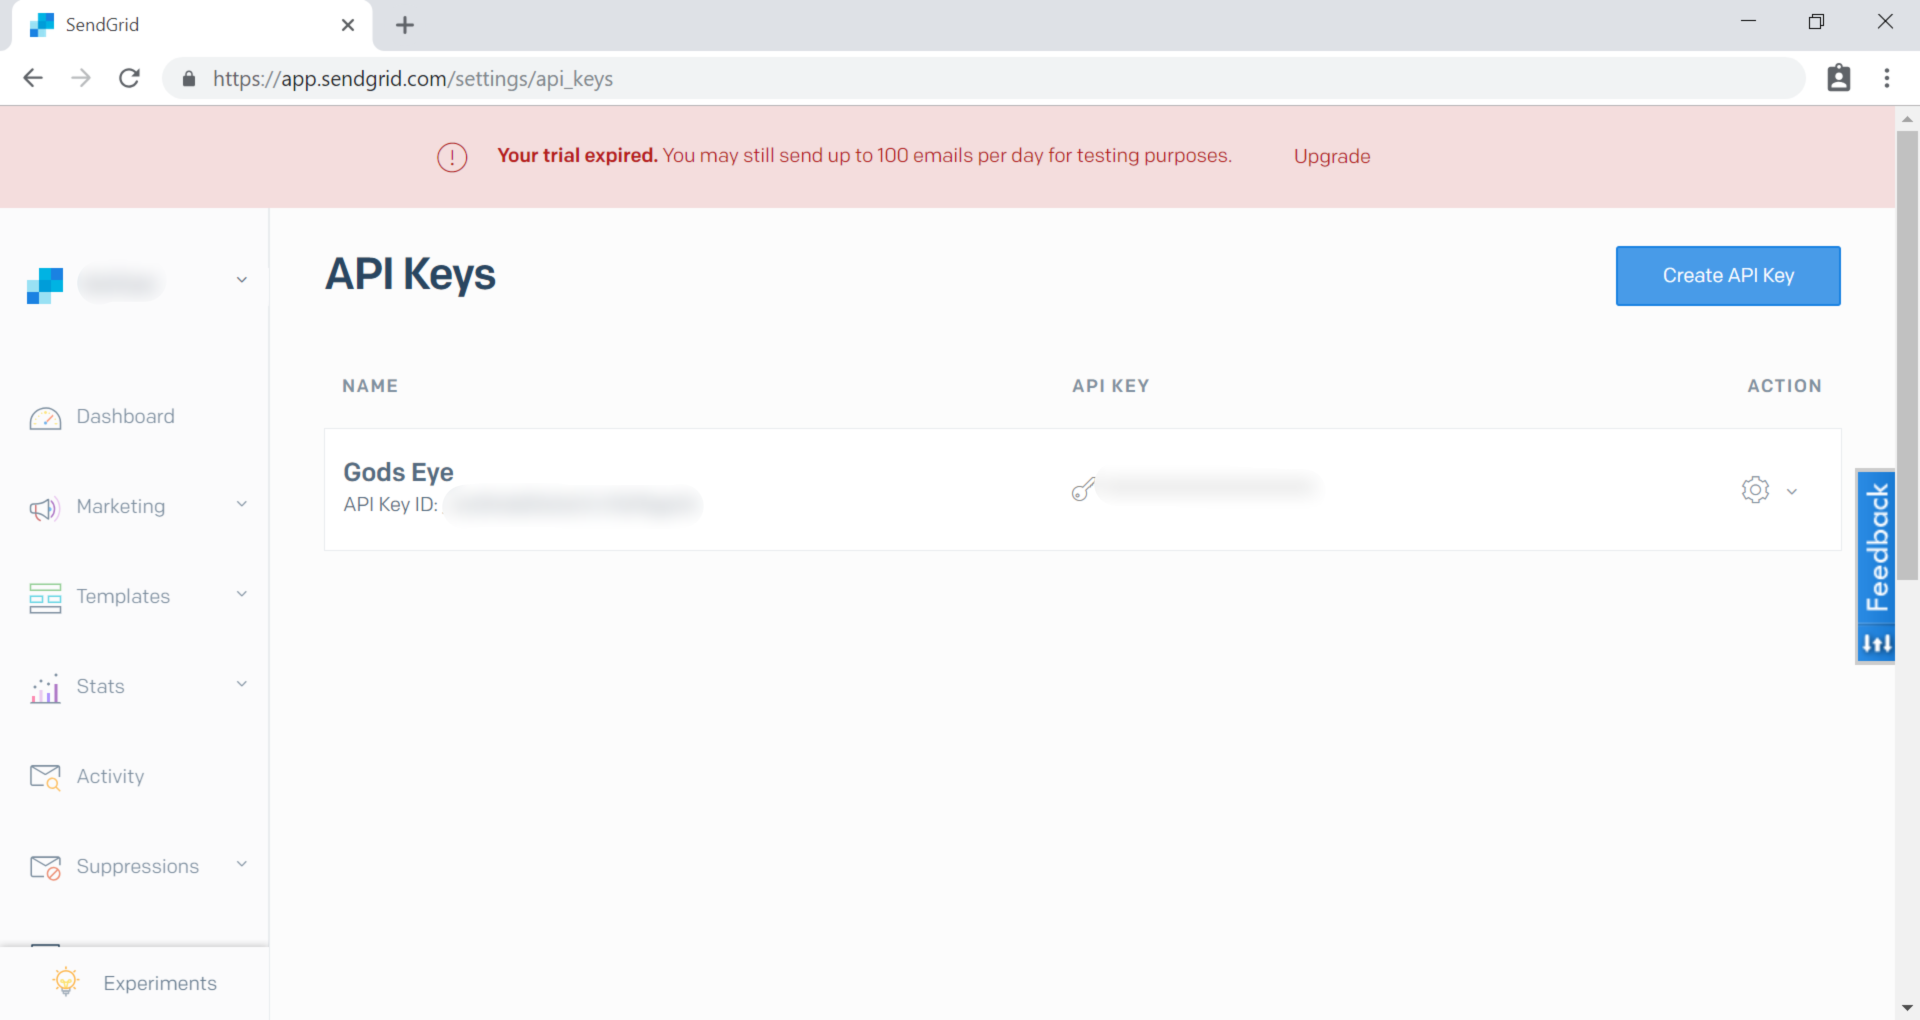
\includegraphics[width=0.6\columnwidth]{images/appendixA/SendGrid-API-Keys.png}
	      		\caption{SendGrid dashboard: API Keys}
	      	\end{figure}
	      \end{center}
	\item Follow the instruction from The Official SendGrid Led, Community Driven Node.js API Library: \href{https://github.com/sendgrid/sendgrid-nodejs}{https://github.com/sendgrid/sendgrid-nodejs}
	      \begin{center}
	      	\begin{figure}[H]
	      		\centering
	      		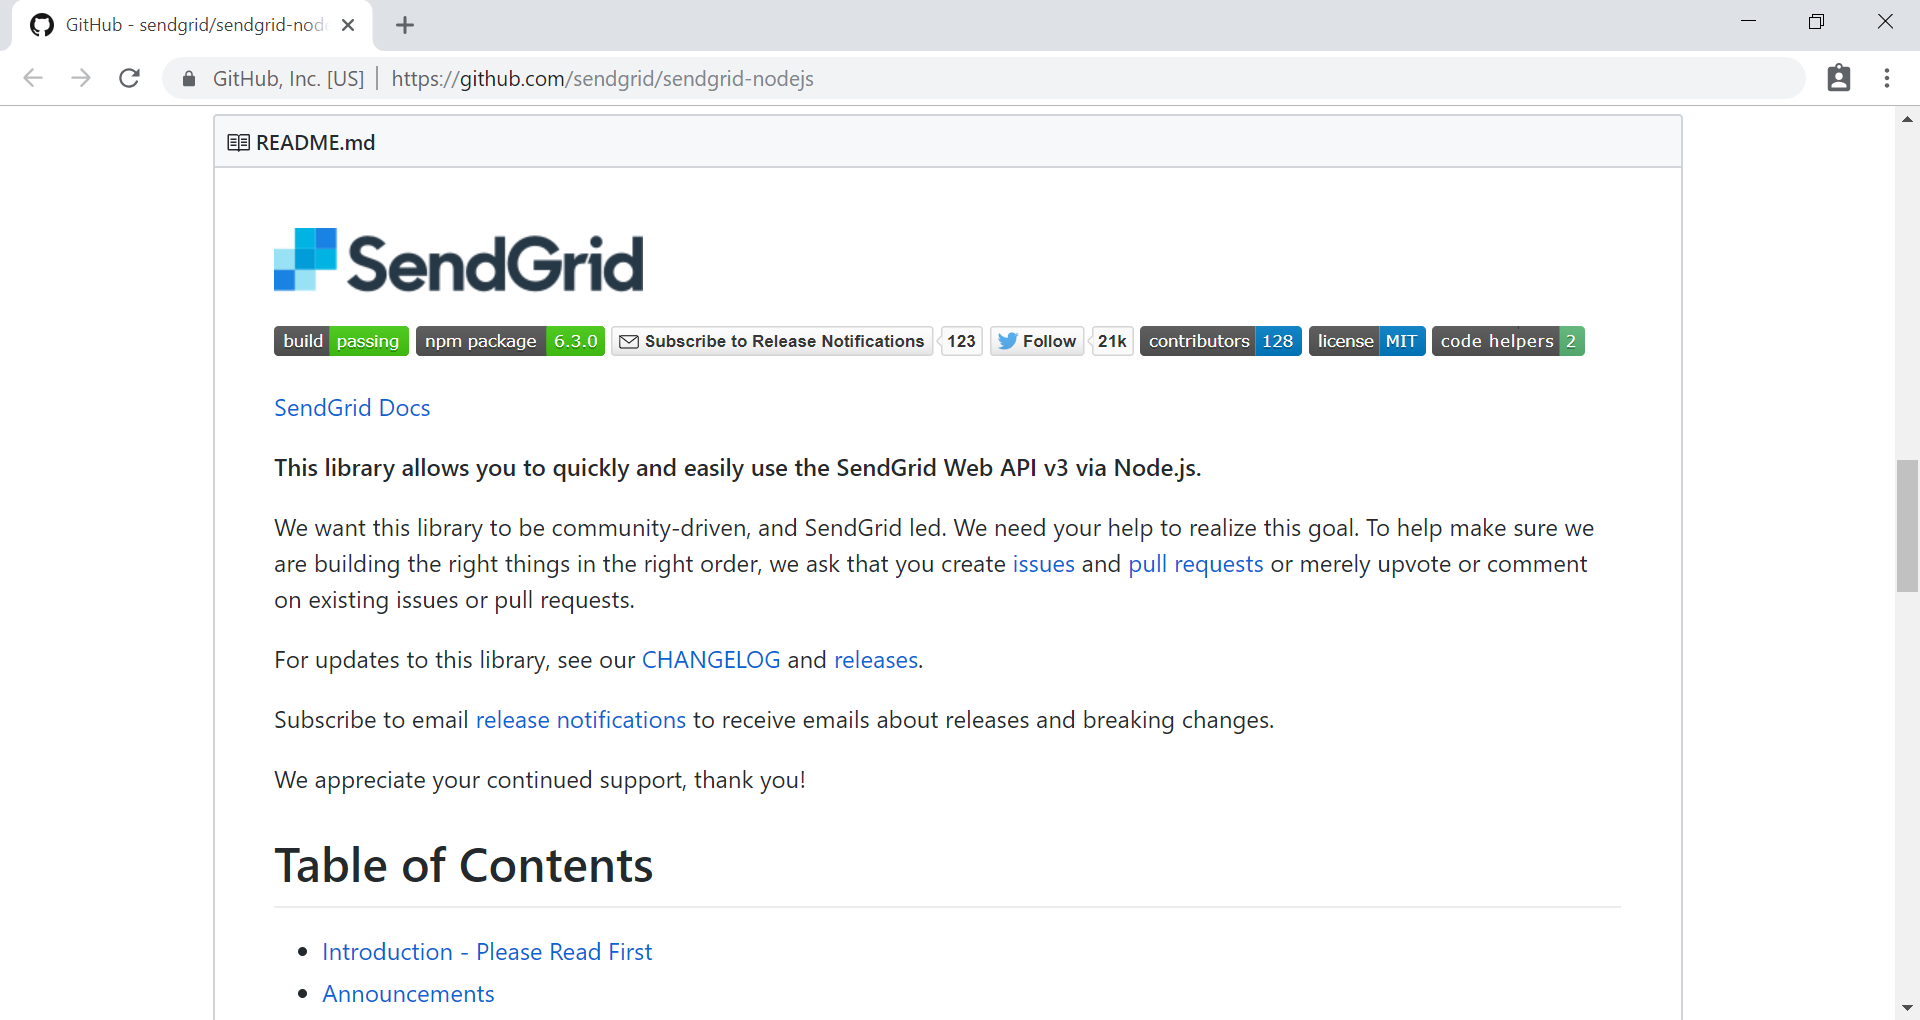
\includegraphics[width=0.6\columnwidth]{images/appendixA/SendGrid-Nodejs-Library.PNG}
	      		\caption{SendGrid Web API v3 for Node.js}
	      	\end{figure}
	      \end{center}
\end{enumerate}

\tocless\subsection{Google Maps API: Places Library}
\begin{enumerate}
	\item Follow this tutorial (\href{https://developers.google.com/maps/documentation/javascript/tutorial}{https://developers.google.com/maps/documentation/javascript/tutorial}) to integrate Google Maps JavaScript API
	      \begin{center}
	      	\begin{figure}[H]
	      		\centering
	      		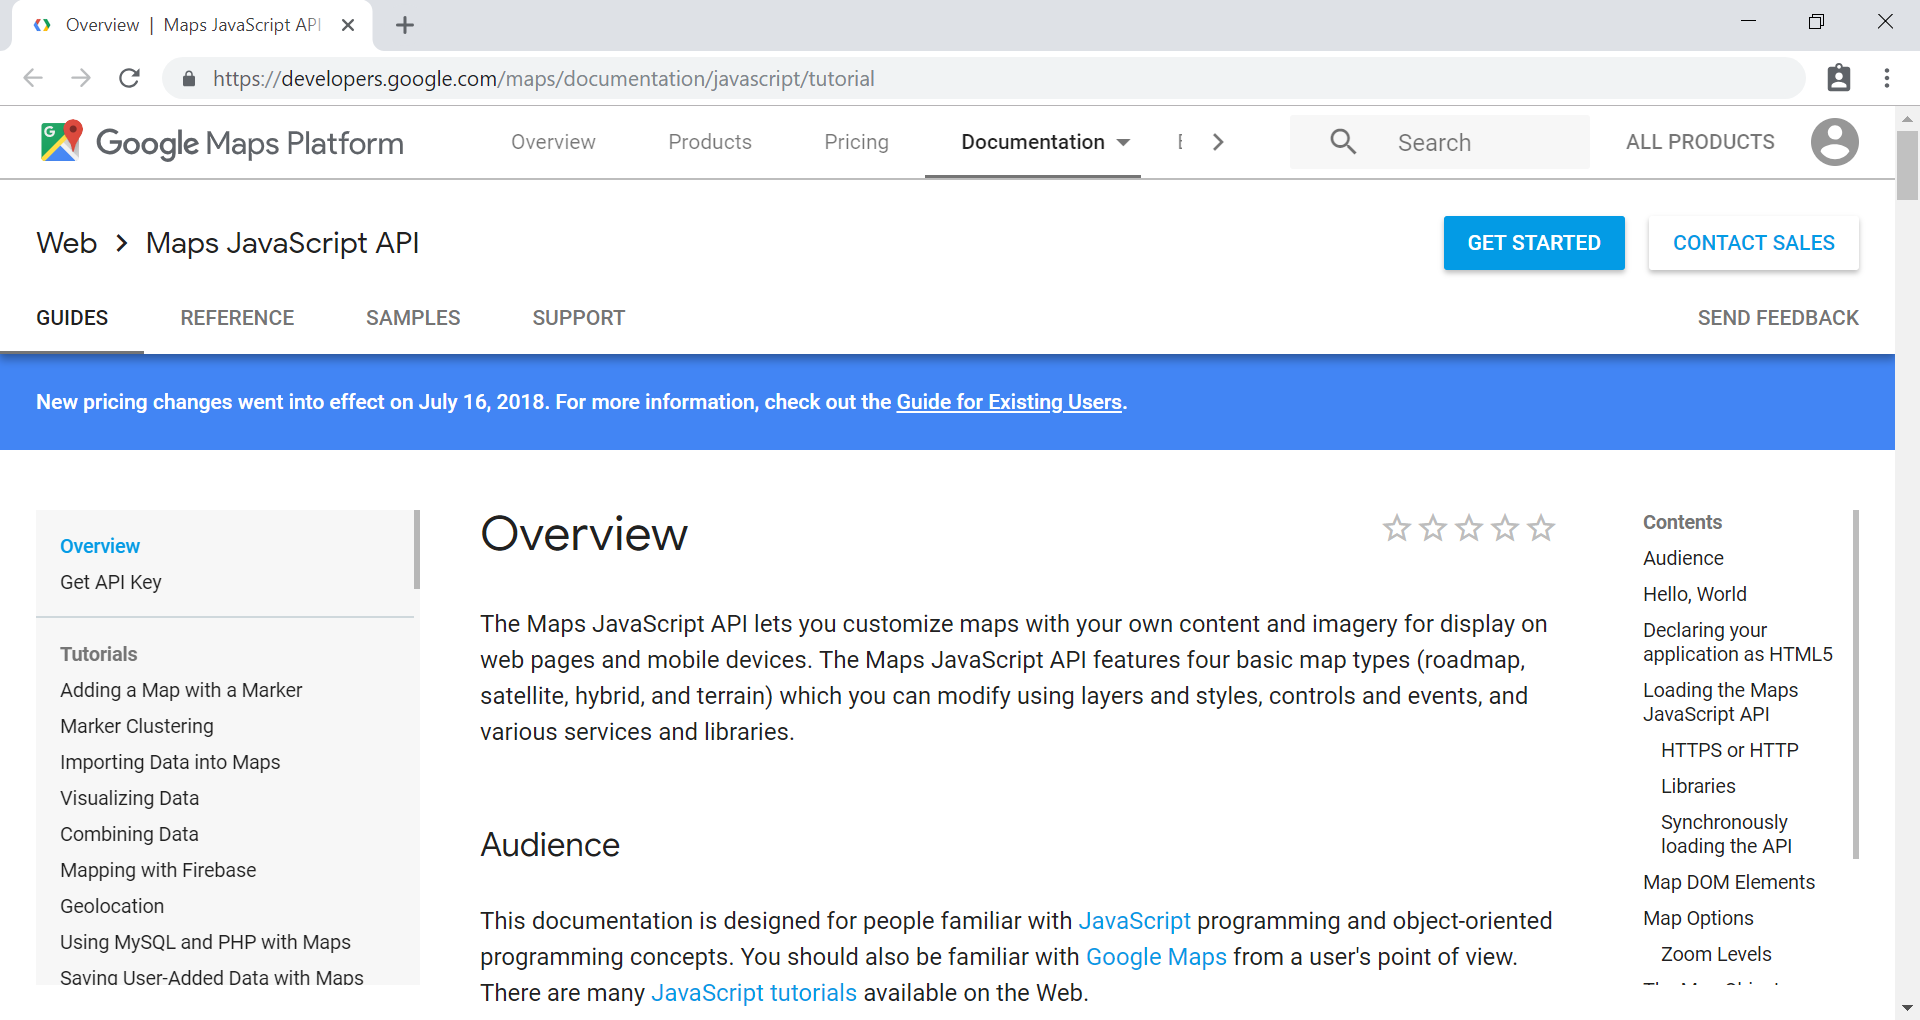
\includegraphics[width=0.6\columnwidth]{images/appendixA/Google-Maps-Tutorial.PNG}
	      		\caption{Google Maps JavaScript API Documentation}
	      	\end{figure}
	      \end{center}
	\item Get a Google Maps API key from \href{https://developers.google.com/maps/documentation/javascript/get-api-key}{https://developers.google.com/maps/documentation/javascript/get-api-key}
	      \begin{center}
	      	\begin{figure}[H]
	      		\centering
	      		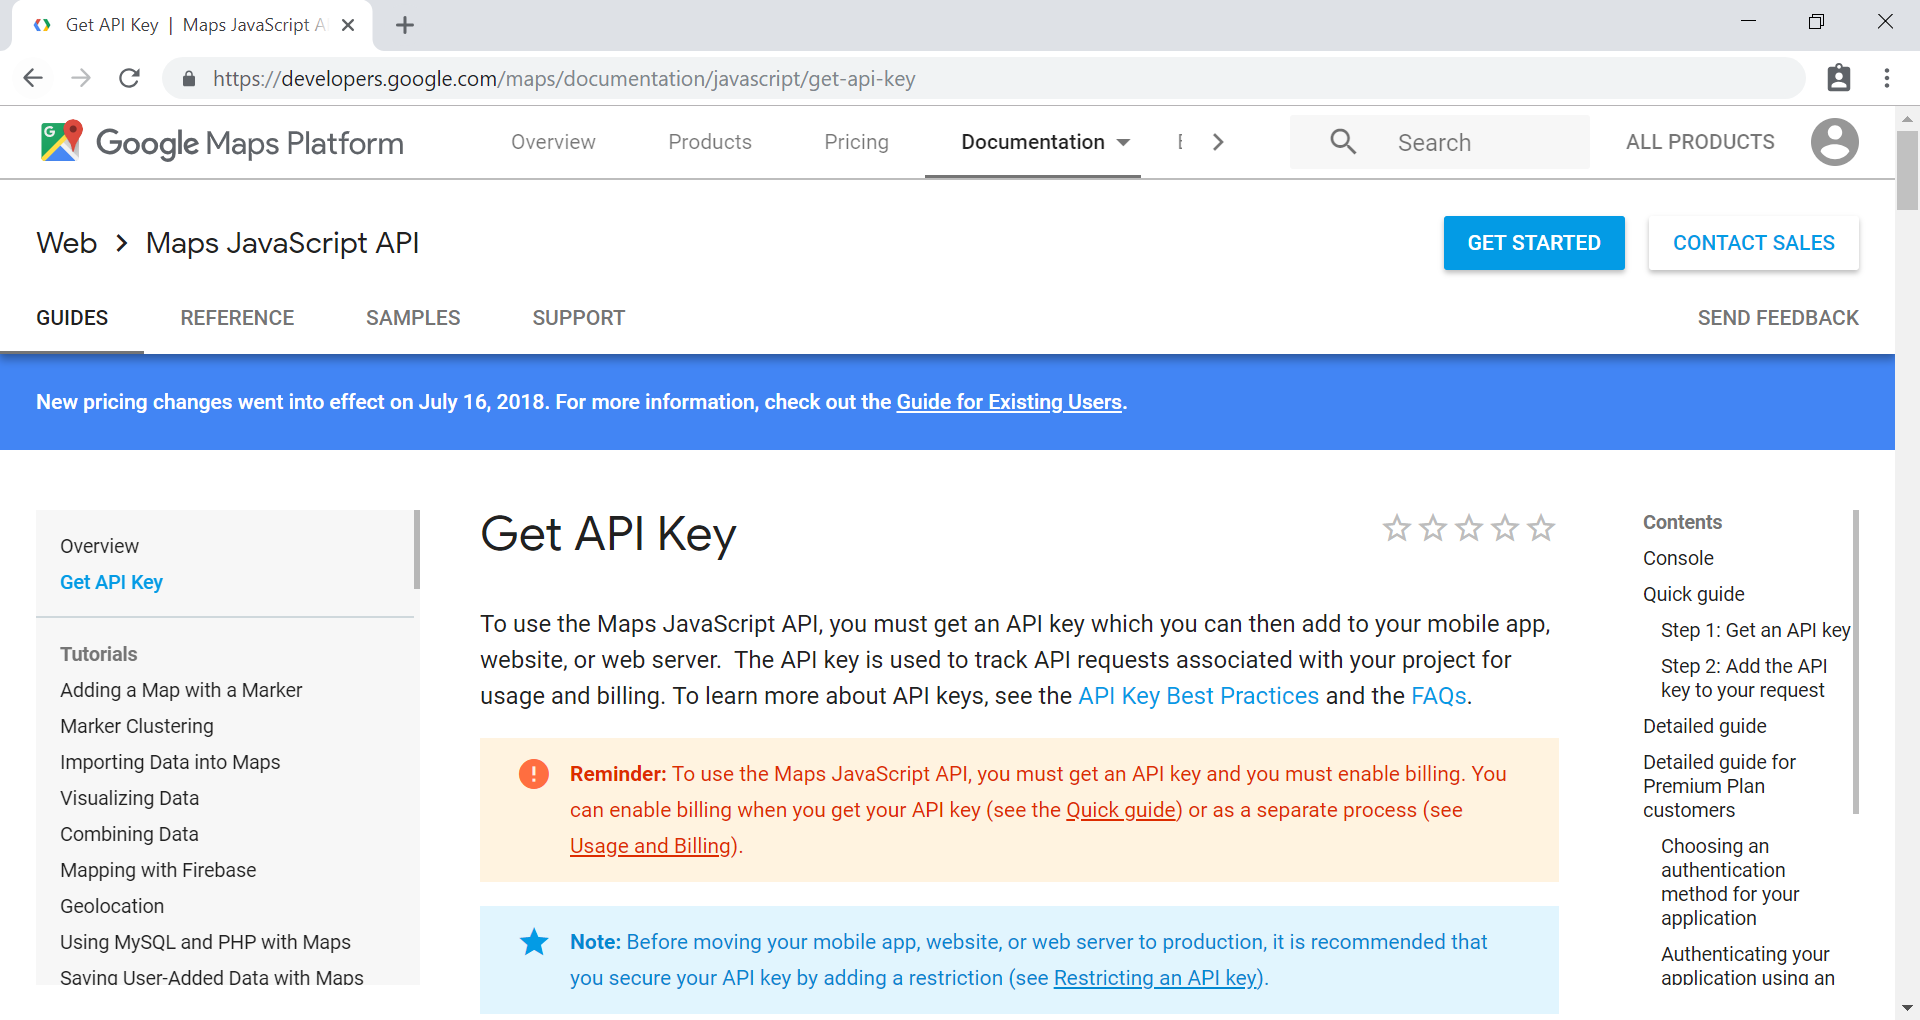
\includegraphics[width=0.6\columnwidth]{images/appendixA/Google-Maps-API-Keys.PNG}
	      		\caption{Google Maps JavaScript API Documentation: Get API Key}
	      	\end{figure}
	      \end{center}
	\item Access \href{https://developers.google.com/maps/documentation/javascript/places}{https://developers.google.com/maps/documentation/javascript/places} for more detail about Places Library
	      \begin{center}
	      	\begin{figure}[H]
	      		\centering
	      		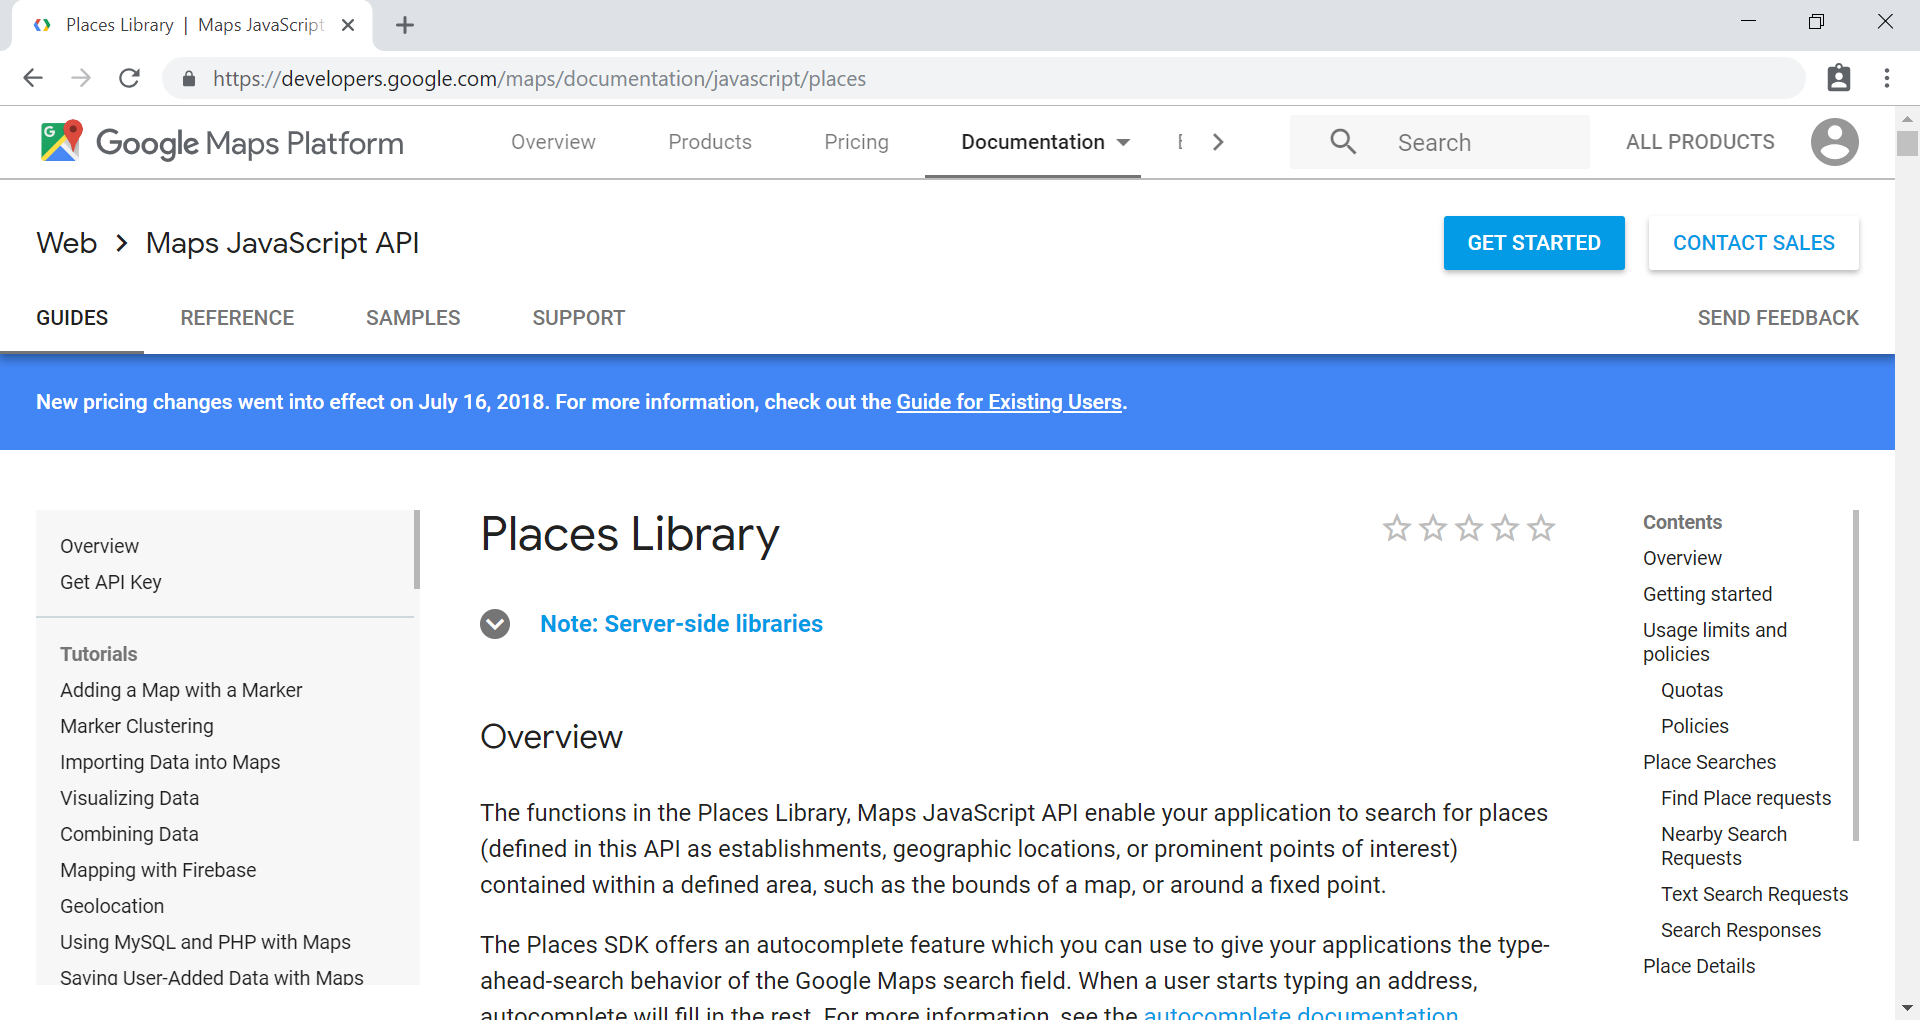
\includegraphics[width=0.6\columnwidth]{images/appendixA/Google-Maps-Places-Library.PNG}
	      		\caption{Google Maps JavaScript API Documentation: Places Library}
	      	\end{figure}
	      \end{center}
\end{enumerate}

\tocless\subsection{Google OAuth 2.0 Authentication}
\begin{enumerate}
	\item Follow this documentation (\href{http://www.passportjs.org/docs/google#oauth-2-0}{http://www.passportjs.org/docs/google\#oauth-2-0}) to integrate Google OAuth 2.0 Authentication
	      \begin{center}
	      	\begin{figure}[H]
	      		\centering
	      		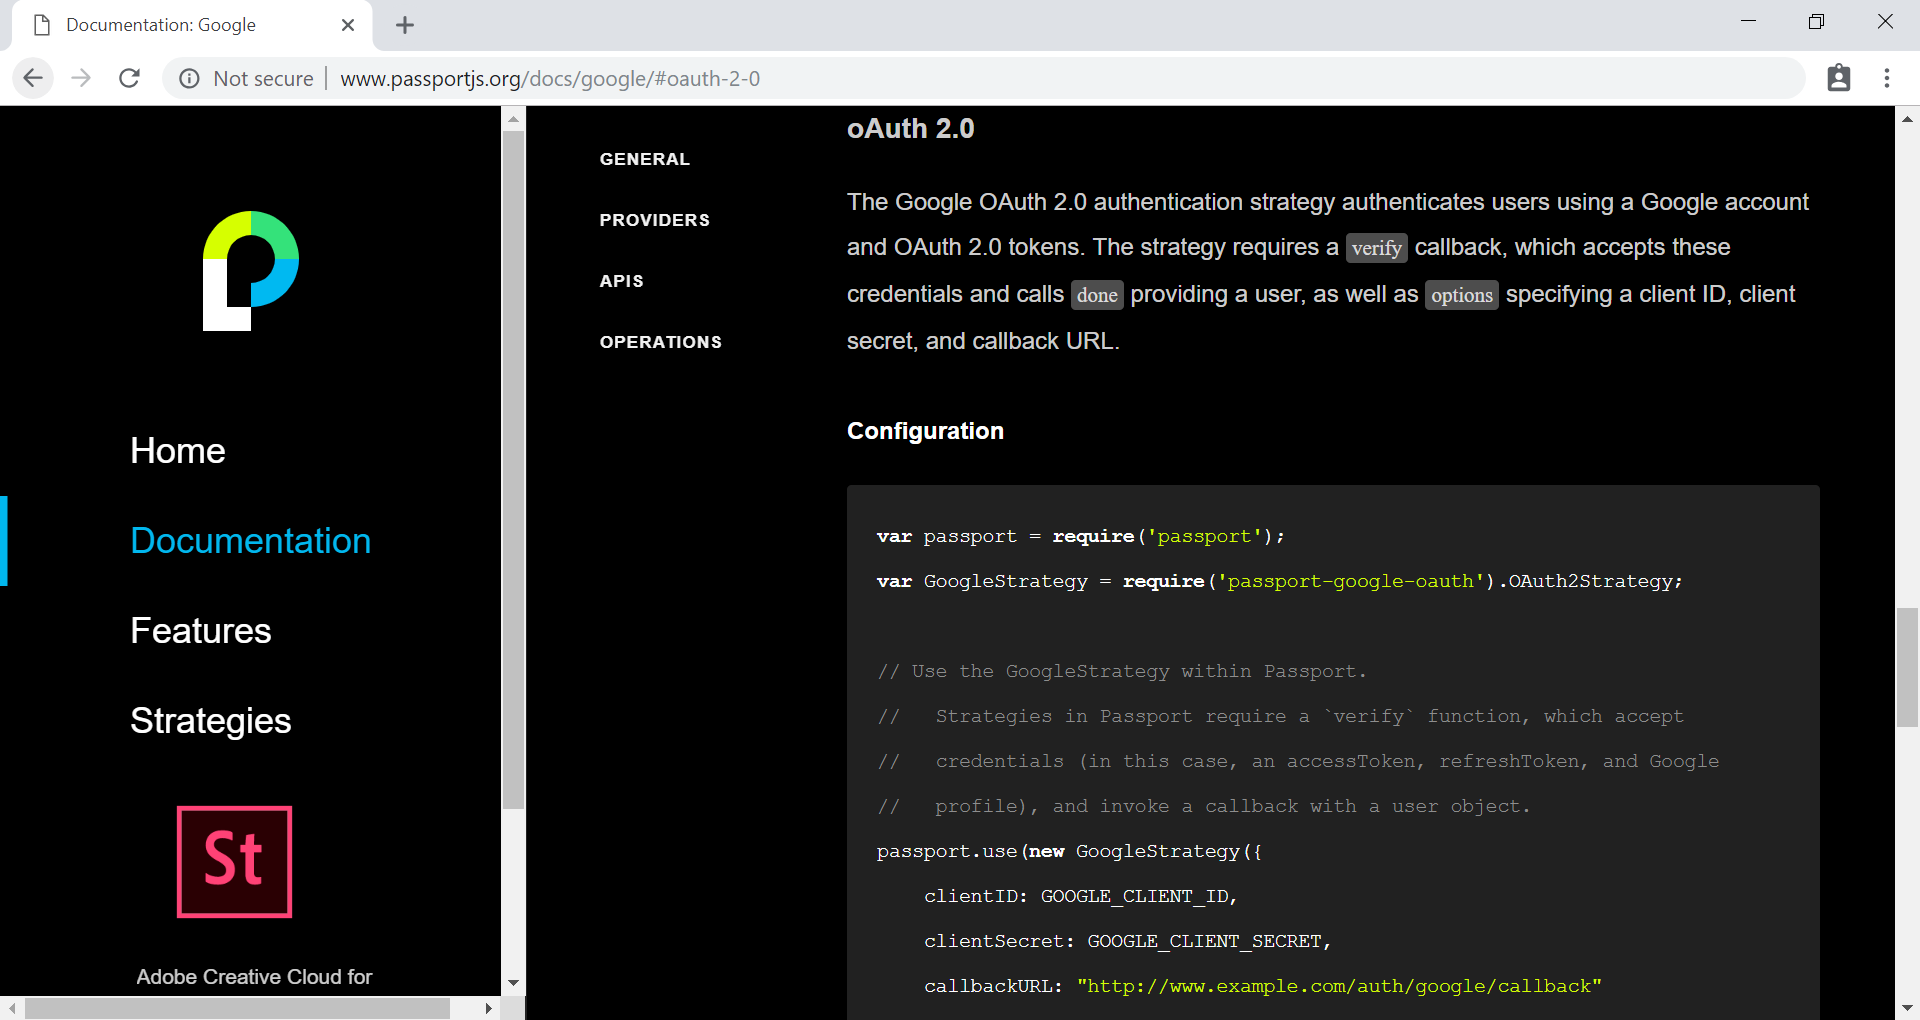
\includegraphics[width=0.6\columnwidth]{images/appendixA/Google-OAuth-Passport.PNG}
	      		\caption{Passport: Google OAuth 2.0 Authentication documentation}
	      	\end{figure}
	      \end{center}
	\item Follow this guide (\href{https://developers.google.com/adwords/api/docs/guides/authentication#webapp}{https://developers.google.com/adwords/api/docs/guides/authentication\#webapp}) to create a client ID and client secret for Google OAuth 2.0 Authentication
	      \begin{center}
	      	\begin{figure}[H]
	      		\centering
	      		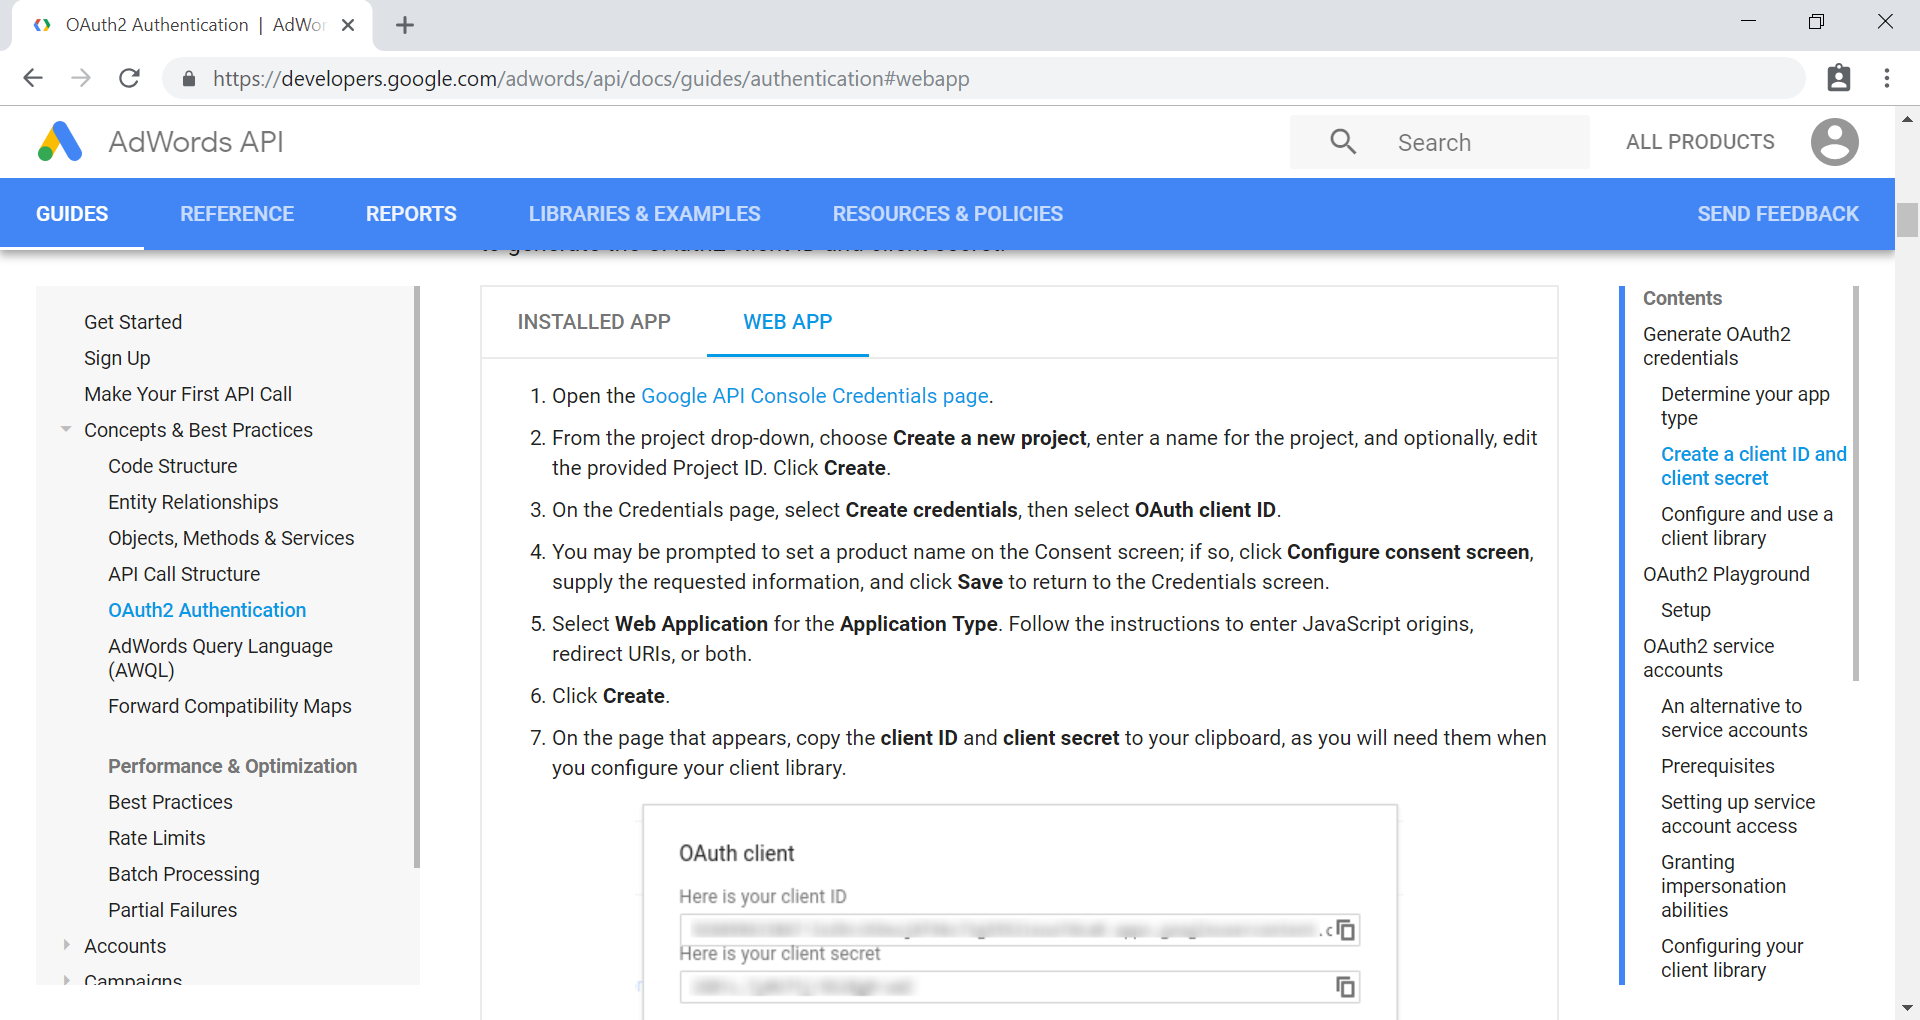
\includegraphics[width=0.6\columnwidth]{images/appendixA/Google-OAuth-Guide.PNG}
	      		\caption{Google OAuth 2.0 Authentication Guide}
	      	\end{figure}
	      \end{center}
	\item Go to Google API Console (\href{https://console.cloud.google.com/apis/dashboard}{https://console.cloud.google.com/apis/dashboard}) to manage Credentials (\href{https://console.cloud.google.com/apis/credentials}{https://console.cloud.google.com/apis/credentials}). For advanced configuration, select the just created OAuth 2.0 client ID
	      \begin{center}
	      	\begin{figure}[H]
	      		\centering
	      		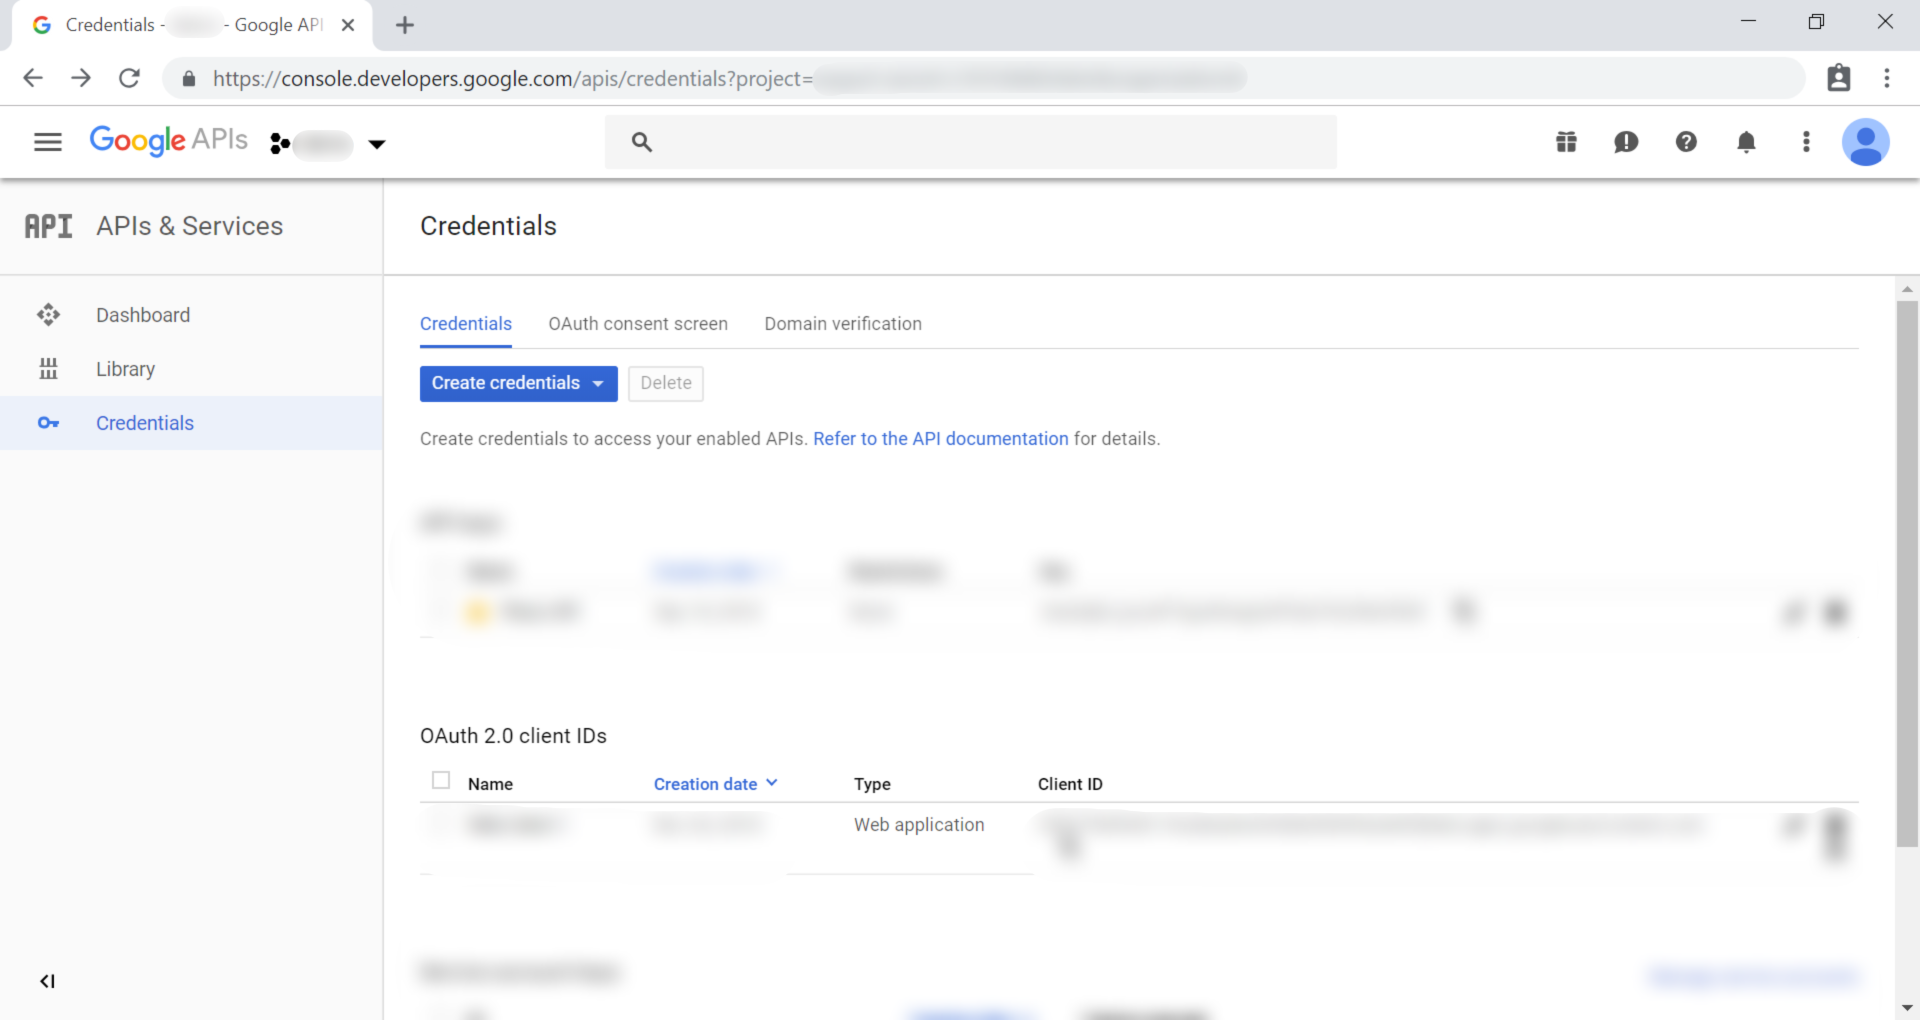
\includegraphics[width=0.6\columnwidth]{images/appendixA/Google-OAuth-Credentials.png}
	      		\caption{Google OAuth 2.0 Authentication: Credentials}
	      	\end{figure}
	      \end{center}
	      \begin{center}
	      	\begin{figure}[H]
	      		\centering
	      		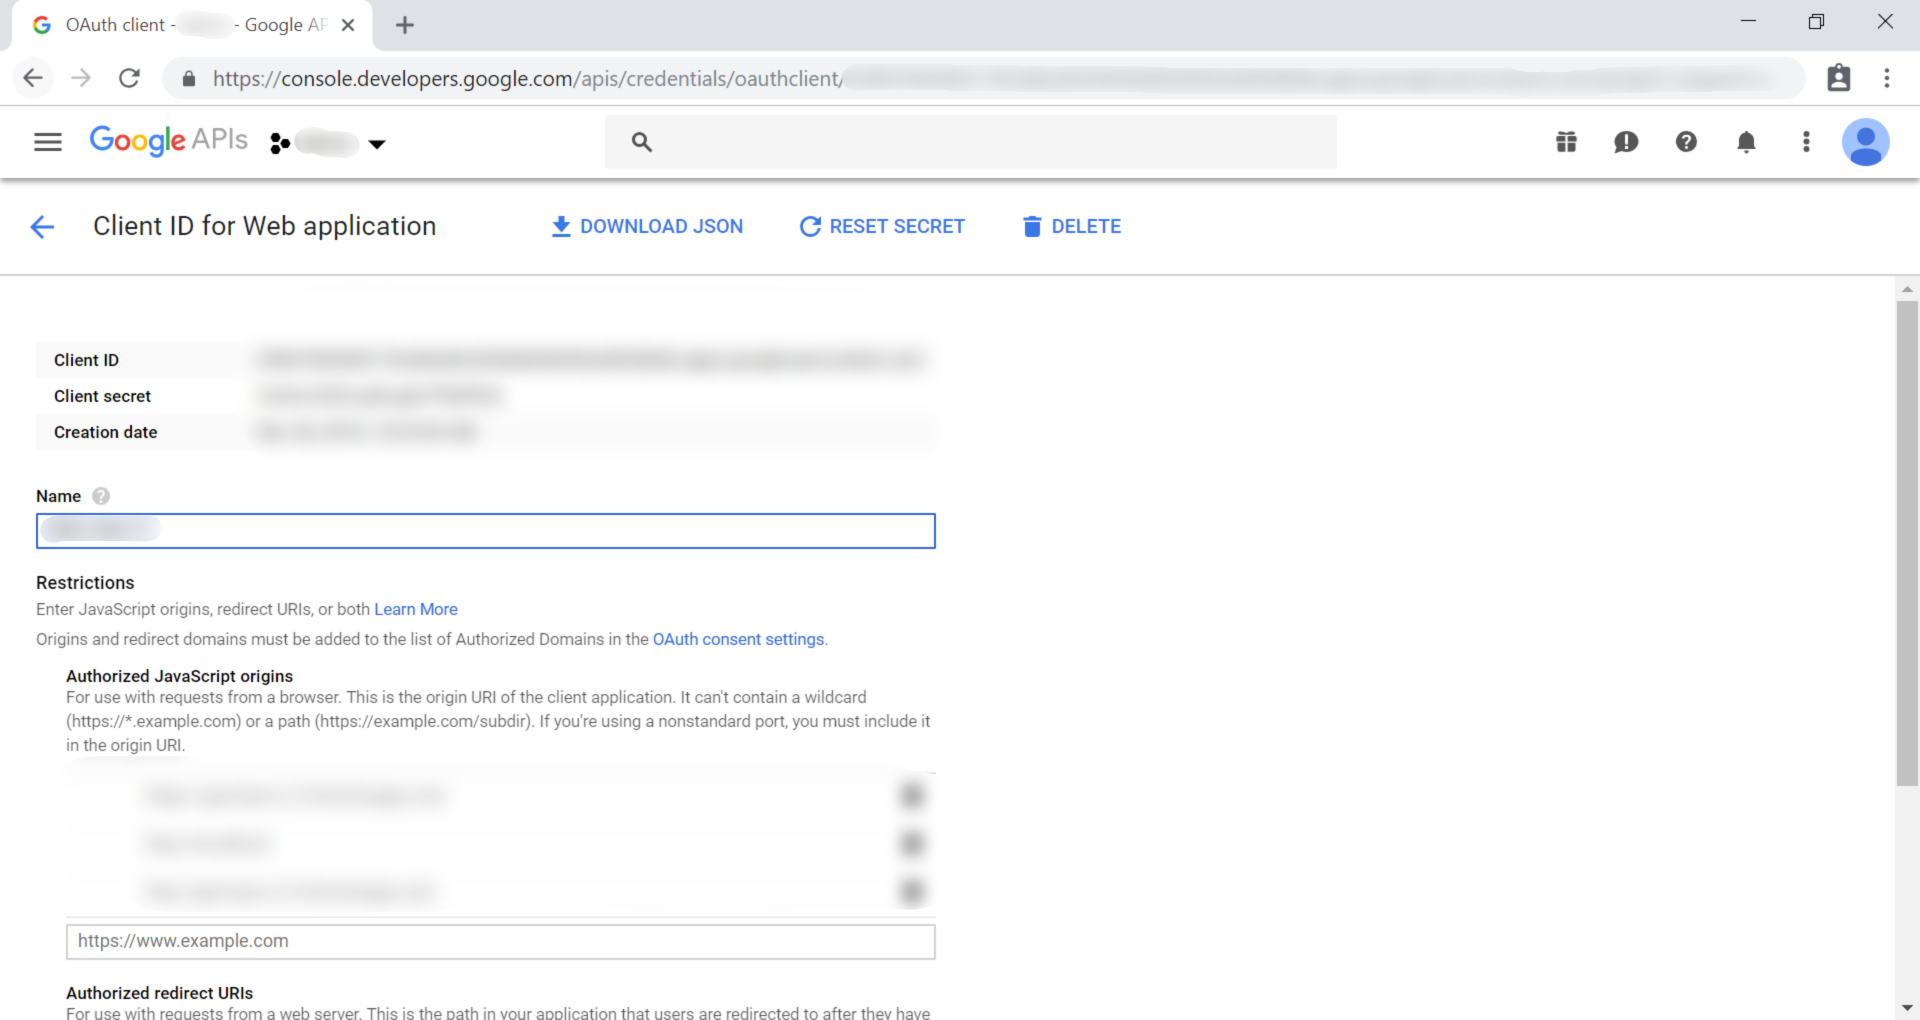
\includegraphics[width=0.6\columnwidth]{images/appendixA/Google-OAuth-Settings.png}
	      		\caption{Google OAuth 2.0 Authentication: OAuth Client Settings}
	      	\end{figure}
	      \end{center}
\end{enumerate}
\section{Source code}
\begin{enumerate}
\item Clone or download this thesis source code from this GitHub repository \href{https://github.com/dalo2903/gods-eye/}{https://github.com/dalo2903/gods-eye/}
\begin{center}
    \begin{figure}[H]
    \centering
    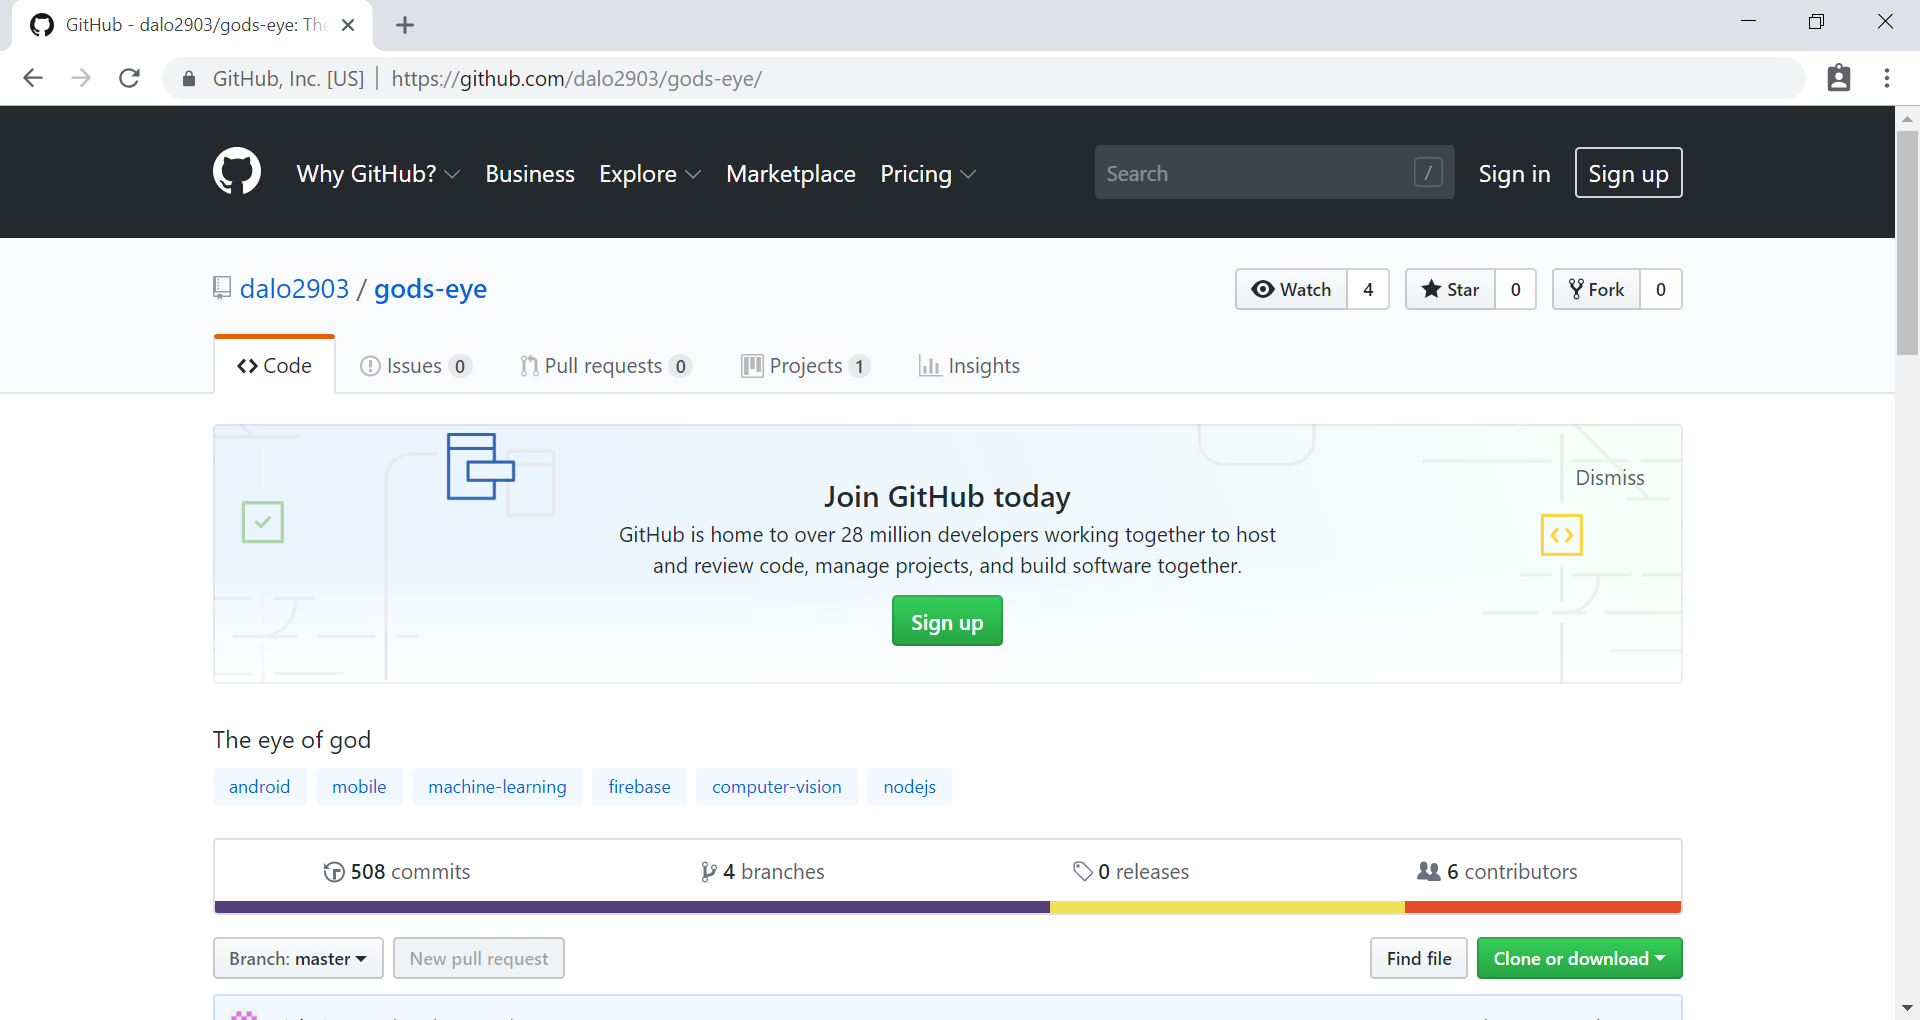
\includegraphics[width=1\columnwidth]{images/appendixA/GodsEye-GitHub.PNG}
    \caption{Thesis Source Code Repository}
    \end{figure}
\end{center}
\item Replace default environment variables (in .env and config.js) with appropriate keys from above services
\item Follow instruction in ReadMe.MD to run source code
\item Replace variables in .env file with API keys in above section
\end{enumerate}

\chapter{User manual}
\section{Verifying account}
1. Login with your account or register new account. 
\begin{center}
	\begin{figure}[H]
		\centering
		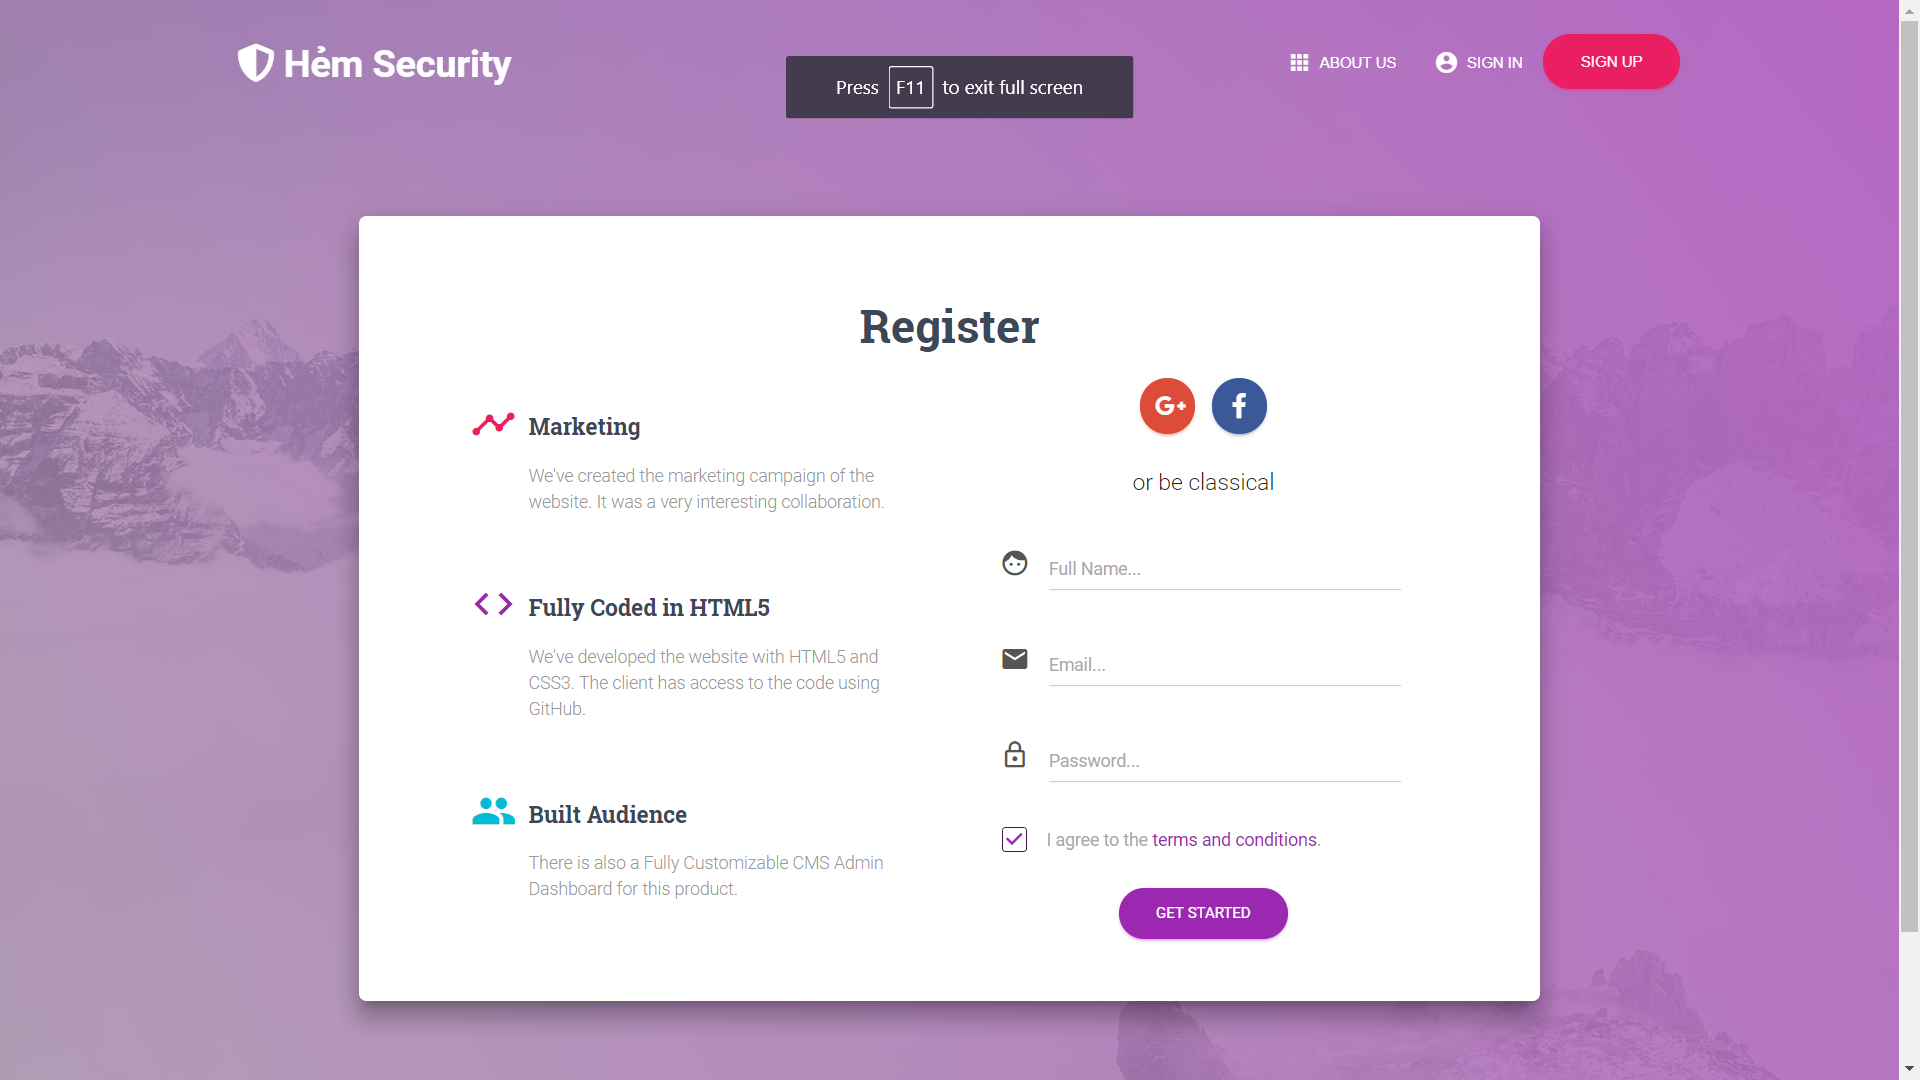
\includegraphics[width=1\columnwidth]{images/chap6/instruction1.png}
		\footcaption{Homepage}
		\label{}
	\end{figure}
\end{center}
2. Unverified account is unable to use most of the features, verify your account by clicking your name to go to your profile page
\begin{center}
	\begin{figure}[H]
		\centering
		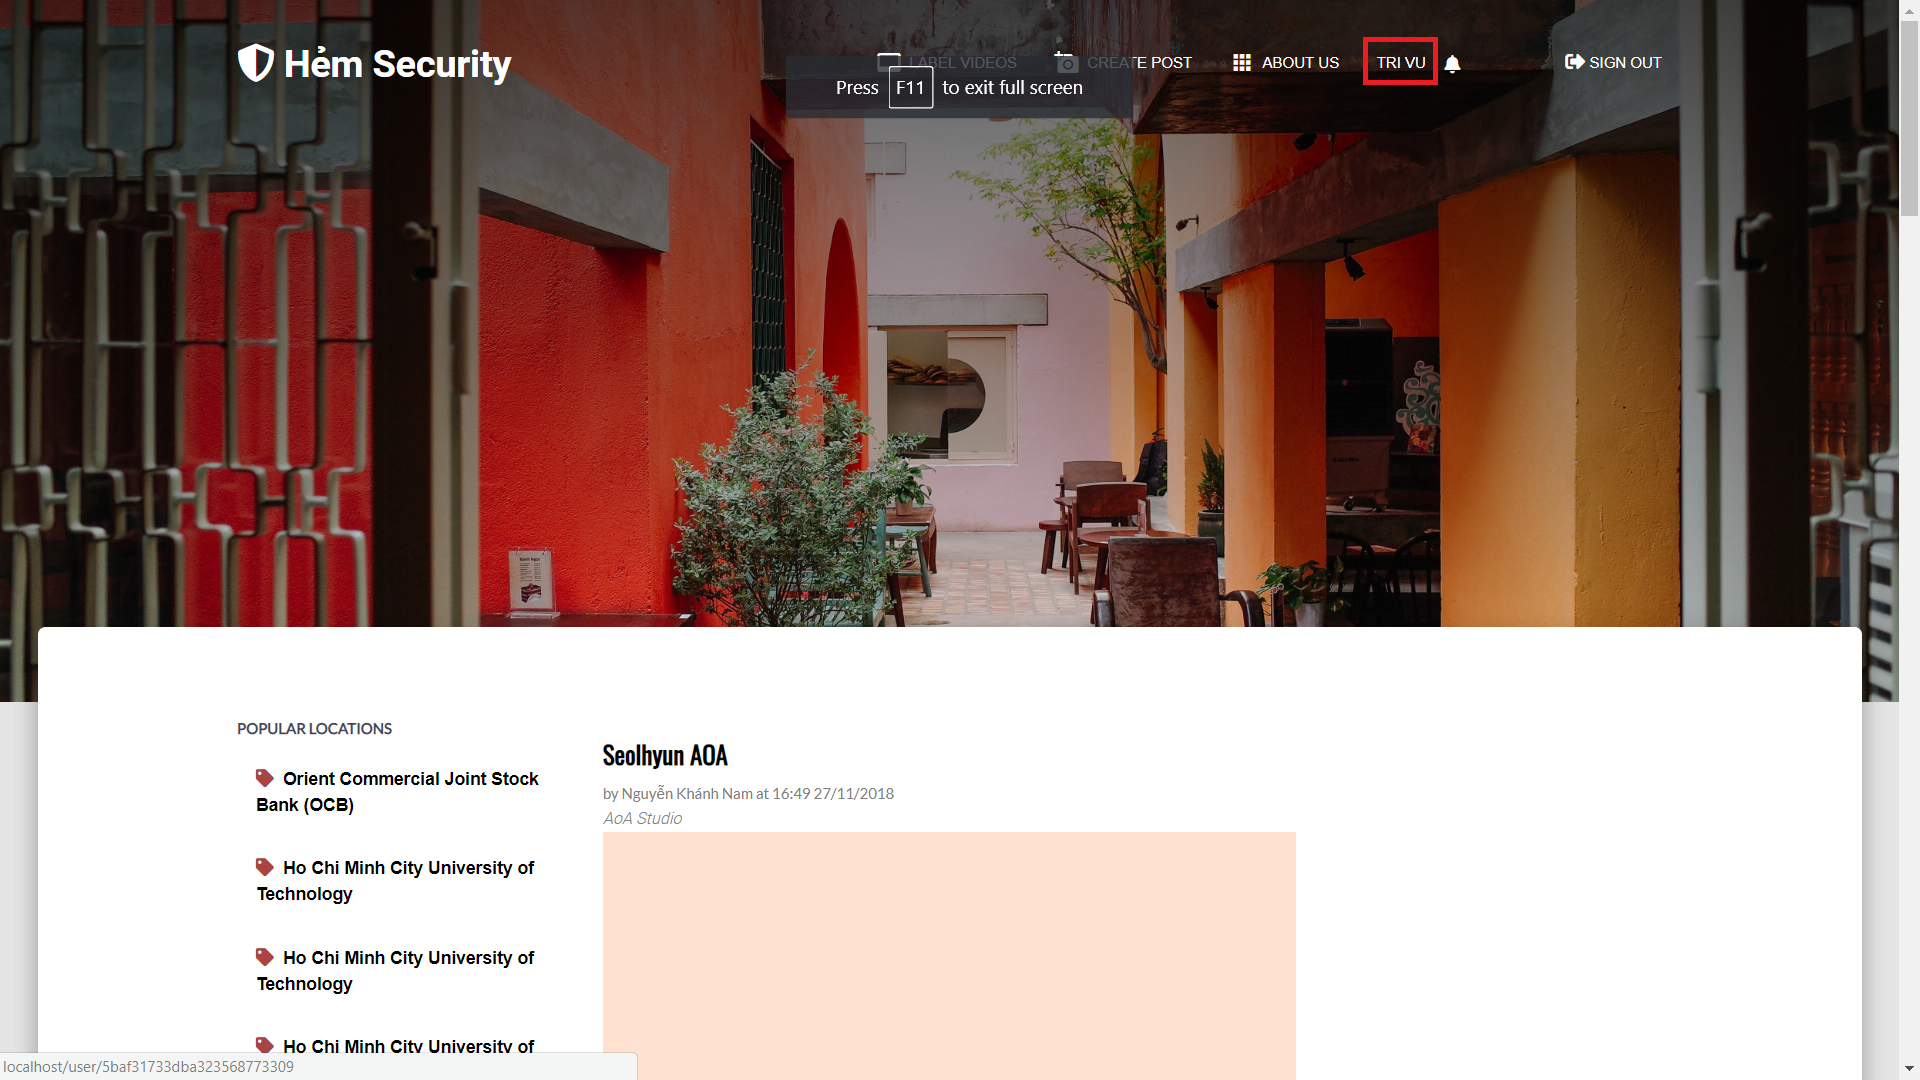
\includegraphics[width=1\columnwidth]{images/chap6/instruction2.png}
	\end{figure}
\end{center}
3. Enter your phone number to verify
\begin{center}
	\begin{figure}[H]
		\centering
		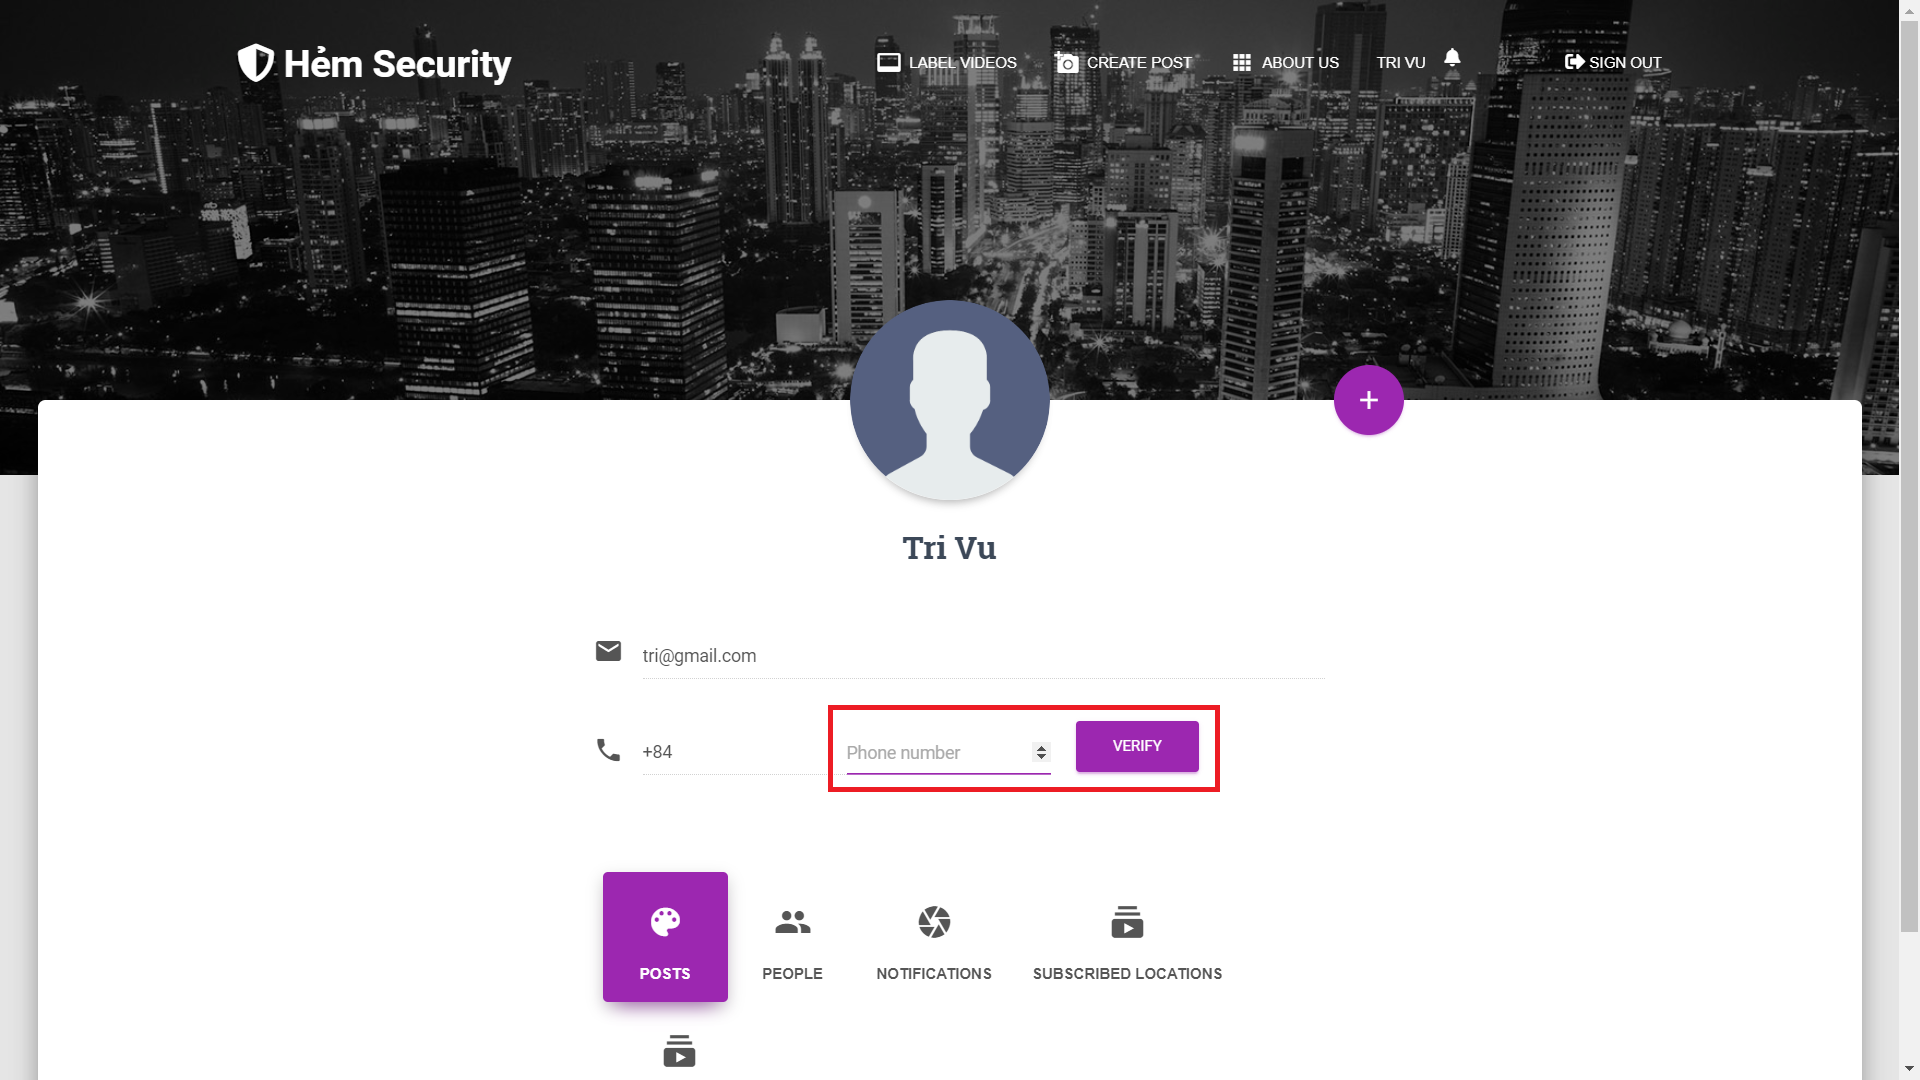
\includegraphics[width=1\columnwidth]{images/chap6/instruction3.png}
	\end{figure}
\end{center}
4. User can choose either to receive confirmation code by WhatsApp or SMS. Enter your code to finish verifying.
\begin{center}
	\begin{figure}[H]
		\centering
		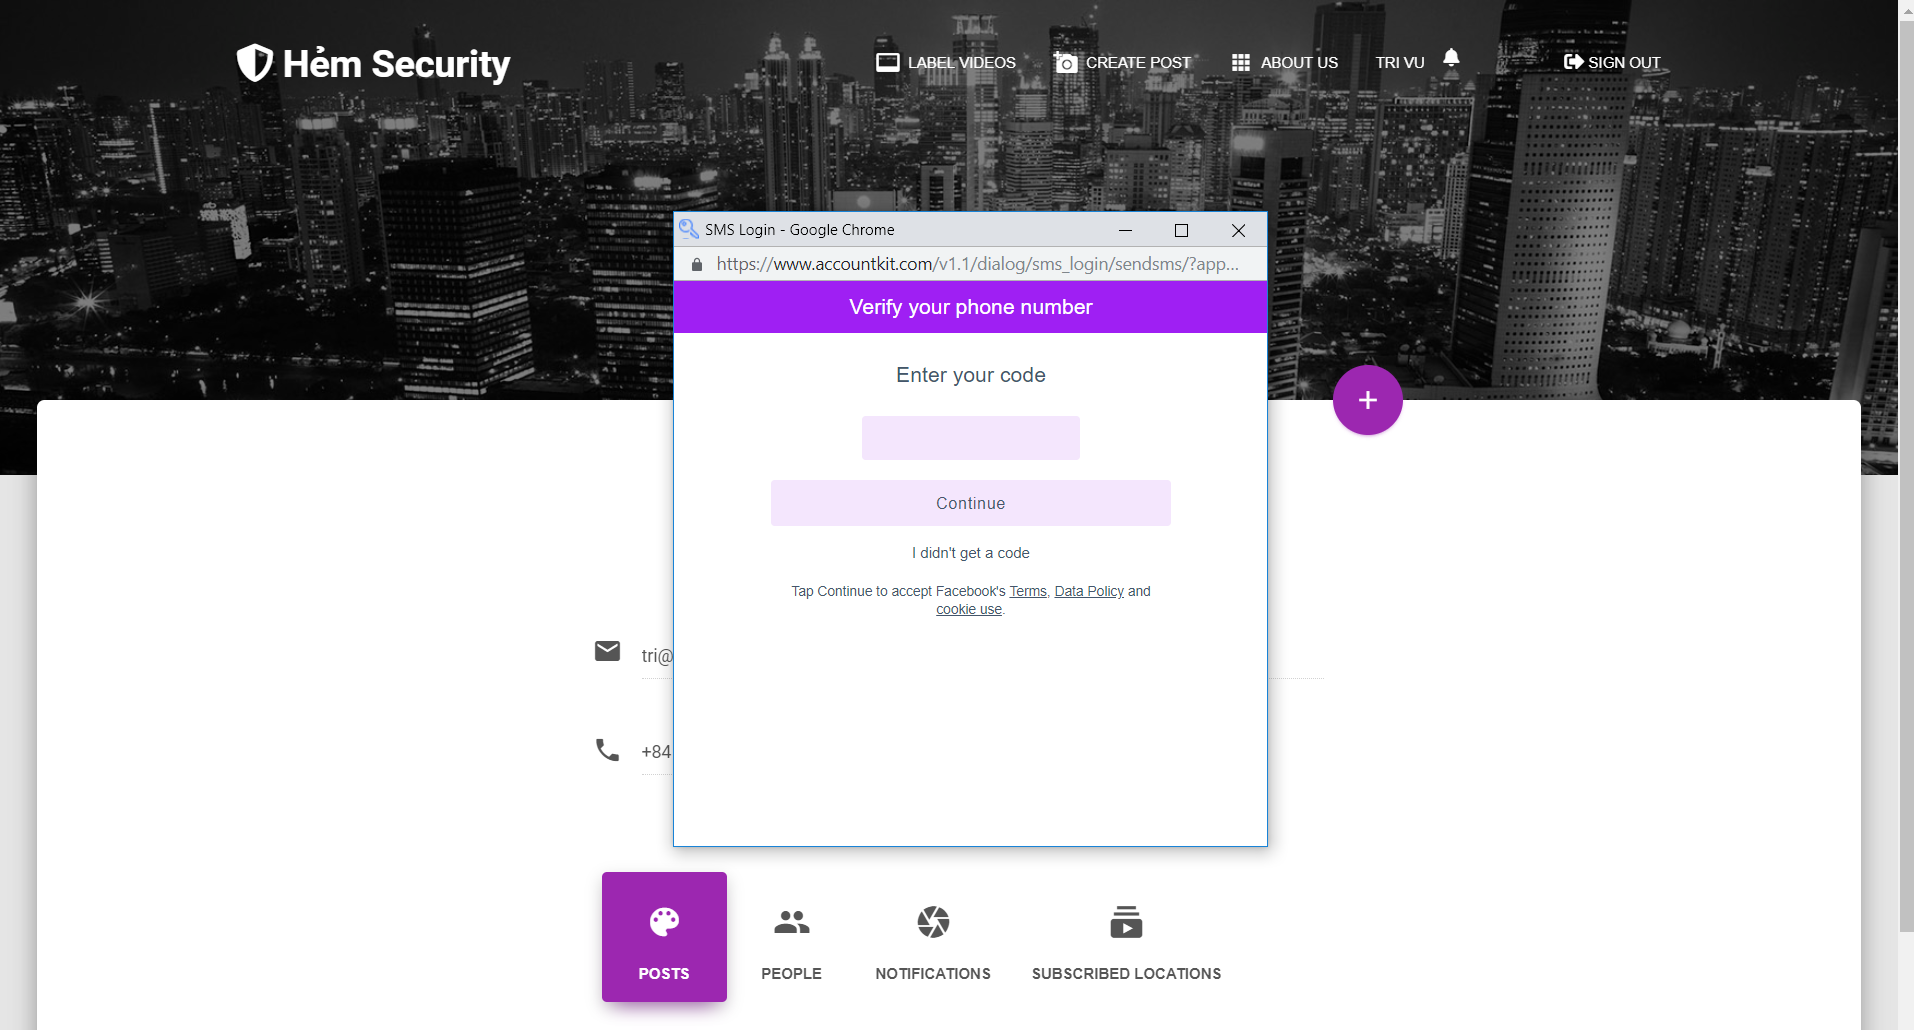
\includegraphics[width=1\columnwidth]{images/chap6/instruction4.png}
	\end{figure}
\end{center}
\section{Label video}
1. Go to "Label video" page
\begin{center}
	\begin{figure}[H]
		\centering
		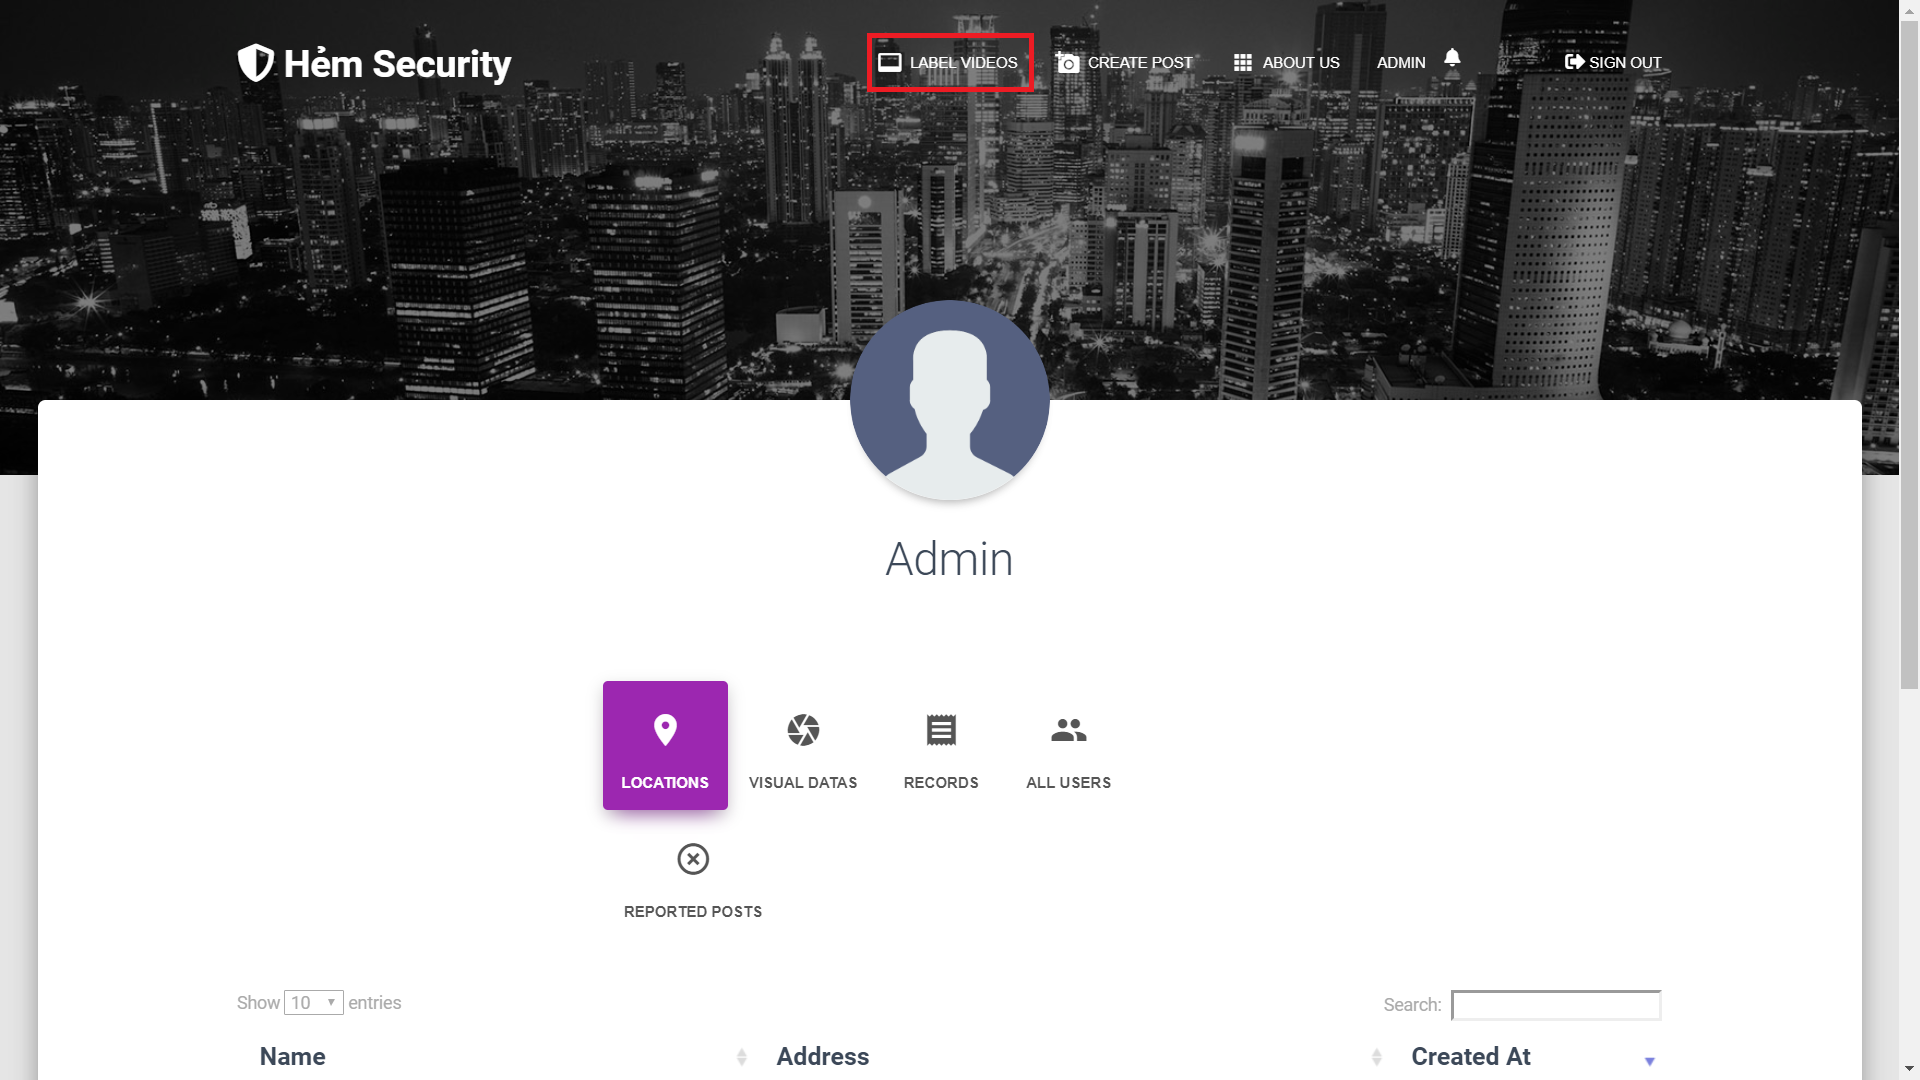
\includegraphics[width=1\columnwidth]{images/chap6/instruction5.png}
	\end{figure}
\end{center}
2. Choose either "Suspicious" or "Not suspicious". 
\begin{center}
	\begin{figure}[H]
		\centering
		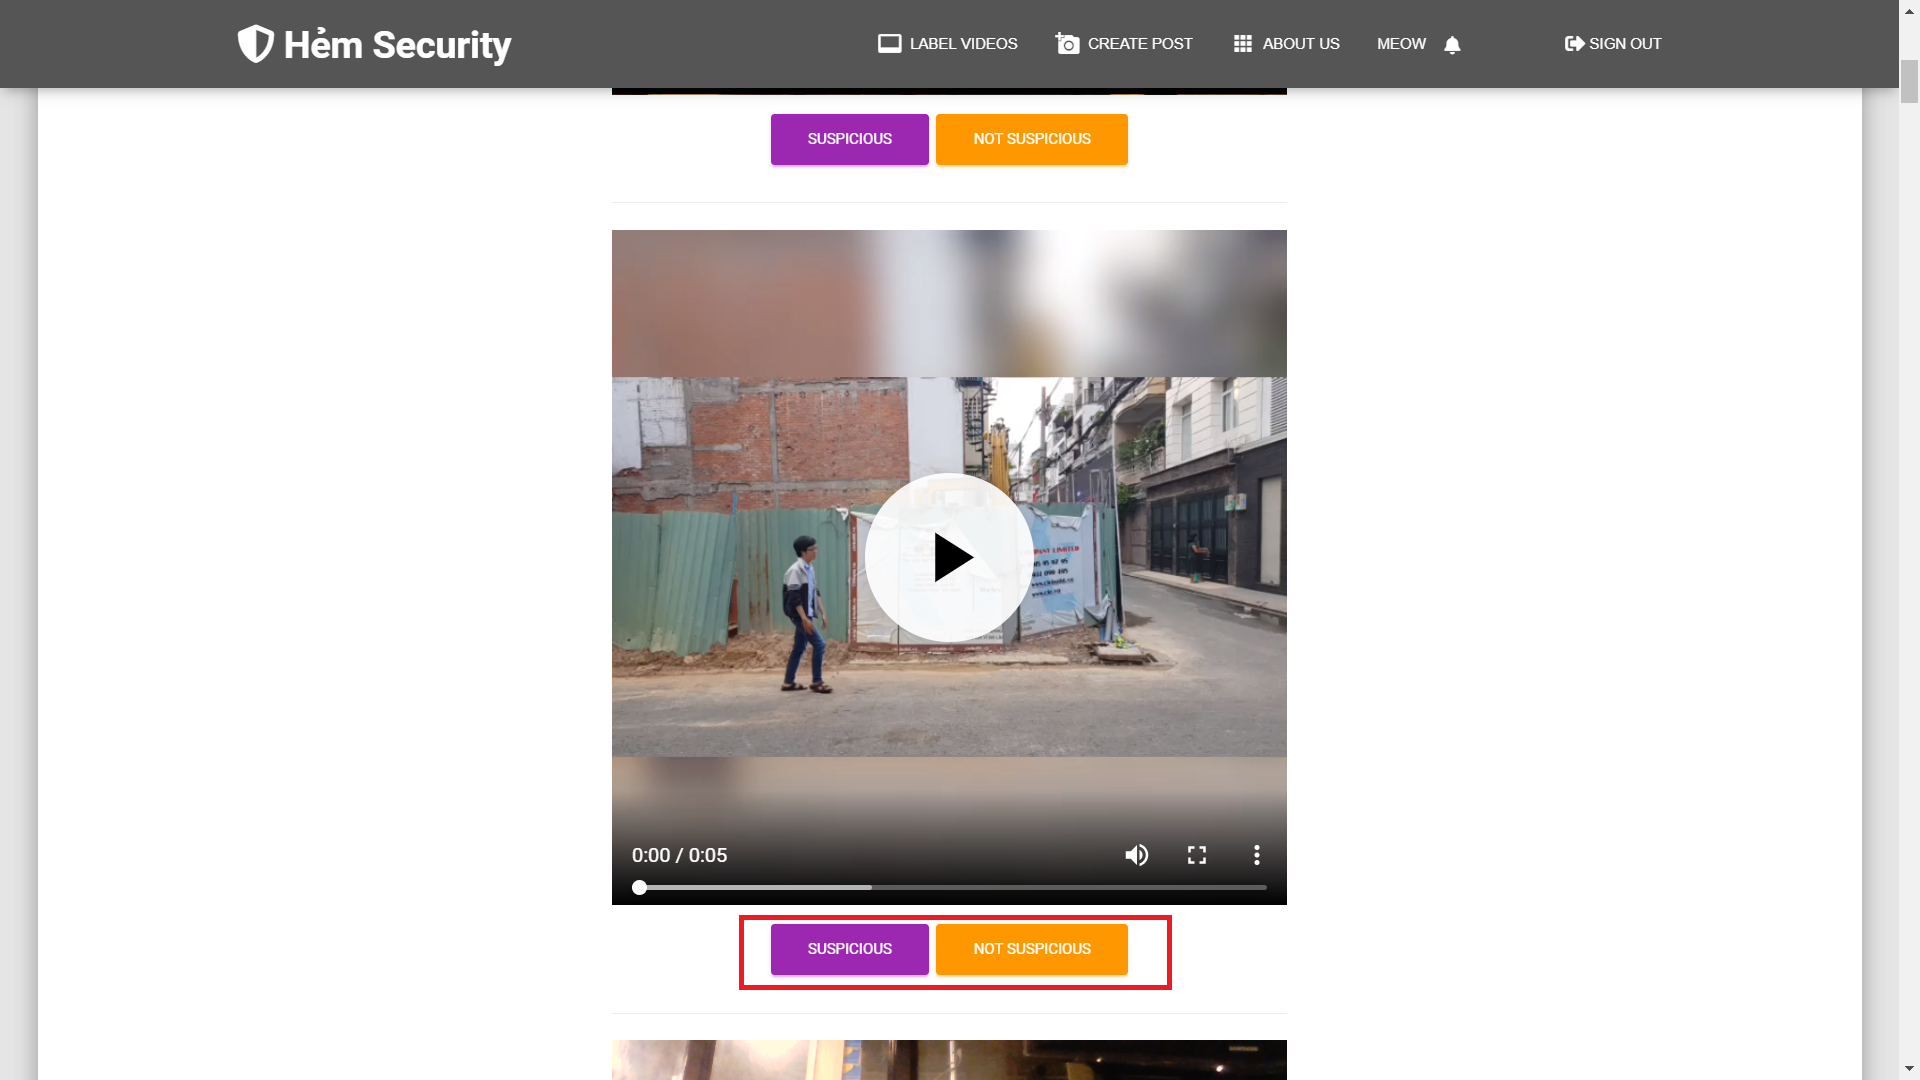
\includegraphics[width=1\columnwidth]{images/chap6/instruction6.png}
	\end{figure}
\end{center}
\section{Create post}
1. Go to "Create post" page
\begin{center}
	\begin{figure}[H]
		\centering
		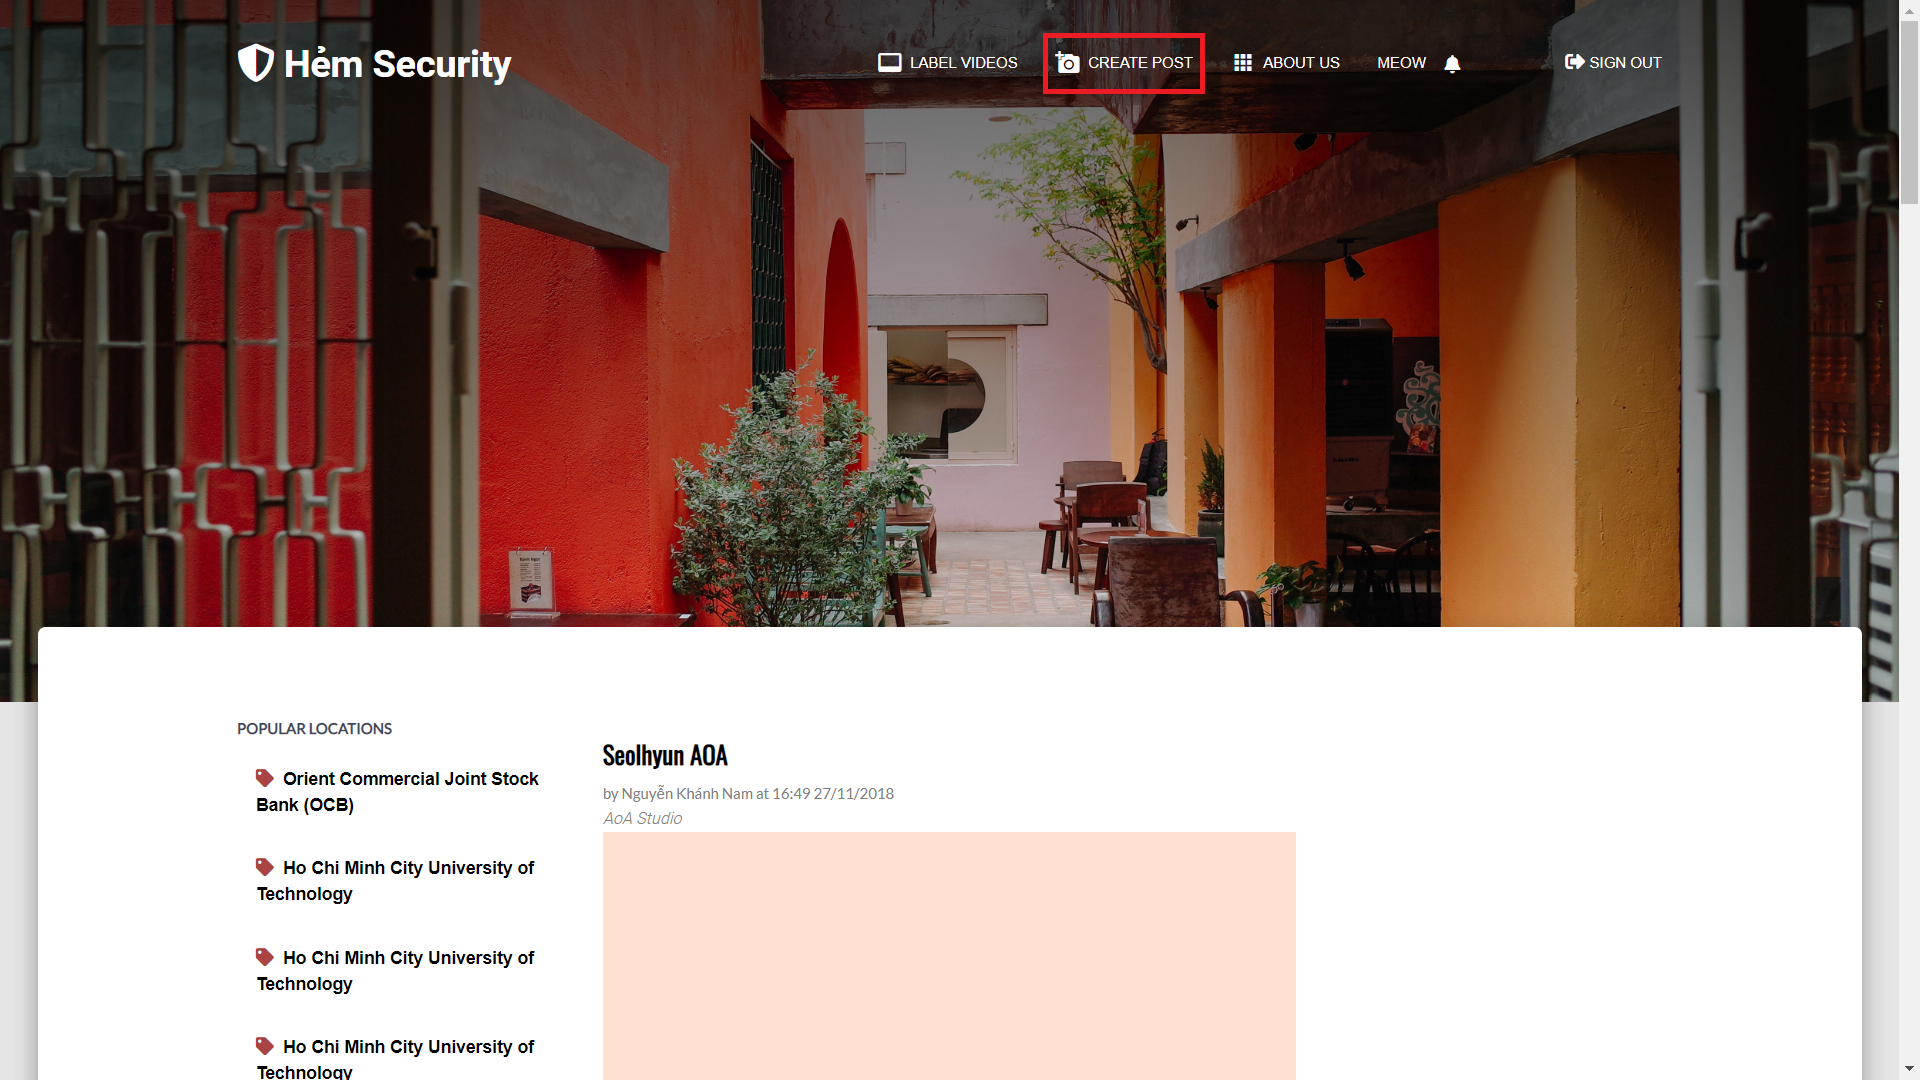
\includegraphics[width=1\columnwidth]{images/chap6/instruction7.png}
	\end{figure}
\end{center}
2. Fill in the form to and click "Create". 
\begin{center}
	\begin{figure}[H]
		\centering
		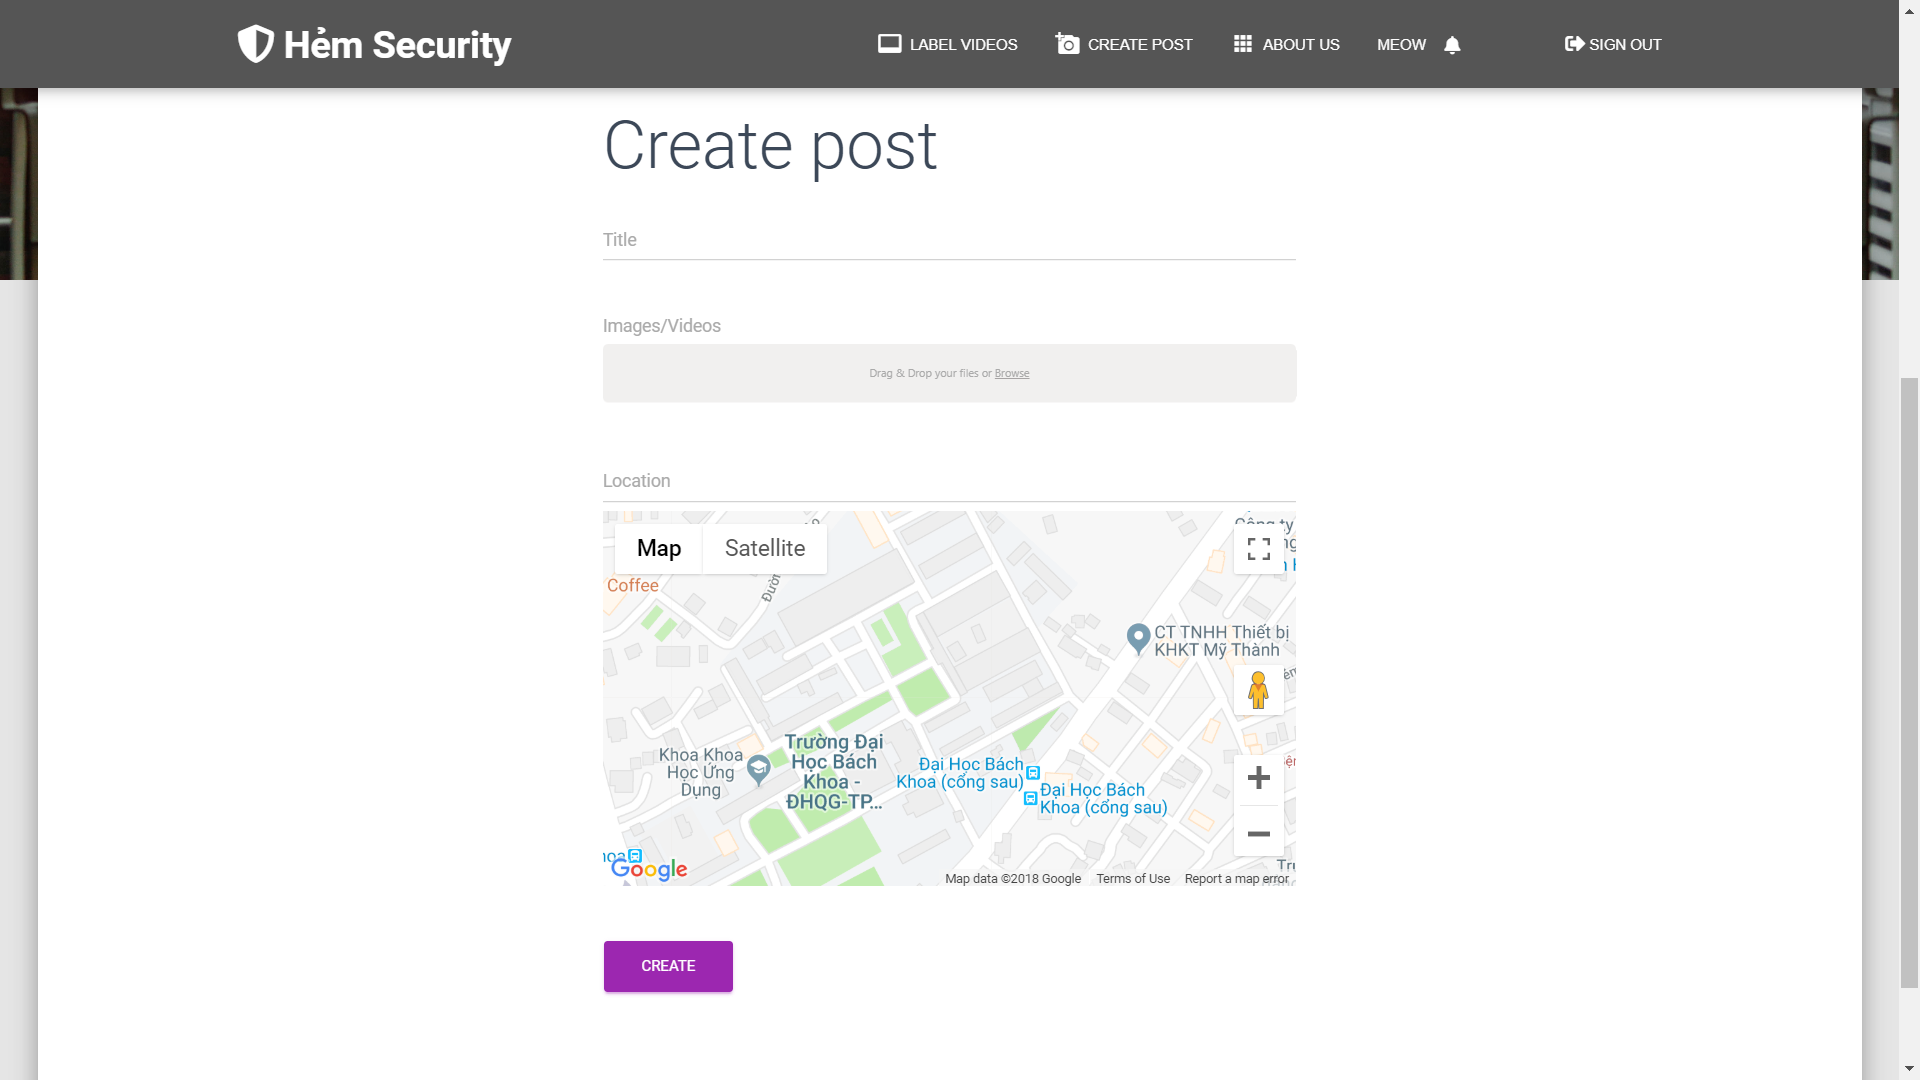
\includegraphics[width=1\columnwidth]{images/chap6/instruction8.png}
		\footcaption{Create post form}
	\end{figure}
\end{center}
\section{Subscribe a location}
1. Go to profile page and choose "All locations" tab
\begin{center}
	\begin{figure}[H]
		\centering
		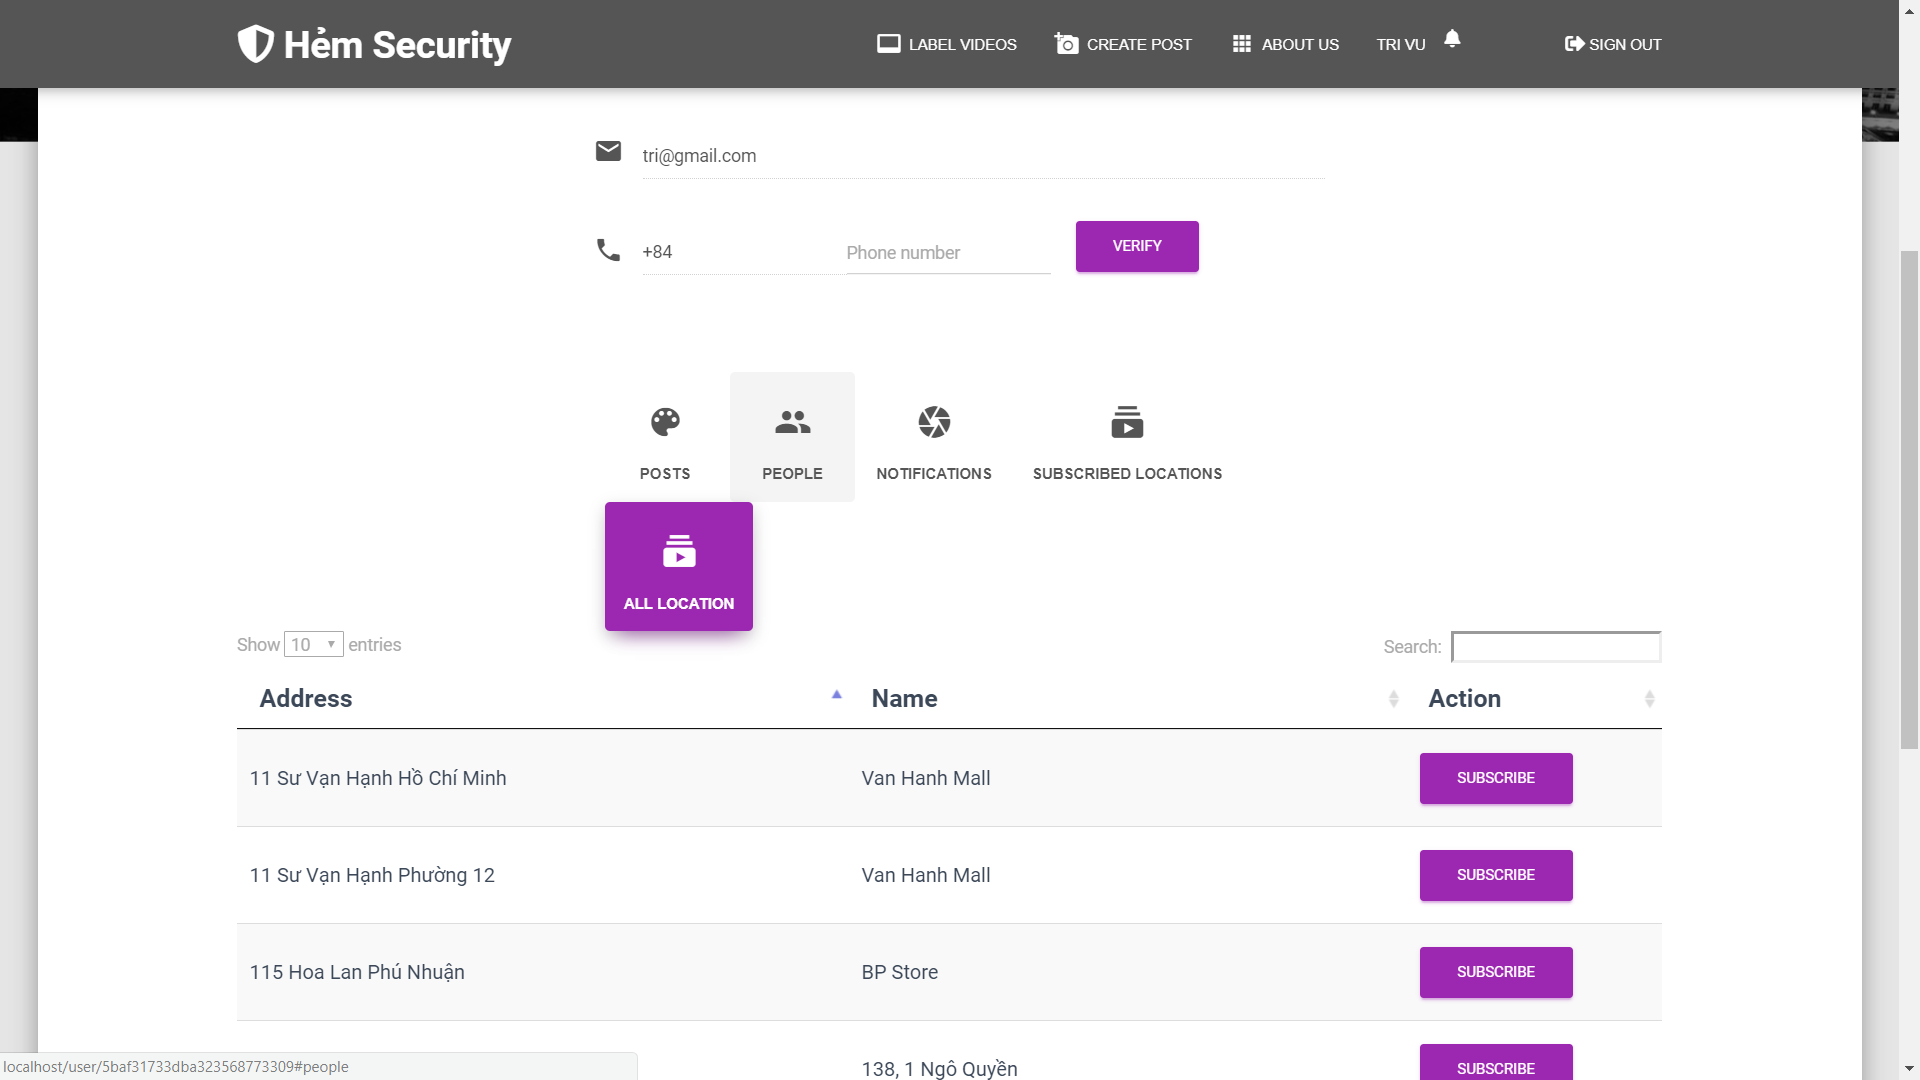
\includegraphics[width=1\columnwidth]{images/chap6/instruction9.png}
	\end{figure}
\end{center}
2. Choose a location to subscribe from the list. User will receive notification about suspicious behavior around subscribed location within a radius of 1 kilometer.   
\begin{center}
	\begin{figure}[H]
		\centering
		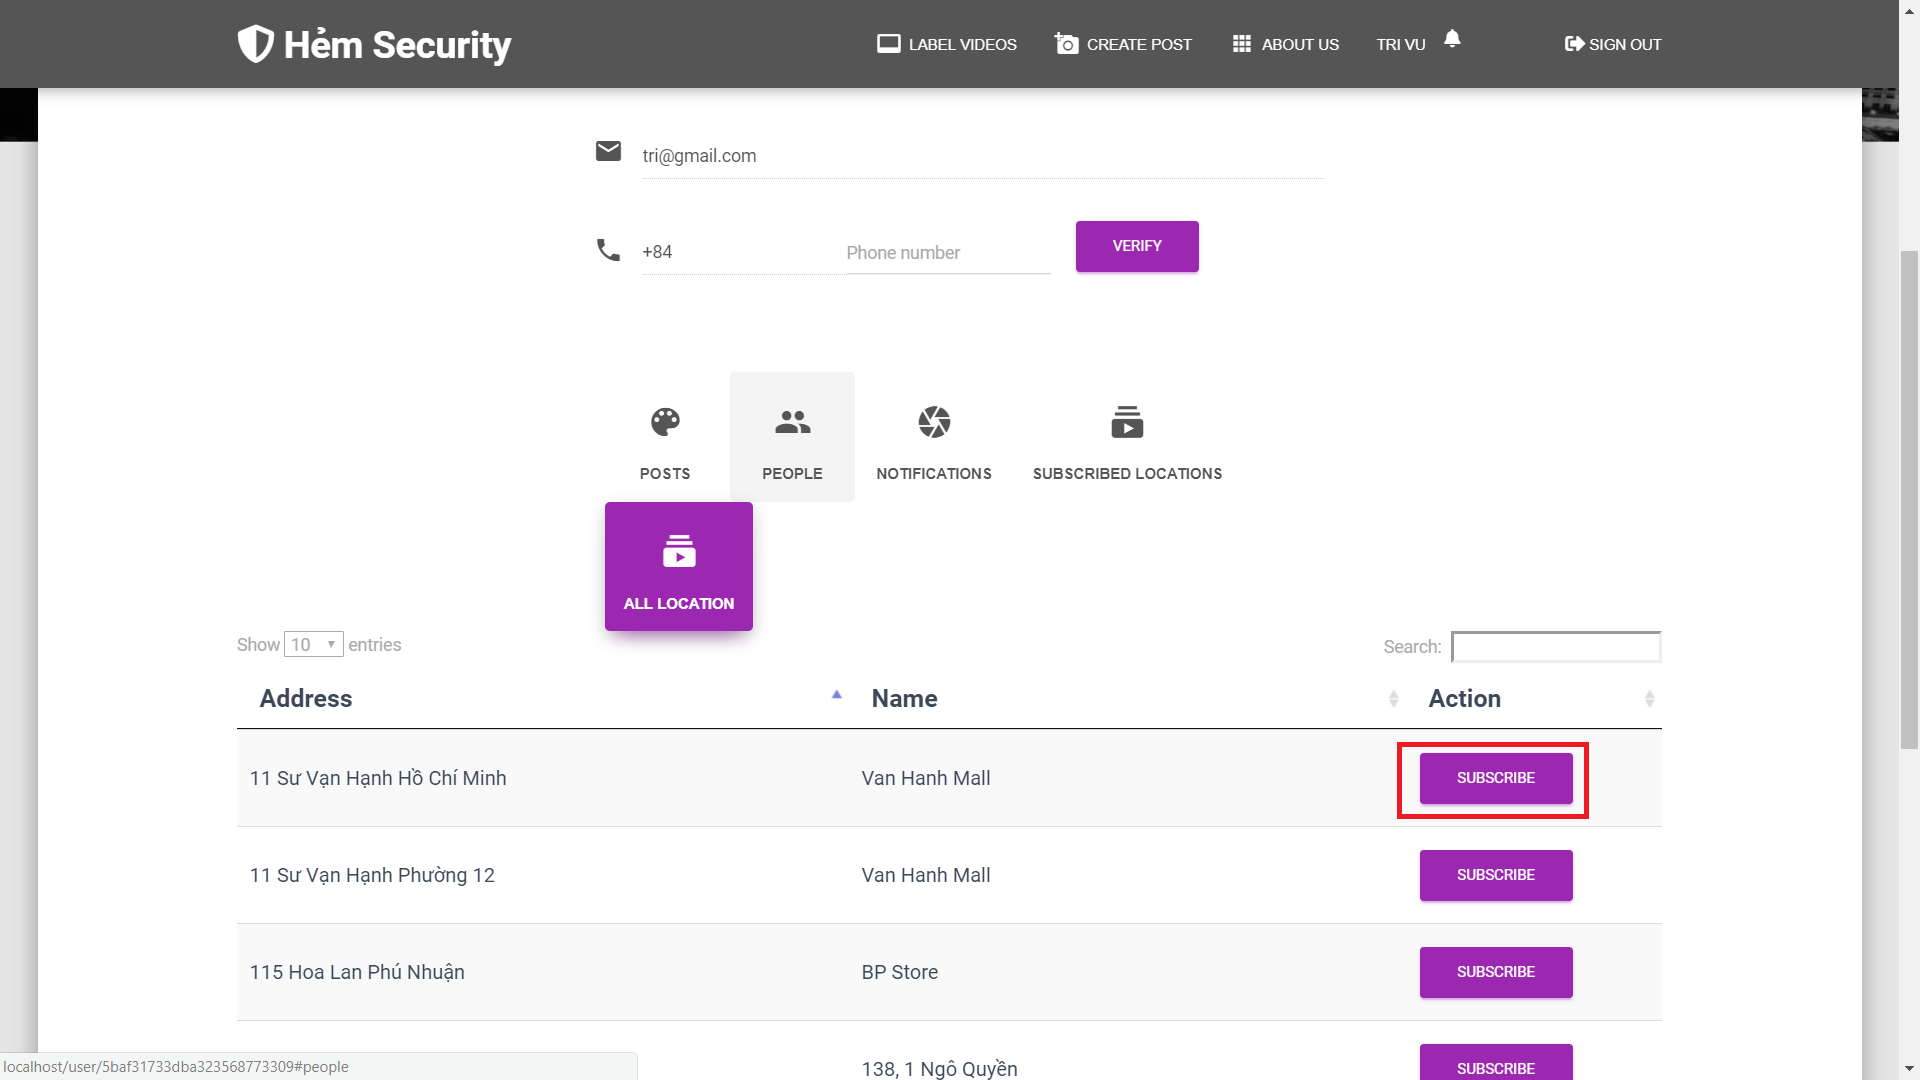
\includegraphics[width=1\columnwidth]{images/chap6/instruction10.png}
	\end{figure}
\end{center}